\documentclass[fleqn,usenatbib]{mnras}

\usepackage[T1]{fontenc}

\DeclareRobustCommand{\VAN}[3]{#2}
\let\VANthebibliography\thebibliography
\def\thebibliography{\DeclareRobustCommand{\VAN}[3]{##3}\VANthebibliography}


%%%%% AUTHORS - PLACE YOUR OWN PACKAGES HERE %%%%%

% Only include extra packages if you really need them. Common packages are:
\usepackage{graphicx}	% Including figure files
\usepackage{amsmath}	% Advanced maths commands
\usepackage{amssymb}	% Extra maths symbols
\usepackage{xcolor}
\usepackage{tikz}
\usepackage{colortbl}
\usepackage{dsfont}
\usepackage{bm}
\usetikzlibrary{arrows.meta}


%%%%%%%%%%%%%%%%%%%%%%%%%%%%%%%%%%%%%%%%%%%%%%%%%%

%%%%% AUTHORS - PLACE YOUR OWN COMMANDS HERE %%%%%
\newcommand{\jtd}[1]{ {\bf{\color{red} JTD: #1}} }
\newcommand{\unit}[1]{\bm{\hat{#1}}}

\newcommand{\parens}[1]{\left( #1 \right)}
\newcommand{\brackets}[1]{\left[ #1 \right]}
\newcommand{\quat}[1]{\widetilde{\bm{#1}}}

% Please keep new commands to a minimum, and use \newcommand not \def to avoid
% overwriting existing commands. Example:
%\newcommand{\pcm}{\,cm$^{-2}$}	% per cm-squared

%%%%%%%%%%%%%%%%%%%%%%%%%%%%%%%%%%%%%%%%%%%%%%%%%%

%%%%%%%%%%%%%%%%%%% TITLE PAGE %%%%%%%%%%%%%%%%%%%

\title[Flyby Constraints on Asteroids Interiors]{Constraining the Interiors of Asteroids Through Close Encounters}

% The list of authors, and the short list which is used in the headers.
% If you need two or more lines of authors, add an extra line using \newauthor
\author[Jack T. Dinsmore, Julien de Wit]{
Jack T. Dinsmore,$^{1}$\thanks{E-mail: jtdinsmo@mit.edu}
Julien de Wit$^{2}$
\\
% List of institutions
$^{1}$Department of Physics, Massachusetts Institute of Technology\\
$^{2}$Department of Earth, Atmospheric, and Planetary Science, Massachusetts Institute of Technology
}

% These dates will be filled out by the publisher
\date{Accepted XXX. Received YYY; in original form ZZZ}

% Enter the current year, for the copyright statements etc.
\pubyear{2022}

% Don't change these lines
\begin{document}
\label{firstpage}
\pagerange{\pageref{firstpage}--\pageref{lastpage}}
\maketitle

% Abstract of the paper
\begin{abstract}
  We investigate the degree to which asteroid interior density distributions can be extracted from rotational velocity data gathered during a close encounter. We derive the equations of motion for an rigid asteroid's orientation and angular velocity to arbitrary precision and use them to generate synthetic rotational velocity data for a representative asteroid on a close Earth flyby. Using Markov Chain Monte Carlo fits, we re-extract the density moments of the asteroid in a wide range of scenarios to measure the degree to which best fit precision is affected. Specifically, we use many injection-retrieval tests to study fit precision's dependence on the asteroid's moment of inertia, observational precision and cadence, orbital parameters, and initial spin pole direction as well as the quantity of near-pericenter data and the central body oblateness. Finally, we discuss the degeneracy between the density moments and the actual density distribution and propose four models to construct a representative density distribution from fit results.
\end{abstract}

% Select between one and six entries from the list of approved keywords.
% Don't make up new ones.
\begin{keywords}
  minor planets, asteroids: general -- methods: data analysis
\end{keywords}

%%%%%%%%%%%%%%%%%%%%%%%%%%%%%%%%%%%%%%%%%%%%%%%%%%

%%%%%%%%%%%%%%%%% BODY OF PAPER %%%%%%%%%%%%%%%%%%

\section{Introduction}

The recent increase in the quantity and quality of high-sensitivity, all-sky surveys, such as the Wide-field Infrared Survey Explorer (WISE) mission \cite{wright2010wide} has prompted the discovery of numerous asteroids, some kilometer-sized, and some predicted to encounter Earth or other planets closely in the near future. Theoretical work has demonstrated that many of these asteroids incur altered rotational velocities due to tidal torque \cite{paul88, SCHEERES2000106, ashenberg07, BOUE2009750, HouMar2017}; this two-body generalized system has been studied to several orders and with several different methods. The angular velocity changes induced by tidal torque occur both in asteroid binaries \cite{Naidu_2015}, and during planetary encounters \cite{RICHARDSON199847, scheeres2004evolution}. Such asteroids need not be tidally disrupted for their rotation state to be perturbed by tidal torque. Some examples of altered rotational velocity have recently been observed, including for (367943) Duende \cite{MOSKOVITZ2020113519, benson2020spin}, and have been predicted for the 2029 encounter of (99942) Apophis with Earth \cite{SCHEERES2005281, DEMARTINI201993}. Altered rotational states have been excluded for 1I/2017 U1 'Oumuamua \cite{KWIECINSKI2018170}. 

Such asteroid encounters have further been shown to reveal the physical properties of the encountering asteroid. Refs.~\cite{MOSKOVITZ2020113519, benson2020spin} extract best-fit dimensions for a triaxial ellipsoid model of Duende from light-curve data, and Refs.~\cite{DESCAMPS2020113726} and \cite{BERTHIER2020113990} extract bulk densities and rotational periods for asteroid binaries (3905) Doppler and (617) Patroclus respectively.

More encounter candidates are likely to be discovered in the future --- for Earth or other planets --- potentially by the James Webb Space Telescope (JWST) or Large-aperture Synoptic Survey Telescope (LSST), and general methods for assessing whether an asteroid's encounter properties are conducive to the extraction physical asteroid characteristics from light-curve data is necessary. However, such general statements are not very well studied, since much of previous research has focused on specific encounters.

Additionally, asteroid properties which are constrained only by beyond-leading-order tidal torque effects have not yet been extracted, and more research is needed to study whether these effects are, in fact, observable.

In this paper, we address these two topics by deriving a new equation of motion for an asteroid encounter system in section \ref{sec:methods}. This equation is simple and exact to arbitrary order, given assumptions reasonable for a planetary encounter (and many binary systems). It is also fast in that it allows volume integrals over the asteroid to be pre-computed. We use this equation of motion to simulate a generic asteroid flyby of Earth, and extract physical characteristics of the asteroid (specifically, density moments) from synthetic data via a Markov Chain Monte Carlo (MCMC) fit, described in section \ref{sec:fit}. We measure the uncertainties in the posterior distribution of density moments as a function of various encounter parameters such as the observational uncertainty, cadence of observation, encounter orbital parameters, and more. We express which parameters most affect the precision of fit results in section \ref{sec:results}. Finally, we propose methods to extract full density distributions with uncertainties from these density moments in section \ref{sec:distros}.

\section{Methods}
\label{sec:methods}

In this section, we describe our coordinates (section \ref{sec:coordinates}) for an encountering asteroid's position and orientation, and we parametrize its density distribution via its ``density moments'' (subsection \ref{sec:moments}). Then we derive arbitrary-order equations of motion in section \ref{sec:eom} to simulate an asteroid encounter. Finally, in section \ref{sec:sim}, we describe the simulation used to integrate the equation of motion and produce synthetic data of angular velocity over time.

\subsection{Coordinates}
\label{sec:coordinates}

Throughout this paper, we assume that the asteroid under study is on a hyperbolic flyby with pericenter $r_p$ and excess velocity $v_\infty$. We do not consider any third-body perturbations, and we assume that the body being encountered is much more massive than the asteroid (e.g., Earth, Jupiter).

We make use of two frames of reference to model this system. One is the ``inertial frame,'' with axes denoted by $\unit{X}$, $\unit{Y}$, $\unit{Z}$ and origin placed at the central body's center of mass. $\unit{X}$ points from the central body to the asteroid pericenter and $\unit{Z}$ pointing parallel to the orbit angular momentum. We will assume that the mass distribution of the central body is known in this inertial frame. In general, we use capital letters to denote vectors in the inertial frame and lowercase vectors to denote vectors in the body-fixed frame.

Our second frame is the ``body-fixed'' frame, denoted by $\unit{x}, \unit{y}, \unit{z}$. This frame is fixed with respect to the asteroid's principal axes and rotates with the asteroid, with its origin at the asteroid's center of mass. We will solve for the asteroid's mass distribution with reference to the body-fixed frame. For definiteness, we define $\unit{z}$ to be the principal axis with maximal MOI.

The relative positions of the body-fixed and inertial frames is given by the position of the asteroid. The relative orientations are of more physical interest. They are represented by $z-y-z$ Euler angles $\alpha$, $\beta$, and $\gamma$, such that a matrix $M$ rotating from the body-fixed to the inertial frame ($M\bm{r} = \bm{R}$) is given by
\begin{equation}
M = R_z(\alpha) R_y(\beta) R_z(\gamma).
\label{eqn:euler-angles}
\end{equation}
Here, $R_i(\theta)$ is a rotation around the unit vector $i$ by $\theta$ (figure \ref{fig:euler-angles}).

\begin{figure}
    \centering
    \begin{tikzpicture}
    \draw[-{Latex[length=3mm]}] (0, 0) -- (-4, 0) node[anchor=east] {$\unit x$};
    \draw[-{Latex[length=3mm]}] (0, 0) -- (2, -3) node[anchor=west] {$\unit y$};
    \draw[-{Latex[length=3mm]}] (0, 0) -- (0, 4) node[anchor=south] {$\unit z$};
    \draw[dashed, -{Latex[length=3mm]}] (0, 0) -- (3.7, -2) node[anchor=north] {$\unit n$};
    \draw[line width=0.5mm,-{Latex[length=3mm]}] (0, 0) -- (-0.5, -3) node[anchor=north] {$\unit X$};
    \draw[line width=0.5mm,-{Latex[length=3mm]}] (0, 0) -- (4, 1) node[anchor=south] {$\unit Y$};
    \draw[line width=0.5mm,-{Latex[length=3mm]}] (0, 0) -- (-1.6, 2.7) node[anchor=south] {$\unit Z$};
    \draw[->] (0.5, -0.75) arc (290:302:2.5);
    \draw (0.9, -0.9) node[anchor=center] {$\alpha$};
    \draw[->] (0, 1.2) arc (130:161:1.3);
    \draw (-0.3, 1.3) node[anchor=center] {$\beta$};
    \draw[->] (0.97, -0.52) arc (330:368:1.3);
    \draw (1.4, -0.25) node[anchor=center] {$\gamma$};
    %\draw[-{Latex[length=3mm]}] (0, 0) -- (0, 4) node[anchor=south] {$\unit Z$};
    %\draw[-{Latex[length=3mm]}] (0, 0) -- (4, 0) node[anchor=west] {$\unit Y$};
    %\draw[-{Latex[length=3mm]}] (0, 0) -- (-2, -2) node[anchor=east] {$\unit X$};
    \end{tikzpicture}
    \caption{$z-y-z$ Euler angles used in this work to express the orientation of the asteroid. Orientation is expressed as a rotation from the body-fixed axes to the inertial axes.}
    \label{fig:euler-angles}
\end{figure}


\subsection{Parameters: density moments}
\label{sec:moments}

In the next section, it will be shown that only certain aspects of the asteroid density distribution affect tidal torque. We isolate those aspects according to parameters we call ``density moments.'' First, we define the unnormalized spherical harmonics $Y_{\ell m}(\theta, \phi) = P_{\ell m}(\cos \theta)e^{im\phi}$, where $P_{\ell m}$ are the associated Legendre Polynomials without the Condon-Shortley phase. The regular and irregular spherical harmonics are also defined:
\begin{equation}
  \begin{split}
    S_{\ell m}(\bm r) &= (-1)^m (\ell - m)! \frac{Y_{\ell m}(\unit r)}{r^{\ell+1}} \\
    R_{\ell m} (\bm r) &= (-1)^m \frac{r^\ell}{(\ell + m)!} Y_{\ell m}(\unit r).
  \end{split}
\end{equation}
These spherical harmonics obey many useful identities summarized in Ref.~\cite{Gelderen1998TheSO}.

The density moments of an asteroid are defined as
\begin{equation}
  K_{\ell m} - \frac{1}{\mu_m a_m^\ell} \int_\mathcal{A} d^3 r \rho_m(\bm r) R_{\ell m}(\bm r).
  \label{eqn:klm}
\end{equation}
Note that these are complex. Here, $\mathcal{A}$ indicates the volume of the asteroid, $\mu_m$ is the mass of the asteroid, $\rho_m(\bm r)$ is the density distribution, and $a_m$ is a real length scale defined (for reasons covered later) as 
\begin{equation}
  a_m^2 = \frac{1}{\mu_m} \int_\mathcal{A} d^3 r \rho(\bm r) r^2.
  \label{eqn:am}
\end{equation}
This length scale can be thought of as akin to the radius of the asteroid (although a spherical, uniform-density asteroid has radius $\sqrt{5/3} a_m$).
Both of these equations should be computed in the body-fixed axes.

Equations \ref{eqn:klm} and \ref{eqn:am} can be extended to the central body:
\begin{equation}
  \begin{split}
    &J_{\ell m} = \frac{1}{\mu_M a_M^\ell} \int_\mathcal{B} d^3 r \rho_M(\bm r) R_{\ell m}(\bm r)\\
    &a_M^2 = \frac{1}{\mu_M} \int_\mathcal{B} d^3 r \rho(\bm r) r^2.
  \label{eqn:jlm}
  \end{split}
\end{equation}
which should be computed in the inertial axes.

Note that both $J_{\ell m}$ and $K_{\ell m}$ are unitless. We call them ``moments'' because the $R_{\ell m}(\bm r)$ contains an $r^\ell$ dependence so that $K_{\ell m}$ is the $\ell$th mass moment of the asteroid.

These moments share several key properties which we discuss before continuing. Firstly, for real mass density, properties of the spherical harmonics imply that $K_{\ell m} = (-1)^m K_{\ell, -m}^*$. Therefore, the set of $K_{\ell m}$ for $\ell < \ell_\text{max}$ provides $\ell_\text{max}^2$ degrees of freedom. However, some of these degrees of freedom are additionally constrained as discussed below.

By definition, $K_{00}=1$. Furthermore, $K_{1m} = 0$ since the body-fixed frame is centered on the asteroid center of mass. Further calculation reveals that the alignment of the body-fixed frame with the asteroid principal axes also forces $K_{21}=K_{2,-1} = 0$ and $\Im K_{22}=0$. The only physical density moments for $\ell \leq 2$ are therefore $K_{22}$ and $K_{20}$, which are related to the moment of inertia around each principal axis by
\begin{equation}
  \begin{split}
    I_x &= \frac{2}{3}\mu_m a_m^2 \parens{K_{20} - 6 K_{22} + 1}\\
    I_y &= \frac{2}{3}\mu_m a_m^2 \parens{K_{20} + 6 K_{22} + 1}\\
    I_z &= \frac{2}{3}\mu_m a_m^2 \parens{-2K_{20} + 1}.
  \end{split}
  \label{eqn:moi}
\end{equation}
Incidentally, the definition of $a_m$ was chosen to satisfy equation \ref{eqn:moi}.

The physical meaning of $K_{22}$ and $K_{20}$ can be made even more clear in the case that the asteroid is a uniform-density triaxial ellipsoid. In this case, equating equation \ref{eqn:moi} with the moments of inertia of such a body yields semi-major axes of 
\begin{equation}
  \begin{split}
  a &= \sqrt{\frac{5}{3}}a_m\sqrt{1-2K_{20}+12K_{22}}\\
  b &= \sqrt{\frac{5}{3}}a_m\sqrt{1-2K_{20}-12K_{22}}\\
  c &= \sqrt{\frac{5}{3}}a_m\sqrt{1+4K_{20}}.
  \label{eqn:ellipsoid-axes}
  \end{split}
\end{equation}

The physical meaning of the higher-order moments $K_{3m}$ can be gleaned by assessing their symmetry properties. An asteroid that is mirror-symmetric along the $\unit{x}$ axis (meaning $\rho_m(x,y,z)=\rho_m(-x,y,z)$) necessarily sets certain density moments to zero. Which density moments are zeroed by which mirror symmetries is outlined in table \ref{tab:klm-symmetries}. Note that, while no mirror symmetries set $K_{00}$, $K_{20}$, or $K_{22}=0$, mirror symmetries exist which zero all the other moments, including $K_{3m}$. $\Re K_{32}$, $K_{31}$, and $K_{30}$ are the only $K_{3m}$ components zeroed by only one axis. This will not affect our fit results for $K_{3m}$, but when we extract density distributions from $K_{3m}$, we will see that our sample shapes have most $K_{3m}=0$.

\begin{table}
  \centering
  \begin{tabular}{c|ccccccc}
    \hline
    $\ell$ & $\Re K_{\ell 3}$ & $\Im K_{\ell 3}$ & $\Re K_{\ell 2}$ & $\Im K_{\ell 2}$ & $\Re K_{\ell 1}$ & $\Im K_{\ell 1}$ & $K_{\ell 0}$ \\ \hline
    0 &  &  &  &  &  &  & -\\ 
    1 &  &  &  &  & x & y & z\\ 
    2 &  &  & - & x,y & y,z & x,z & -\\ 
    3 & x,z & y,z & z & x,y,z & x & y & z\\ \hline
  \end{tabular}
  \caption{Axes of mirror symmetry that imply zeroed density moments. For example, for mirror symmetries along $\unit y$ or $\unit z$, $\Im K_{32}=0$. Mirror symmetry along $\unit x$ means $\rho_m(x, y, z) = \rho_m(-x, y, z)$. Hyphens indicate that none of the mirror symmetries zero the moment in question. Since $r^2>0$ for $r\neq 0$, no symmetries set $a_m=0$ either.}
  \label{tab:klm-symmetries}
\end{table} 

We make one final observation about $K_{\ell m}$: the requirement that $\rho_m(\bm r) \geq 0$ everywhere restricts $K_{\ell m}$. In the case of $K_{2m}$, this fact and the constraint that $I_z$ is larger than $I_x$ or $I_y$ requires $K_{20}$ and $K_{22}$ to fall in the triangle
\begin{equation}
  -\frac{1}{4} \leq K_{20} \leq 0, \qquad |K_{22}| \leq -\frac{K_{20}}{2}.
  \label{eqn:parameter-bounds}
\end{equation}
In practice, we also observe that $|K_{3m}| < 1$; often, $|K_{3m}| < 0.01$ even. For the rest of this paper, we therefore treat $|K_{3m}| \sim 0.01$ as a practical limit on observability, although it should be understood that this is an order-of-magnitude bound.





\subsection{Tidal torque}
\label{sec:tidal-torque}

Derivations for the tidal torque experienced by a rigid body in the gravitational field of a larger mass have been computed by several previous studies \cite{paul88,HouMar2017,BOUE2009750, ashenberg07}, often in terms of the moment of inertia of the rigid body (or higher order moments of inertia), and to varying degrees of precision. 

We present a novel derivation of the tidal torque to arbitrary orders in terms of the density moments of an asteroid defined in section \ref{sec:moments}. These density moments can be pre-computed and do not have to be re-evaluated every time step. This formulation of the problem will be more useful for this study.

Throughout this paper, we assume that the asteroid remains rigid throughout the encounter. We also assume no third-body perturbations from other Solar System objects. (More precisely, we assume that all third-body perturbing objects are closer to the central body's center of mass than the asteroid perigee distance. Thus, their density moments can be included in the density moments of the central body.) For the sake of simplicity, we also assume that the density moments of the central body are known and do not evolve with time.

The gravitational potential energy of the central body is, in its most general form,
\begin{equation}
V(\bm R') = -G\int_\mathcal{B} d^3 R \rho_M(\bm R) \frac{1}{|\bm{R}-\bm{R'}|}.
\label{eqn:first-pe}
\end{equation}
where $\rho_M$ is the density distribution of the central body and $\mathcal{B}$ indicates the central body's volume. All vectors here are written in the inertial frame. Given $|\bm{R}| < |\bm{R'}|$, Ref.~\cite{Gelderen1998TheSO} gives the identity
\begin{equation}
  \frac{1}{|\bm R - \bm R'|} = \sum_{\ell, m} R_{\ell m}(\bm R) S_{\ell m}^*(\bm R'),
  \label{eqn:ylm-expansion}
\end{equation}
where the sum is shorthand for $\sum_{\ell, m} = \sum_{\ell = 0}^\infty \sum_{m=-\ell}^\ell$.
We are interested in translating the potential energy of equation \ref{eqn:first-pe} to the body-fixed frame. To do this, we let $\bm{R'} = \bm D + \bm U$, where $\bm D$ is the location of the asteroid in the inertial frame. We further define $\bm U = M\bm u$, where $\bm u$ is in the body-fixed frame and $M$ is the rotation matrix given by the Euler angles $\alpha$, $\beta$, and $\gamma$ (see section \ref{sec:coordinates}). The translation from $\bm {R'}$ to $\bm U$ is then attained by the identity 
\begin{equation}
  S_{\ell m}(\bm R') = \sum_{\ell', m'} (-1)^{\ell'}R^*_{\ell' m'}(\bm U)S_{\ell+\ell', m + m'} (\bm D),
  \label{eqn:ylm-translation}
\end{equation}  
provided by Ref.~\cite{Gelderen1998TheSO}, and from $\bm U$ to $\bm u$ is given by
\begin{equation}
  \begin{split}
    Y_{\ell m}(M\bm u) = \sum_{m'=-\ell}^\ell & (-1)^{m+m'}\sqrt{\frac{(\ell-m')!(\ell+m)!}{(\ell+m')!(\ell-m)!}} \\
    & \mathcal{D}^\ell_{mm'}(M)^* Y_{\ell m'}(\bm u).\\
  \end{split}
  \label{eqn:ylm-rotation}
\end{equation}
Here, $\mathcal{D}^\ell_{mm'}(M)$ are the Wigner-$D$ matrices, which are determined by the Euler angles $\alpha$, $\beta$, and $\gamma$ of $M$.

Equations \ref{eqn:first-pe} to \ref{eqn:ylm-rotation} then provide formula for $V(\bm u)$ expressed as a a sum of integrals over $\mathcal{B}$ of the central body density $\rho_M(\bm R)$ times $R_{\ell m}(\bm R)$. These are expressed via equation \ref{eqn:jlm} as $J_{\ell m}$.

The tidal torque experienced by the asteroid (in the body-fixed frame) is given by
\begin{equation}
  \bm{\tau}(\bm u) = \int_\mathcal{A} d^3 u \rho_m(\bm u) (\bm u \times (-\nabla_{\bm u} V(\bm u)))
\end{equation}
where $\rho_m$ is the density distribution of the asteroid and $\mathcal{A}$ indicates the volume of the asteroid. Making use of one more identity concerning the derivatives of spherical harmonics:
\begin{equation}
  \begin{split}
  \bm u \times \nabla R_{\ell m}(\bm u)=&\frac{1}{2}\Big[(i\unit x - \unit y)(\ell-m+1)R_{\ell,m-1}(\bm u)\\
  &+(i\unit x+\unit y)(\ell+m+1)R_{\ell,m+1}(\bm u)\\
  & +2im\unit z R_{\ell m}(\bm u)\Big],
  \end{split}
\end{equation}
tidal torque can now be expressed as a function only of $J_{\ell m}$, $K_{\ell m}$, and the asteroid orientation and position. Explicitly,
\begin{equation}
  \begin{split}
  \bm \tau = &G\frac{\mu_m\mu_M}{2}\left[\sum_{\ell, m} a_M^\ell J_{\ell m} \sum_{\ell', m'}a_m^{\ell'}S^*_{\ell+\ell', m + m'} (\bm D) (-1)^{\ell'}\right.\\
  &\left.\sum_{m''=-\ell'}^{\ell'} \sqrt{\frac{(\ell'-m'')!(\ell'+m'')!}{(\ell'-m')!(\ell'+m')!}}  \mathcal{D}^{\ell'}_{m'm''}(\alpha, \beta, \gamma)^* \right. \\
  &\Big((i\unit x - \unit y)(\ell'-m''+1)K_{\ell',m''-1} \\
  &+(i\unit x+\unit y)(\ell'+m''+1)K_{\ell',m''+1}+2im''\unit z K_{\ell'm''}\Big) \Bigg].
  \end{split}
  \label{eqn:tidal-torque}
\end{equation}

Equation \ref{eqn:tidal-torque} possesses a few explicit properties which we discuss before writing the asteroid equations of motion. Firstly, $K_{00}$ does not appear, so that $\bm \tau$ is independent of asteroid mass. The mean density of the asteroid is therefore not constrained by tidal torque analysis. Secondly, torque is largest when $D$ is small (as expected), with the leading order of $\bm \tau$ proportional to $D^{-3}$. Thirdly, each $J_{\ell m}K_{\ell' m'}$ term is multiplied by $(a_M/D)^\ell (a_m/D)^{\ell'}$, the latter of which especially is a small number in most cases. Equation \ref{eqn:tidal-torque} can therefore be computed approximately by removing terms of large $\ell$ and $\ell'$. For our analysis, we remove $\ell' > 3$ and we usually keep only $\ell=0$.

Further insight can be gained by remarking the value of the first order of $\bm \tau$ for particular Euler angle cases. Setting $\beta = 0$ produces diagonal Wigner-$D$ matrices, and hence $\bm \tau \parallel \unit z$ to first order. Further, the component $\tau_z$ oscillates, so that for certain values of $\alpha$ and $\gamma$, $\bm \tau = 0.$ This $\beta=0$ condition is equivalent to $\unit z \parallel \unit Z$.

For $\beta = \pi/2$, there are two interesting cases. One is for $\alpha = \phi$ or $\alpha = \pi + \phi$, where $\phi$ is the angle between the asteroid and the perigee. In this case, $\tau = 0$ to first order. The second case is $\alpha = \phi \pm \pi/2$, when again $\bm \tau \parallel \unit z$ and $\tau_z$ oscillates. At perigee ($\phi=0$), these conditions are equivalent to $\unit z \parallel \unit X$ and $\unit z \parallel \unit Y$ respectively.

The $\bm \tau \parallel \unit z$ cases are interesting because they do not induce tumbling. If velocity is $\bm \omega \parallel \unit z$ (a non-tumbling state), then $\bm \omega \parallel \bm L$ and $\bm \tau = \dot{\bm L} \parallel \dot{\bm \omega}$ so that $\bm \omega$ remains parallel to $\unit z$ and non-tumbling. These cases of torque are additionally significant because not as many terms contribute to $\tau_z$ as to $\tau_x$ and $\tau_y$, and in general we see that $|\tau_z|$ is the smallest of the torque components.

\subsection{Equations of motion}
\label{sec:eom}


The equations of motion of the asteroid position $\bm D$ are given by Newton's law of gravitation:
\begin{equation}
  \dot{\bm V} = -\frac{G \mu_M}{r^3} \bm D \qquad \dot{\bm D} = \bm V
  \label{eqn:pos-eom}
\end{equation}
Rather than derive equations of motion for the Euler angles (which suffer from gimbal lock), we instead represent the orientation of the asteroid with a quaternion $\quat q$ which can be converted into Euler angles to compute $\mathcal{D}(\alpha, \beta, \gamma)$. This quaternion evolves as 
\begin{equation}
  \dot{\quat q} = \frac{1}{2}\quat q\quat \omega.
  \label{eqn:quat-eom}
\end{equation}
for angular velocity $\bm \omega$ given in the body-fixed frame. The equations of motion of $\bm \omega$ in turn are given by
\begin{equation}
  \begin{split}
    I_x \dot \omega_1 - \omega_y \omega_z (I_y - I_z) &= \tau_x\\
    I_y \dot \omega_2 - \omega_z \omega_x (I_z - I_x) &= \tau_y\\
    I_z \dot \omega_3 - \omega_x \omega_y (I_x - I_y) &= \tau_z.
  \end{split}
  \label{eqn:omega-eom}
\end{equation}
Equations \ref{eqn:pos-eom} to \ref{eqn:omega-eom} and \ref{eqn:tidal-torque} form a set of nonlinear, first-order coupled differential equations which can be numerically integrated. They are expressed in terms of the physical parameters $\mu_{M/m}$, $a_{M/m}$, $J_{\ell m}$ and $K_{\ell m}$ given the density moment-moment of inertia relations given by equation \ref{eqn:moi}.

Note that equation \ref{eqn:omega-eom} is independent of $a_m$ to first order in $\bm \tau$, because $I_{j} \propto a_m^2$ for all $j$ and $\bm \tau \propto a_m^2$. Therefore, scaling $a_m$ merely scales the value of the sub-leading-order contributions to $\bm \tau$.


\subsection{Simulation design}
\label{sec:sim}

We built a simulation to produce angular velocity data (in the inertial frame) as a function of time. This simulation requires as input (1) the orbital parameters of the asteroid $r_p$ (perigee distance) and $v_\infty$ (hyperbolic excess velocity); (2) the cadence of angular velocity observation $\Delta t$; (3) the central body moments $J_{\ell m}$, mass $\mu_M$, and $a_m$; (4) the initial asteroid angular velocity in the inertial frame $\bm \omega_0$; (5) the asteroid radius $a_m$; and (6) the asteroid's density moments $K_{\ell m}$ and initial Euler angle $\gamma_0$. All parameters except (6) are assumed to be known to high accuracy. One can imagine that $a_m$ is determined by light-curve analysis, but if not, it is still necessary to fix $a_m$ or else the values of $K_{\ell m}$ are degenerate with $a_m$.

We further assume that the asteroid is initially not tumbling. Thus, the rotational velocity is aligned with a principal axis (assumed to be $\unit z$, which maximizes moment of inertia). This sets $\beta = 0$ and we can further choose $\alpha = 0$. Thus, only Euler angle $\gamma_0$ is necessary to provide initial data for the simulation.

We begin our simulation at $D = 10 r_p$, with velocity predicted by Kepler's laws given by the orbital parameters. Since the leading order of the equations of motion is $\ell' = 2, \ell = 0$, this corresponds roughly to a torque of $10^{-3}$ times the maximum torque at perigee. Unless otherwise indicated, the simulation is terminated at $D=10 r_p$ as well.

With the simulation inputs specified, the equations of motion were integrated via the Runge-Kutta fourth order method, with a variable time step
\begin{equation}
  dt = dt_\text{min} + 10^{-3}(dt_\text{max} - dt_\text{min}) \brackets{\parens{\frac{D}{r_p}}^3 - 1}.
\end{equation}
The parameters $dt_\text{max}$ and $dt_\text{min}$ (20 and 10 seconds respectively) were chosen such that the error was ~100 times the floating point error, and that neighboring values of $K_{\ell m}$ yielded significantly different spin pole data.





\section{Injection-retrieval tests}
\label{sec:injection-retrieval}

In this section, we discuss how the simulation presented in the previous section was used to generate synthetic data and re-extract the density moments to assess how the precision of the re-extracted moments depends on the system parameters (e.g., true density moments, orbital parameters, etc.)

\subsection{Fit process}
\label{sec:fit}
Given synthetic data, an Affine Invariant Markov Chain Monte Carlo (MCMC) Ensemble sampler was used to generate posterior distributions based on flat priors. We use the Python implementation \texttt{emcee} \cite{foreman2013emcee}. \jtd{How detailed about the MCMC do I need to be?} Our parameters were $\gamma_0$, $K_{20}$, $K_{22}$, and $K_{3m}$ (10 in total), and were bounded by $|\gamma_0| < \pi/4$, and bounds on $K_{\ell m}$ given in section \ref{sec:moments}. Note that $\gamma_0$ is degenerate with $\gamma_0 + \pi/2$ since this is equivalent to relabeling $\unit y$ as $\unit x$ and $\unit x$ as $-\unit y$. The other bounds were $|K_{3m}| < 1$.

Before the MCMC was run, local minima in the likelihood were found via the Nelder-Mead algorithm implemented in \texttt{scipy} \cite{Gao2012}. It was found that only one local minimum existed, except when $K_{22}=0$ in which case rotational symmetry caused multiple values of $\gamma_0$ to be degenerate. Walkers were initialized near this local minimum, with spread given by the inverse Hessian of the likelihood at that point. Due to the high sensitivity of the angular velocity data to density moments, the minimization procedure sometimes failed to isolate the minimum likelihood. Therefore, a simpler simulation with the $K_{3m}$ terms of equation \ref{eqn:tidal-torque} was first used to minimize likelihood as a function of $\gamma_0$ and $K_{2m}$, and then the full simulation was used to find $K_{3m}$, with $\gamma_0$ and $K_{2m}$ fixed. This tiered miniimzation process motivates us to call $\gamma_0$ and $K_{2m}$ the ``first-order parameters'' and $K_{3m}$ the ``higher order parameters.''

We further subdivided the minimization process by first minimizing with respect to data truncated at the point after perigee where $D=fr_p$ for some manually-set fraction $f$. In practice, $f=2$ often led to success. The minimum was then further refined by minimizing based on the full data, with the previous minimum as the initial guess.




\subsection{Uncertainty model}
\label{sec:uncertainty}

We model uncertainty in each spin vector $\bm \omega$ as uncorrelated with other spin vectors, and we model uncertainty in the orientation and in the period as also uncorrelated. Consider a true spin vector $\bm \omega^*$. Coordinates can be chosen in which $\bm \omega^* \parallel \unit Z$. Then, expressing the observed spin vector $\bm \omega$ in spherical coordinates, we draw the polar angle from a normal distribution with standard deviation $\sigma_\theta$ centered on zero and the azimuthal angle from a uniform distribution. We also draw the ratio $\rho=\omega/\omega^*$ from a log-normal distribution centered on one, with width $\sigma_\rho$. We generally represent $\sigma_\theta > \sigma_\rho$ under the assumption that period is better constrained by light-curve data than spin pole. Explicitly, the probability density function (PDF) of $\rho$ is 
\begin{equation}
  P(\rho) = \frac{1}{\rho\sqrt{2\pi \sigma_\rho^2}} \exp\parens{-\frac{\ln^2\rho}{2\sigma_\rho^2}}
\end{equation}
See figure \ref{fig:uncertainty-model} for a representation of the uncertainty model.

\begin{figure}
  \centering
  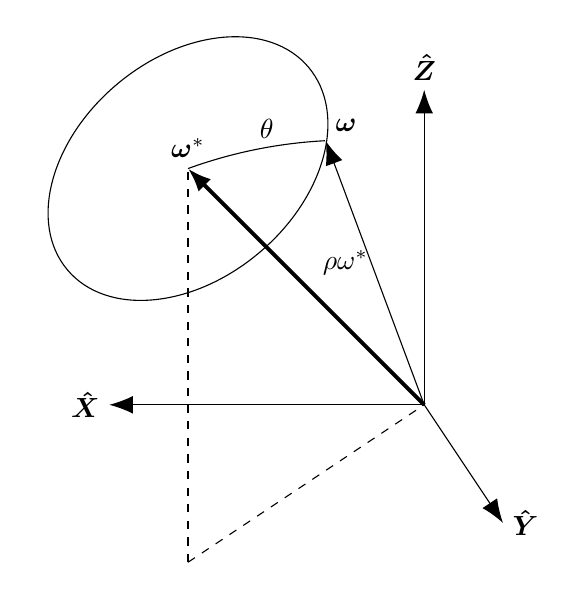
\begin{tikzpicture}
  \draw[-{Latex[length=3mm]}] (0, 0) -- (-4, 0) node[anchor=east] {$\unit X$};
  \draw[-{Latex[length=3mm]}] (0, 0) -- (1, -1.5) node[anchor=west] {$\unit Y$};
  \draw[-{Latex[length=3mm]}] (0, 0) -- (0, 4) node[anchor=south] {$\unit Z$};

  \draw[line width=0.5mm, -{Latex[length=3mm]}] (0, 0) -- (-3, 3) node[anchor=south] {$\bm \omega^*$};
  \draw[dashed] (-3, -2) -- (-3, 3);
  \draw[dashed] (-3, -2) -- (0, 0);

  \draw[-{Latex[length=3mm]}] (0, 0) -- (-1.25, 3.35) node[anchor=south west] {$\bm \omega$};
  \draw[rotate around={-50:(-3,3)}] (-3,3) ellipse (1.4 and 2);
  \draw (-3, 3) arc (110:93:6);
  \draw (-2, 3.5) node[anchor=center] {$\theta$};
  \draw (-1, 1.8) node[anchor=center] {$\rho \omega^*$};

  \end{tikzpicture}
  \caption{Diagram of the uncertainty model used to define the probability that the true spin vector $\bm \omega^*$ should be observed as $\bm \omega$. The parameter $\theta$ is drawn from a Gaussian with width $\sigma_\theta$, and $\rho$ is drawn from a log normal distribution with width $\sigma_\rho$.}
  \label{fig:uncertainty-model}
\end{figure}

The log likelihood resulting from this uncertainty model is (excluding additive constants)
\begin{equation}
  \ln \mathcal{L} = -\sum_{i = 0}\frac{\cos^{-1} (\bm \omega_i^* \cdot \bm \omega_i/(\omega_i^* \omega_i))^2}{2\sigma_\theta^2}+\frac{\ln \parens{\omega_i /\omega_i^*}^2}{2\sigma_\rho^2} + \ln\frac{\omega_i}{\omega_i^*}.
  \label{eqn:log-likelihood}
\end{equation}

In figure \ref{fig:example-data}, we present example spin data generated via this simulation. A population of one thousand asteroids with identical initial conditions except for $\gamma_0$, $K_{20}$, and $K_{22}$ were simulated on a close Earth encounter. The exact parameters used were the symmetric and asymmetric cases described in appendix \ref{app:reference-configs}. Bands containing 68.3\%, 95.5\%, and 99.7\% of the population's spin are shown, as is the spin of the reference asteroids in black.

\begin{figure*}
  \centering
  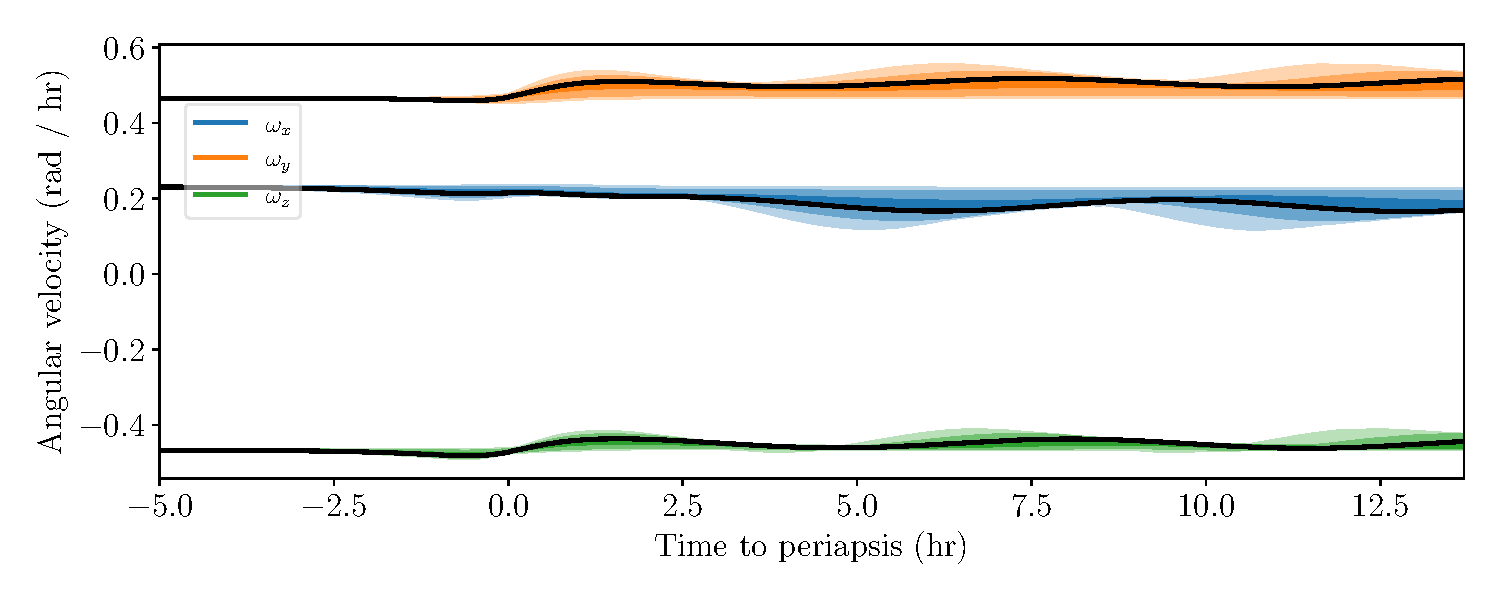
\includegraphics[width=0.7\linewidth]{figs/nominal-data-sym.pdf}
  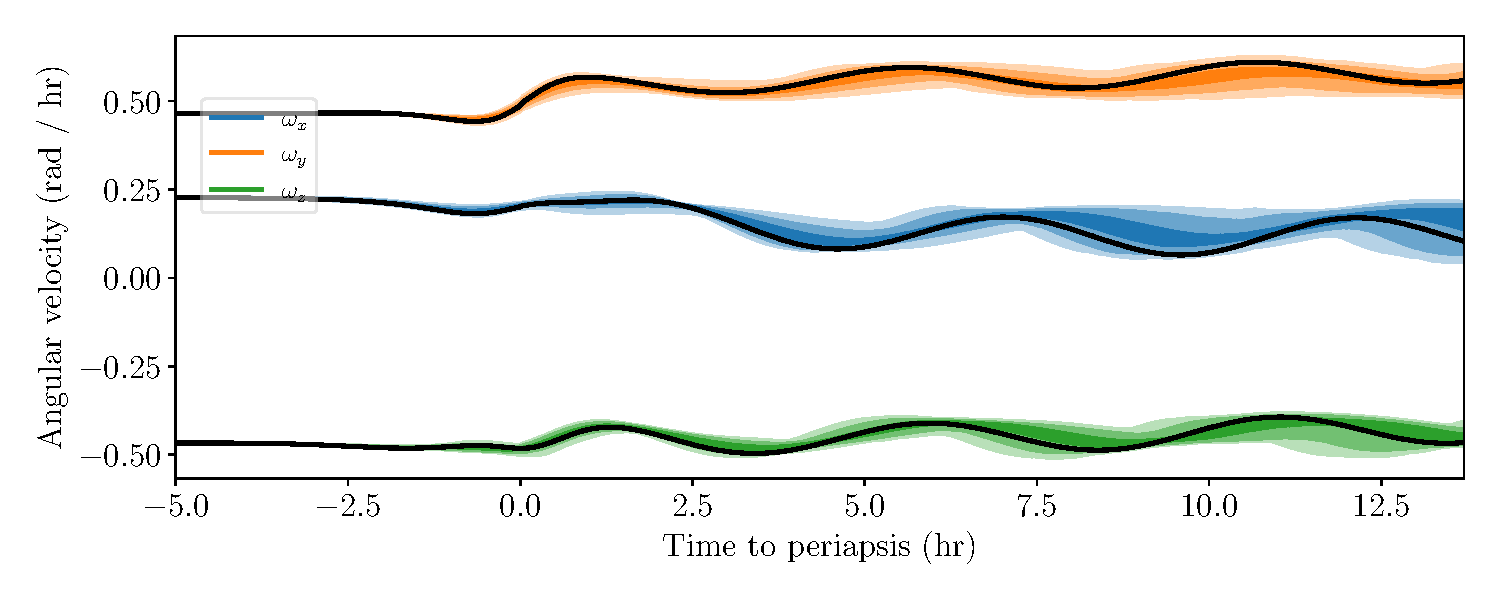
\includegraphics[width=0.7\linewidth]{figs/nominal-data-asym.pdf}
  \caption{Angular velocity data simulated for the symmetric (above) and asymmetric (below) reference asteroid densities and the reference orbit (black lines). Also plotted is the deviation of the data for posterior-PDF-distributed perturbations to the asteroid shape (bands). Bands contain 68.3\%, 95.5\%, and 99.7\% of the 1000 simulations run.}
  \label{fig:example-data}
\end{figure*}

To choose the initial values of $\gamma_0$, $K_{20}$, and $K_{22}$, spin data for the reference asteroids of appendix \ref{app:reference-configs} was first generated. Then $\gamma_0$, $K_{20}$, and $K_{22}$ were re-extracted via the fit described in section \ref{sec:fit}. The population's values for these parameters were posterior-distributed. However, the posterior distribution was widened by a factor of 1000 to make the band widths visible. Therefore, the scale of the bands in figure \ref{fig:example-data} have little meaning in an absolute sense, but they are meaningful when comparing two bands or two times in one band.

The figure illustrates the sensitivity of spin data to asteroid density moments and $\gamma_0$; Before perigee, all asteroids had similar angular velocities, but after perigee the angular velocities of the population diverged. The asymmetric case leads to more divergence than the symmetric case --- a feature which will be generalized in the next section.




\section{Results}
\label{sec:results}

In this section, we assess the sensitivity of the posterior distributions for the first-order parameters ($\gamma_0$, $K_{20}$, and $K_{22}$), and the second-order parameters ($K_{3m}$) to many possible close encounter configurations. Specifically, we test sensitivity to the encounter's orbital parameters, the degree of observational uncertainty, the asteroid's radius, the cadence of observation, the amount of data collected at perigee, the direction of the initial spin pole, the central body oblateness, and the asteroid period. These effects are presented roughly in order of how much they affect the parameter precision, from highest to lowest.

Parameter precision of 1-$\sigma$ is defined such that 68.27\% of the posterior distribution lies within 1-$\sigma$ of the mean of the posterior distribution. 2-$\sigma$ is defined likewise for 95.45\% of the posterior. The posteriors are usually roughly Gaussian, so that 1-$\sigma$ is roughly the standard deviation of the posterior.

In all cases, we use the configuration of the asymmetric reference asteroid (appendix \ref{app:reference-configs}) unless otherwise stated. We further present a test of how precision depends on cadence, asteroid period, and the duration of the flyby in appendix \ref{app:cadence-tests}, and we compare precision for a Jupiter and an Earth flyby in appendix \ref{app:jupiter-earth}.


\subsection{Orbital elements}
\label{sec:scan-orbit}
A Keplerian orbit is completely described by five parameters, but three describe the orbit's orientation with respect to the central body. The orbit can be rotated to the $\unit X \unit Y$-plane by changing the density moments of the central body. Since $J_{00}$ is unchanged by this rotation and $J_{1m}=0$, the orbit orientation is irrelevant up to the $J_{2m}$ terms of equation \ref{eqn:tidal-torque} we do not investigate them here.

We parametrize the shape of the orbit by the perigee distance $r_p$ and excess velocity $v_\infty$. Fits of the type described in section \ref{sec:fit} were run for many values of $r_p$ and $v_\infty$ and the 68 and 95\% confidence intervals are displayed in figures \ref{fig:scan-perigee} for $r_p$ and \ref{fig:scan-vex} for $v_\infty$.



\begin{figure}
  \centering
  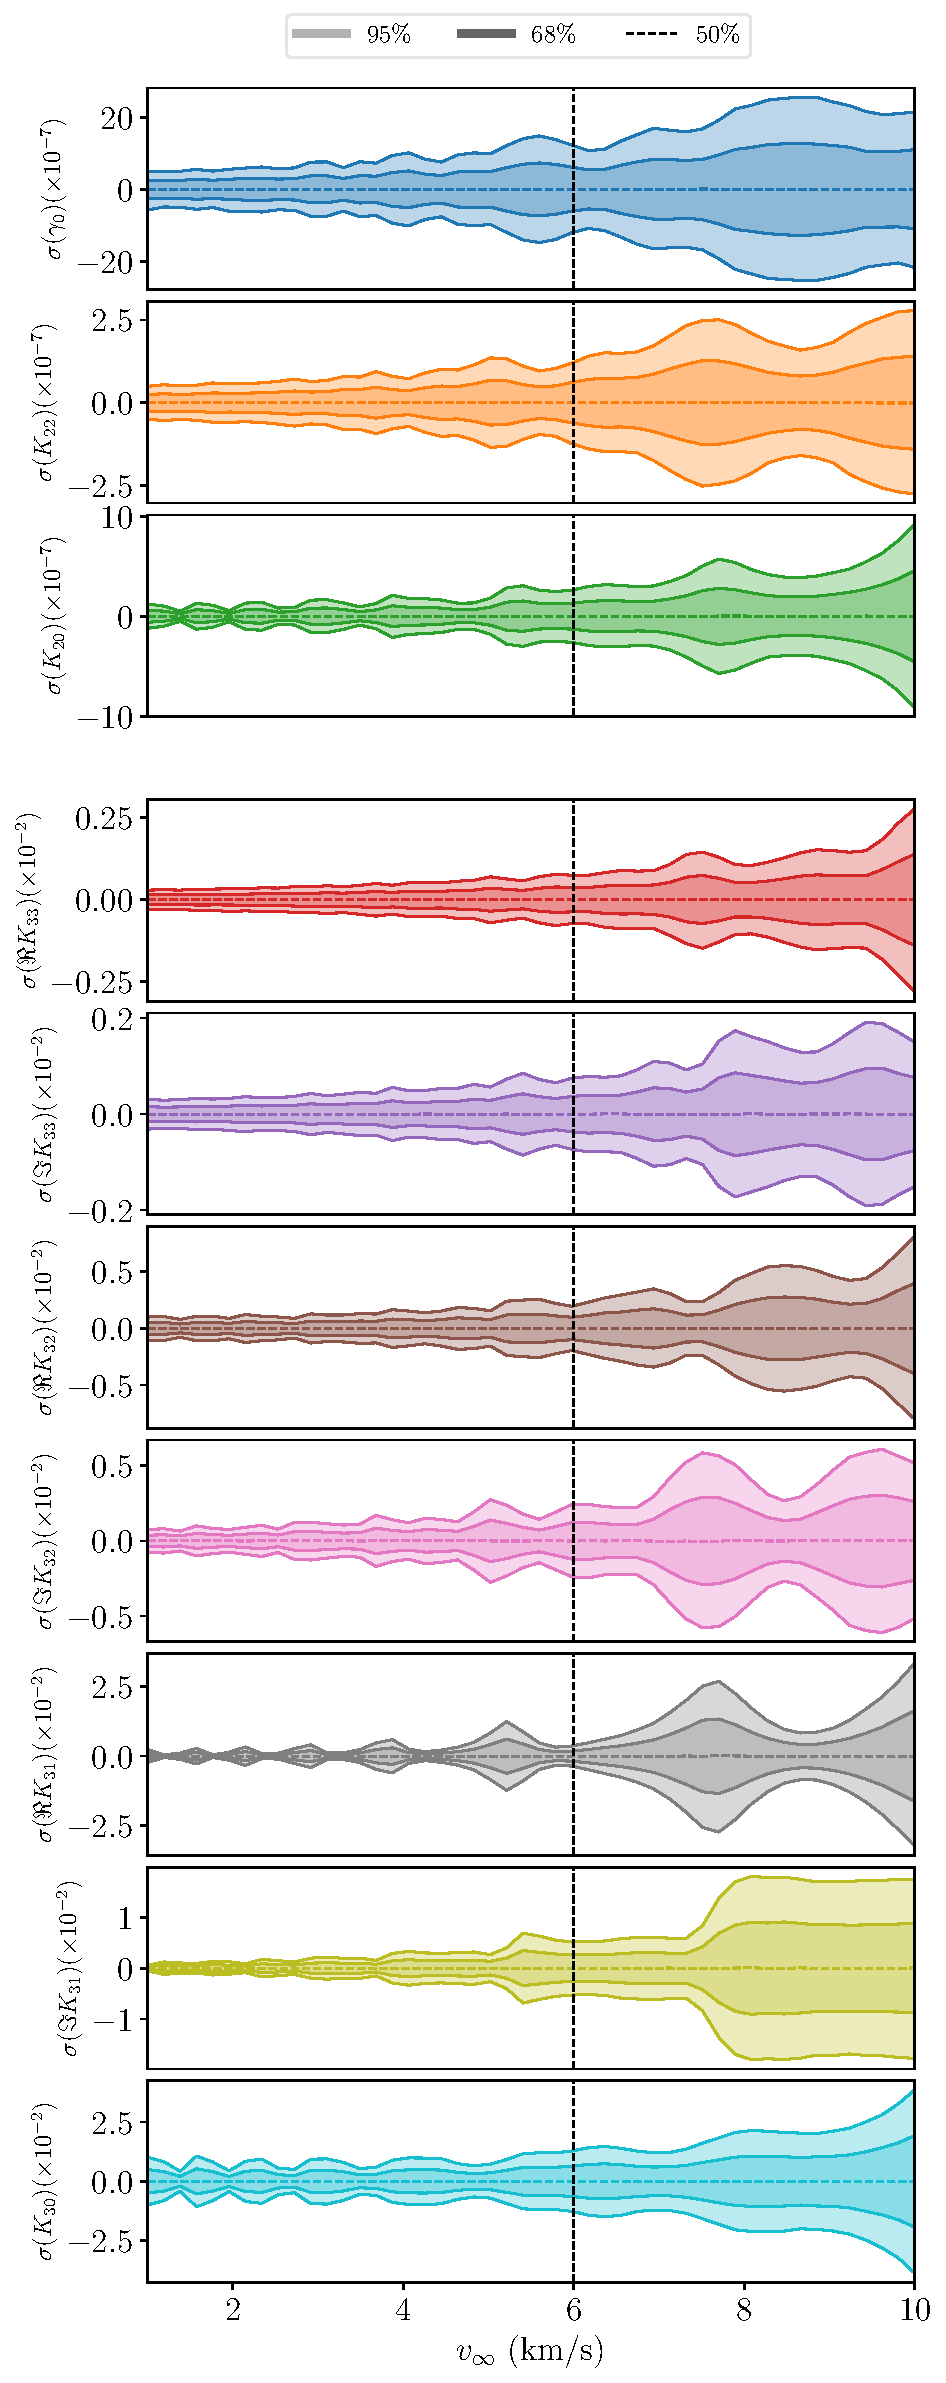
\includegraphics[height=0.89\textheight]{figs/scan-vex.pdf}
  \caption{1- and 2-$\sigma$ confidence intervals for the first-order parameter posteriors (\textit{top}) and second-order parameters (\textit{bottom}) as a function of orbital excess velocity $v_\infty$. The vertical dashed line indicates the reference asteroid value of 6 km s$^{-1}$. The red vertical lines indicate when $\sigma = 0.01$.}
  \label{fig:scan-vex}
\end{figure}

Figure \ref{fig:scan-vex} demonstrates that parameter precision does not depend strongly on excess velocity, aside from a slight trend especially in the higher order parameters for uncertainty to increase with $v_\infty$. This is likely due to the fact that larger $v_\infty$ leads to a faster and flatter orbit with less time spent close to the planet, where tidal torque is strongest. There are also smaller-scale oscillations in the uncertainty, due to the orientation of the asteroid at perigee varying. The asteroid is always simulated to start at the same orientation, but increasing $v_\infty$ decreases the time to perigee, so that the asteroid enters this region of high torque at different orientations depending on $v_\infty$. This effect explains why these small-scale oscillations have the same period for all parameters. Note that these oscillations are sometimes large enough to raise $\sigma > 0.01$.

\begin{figure}
  \centering
  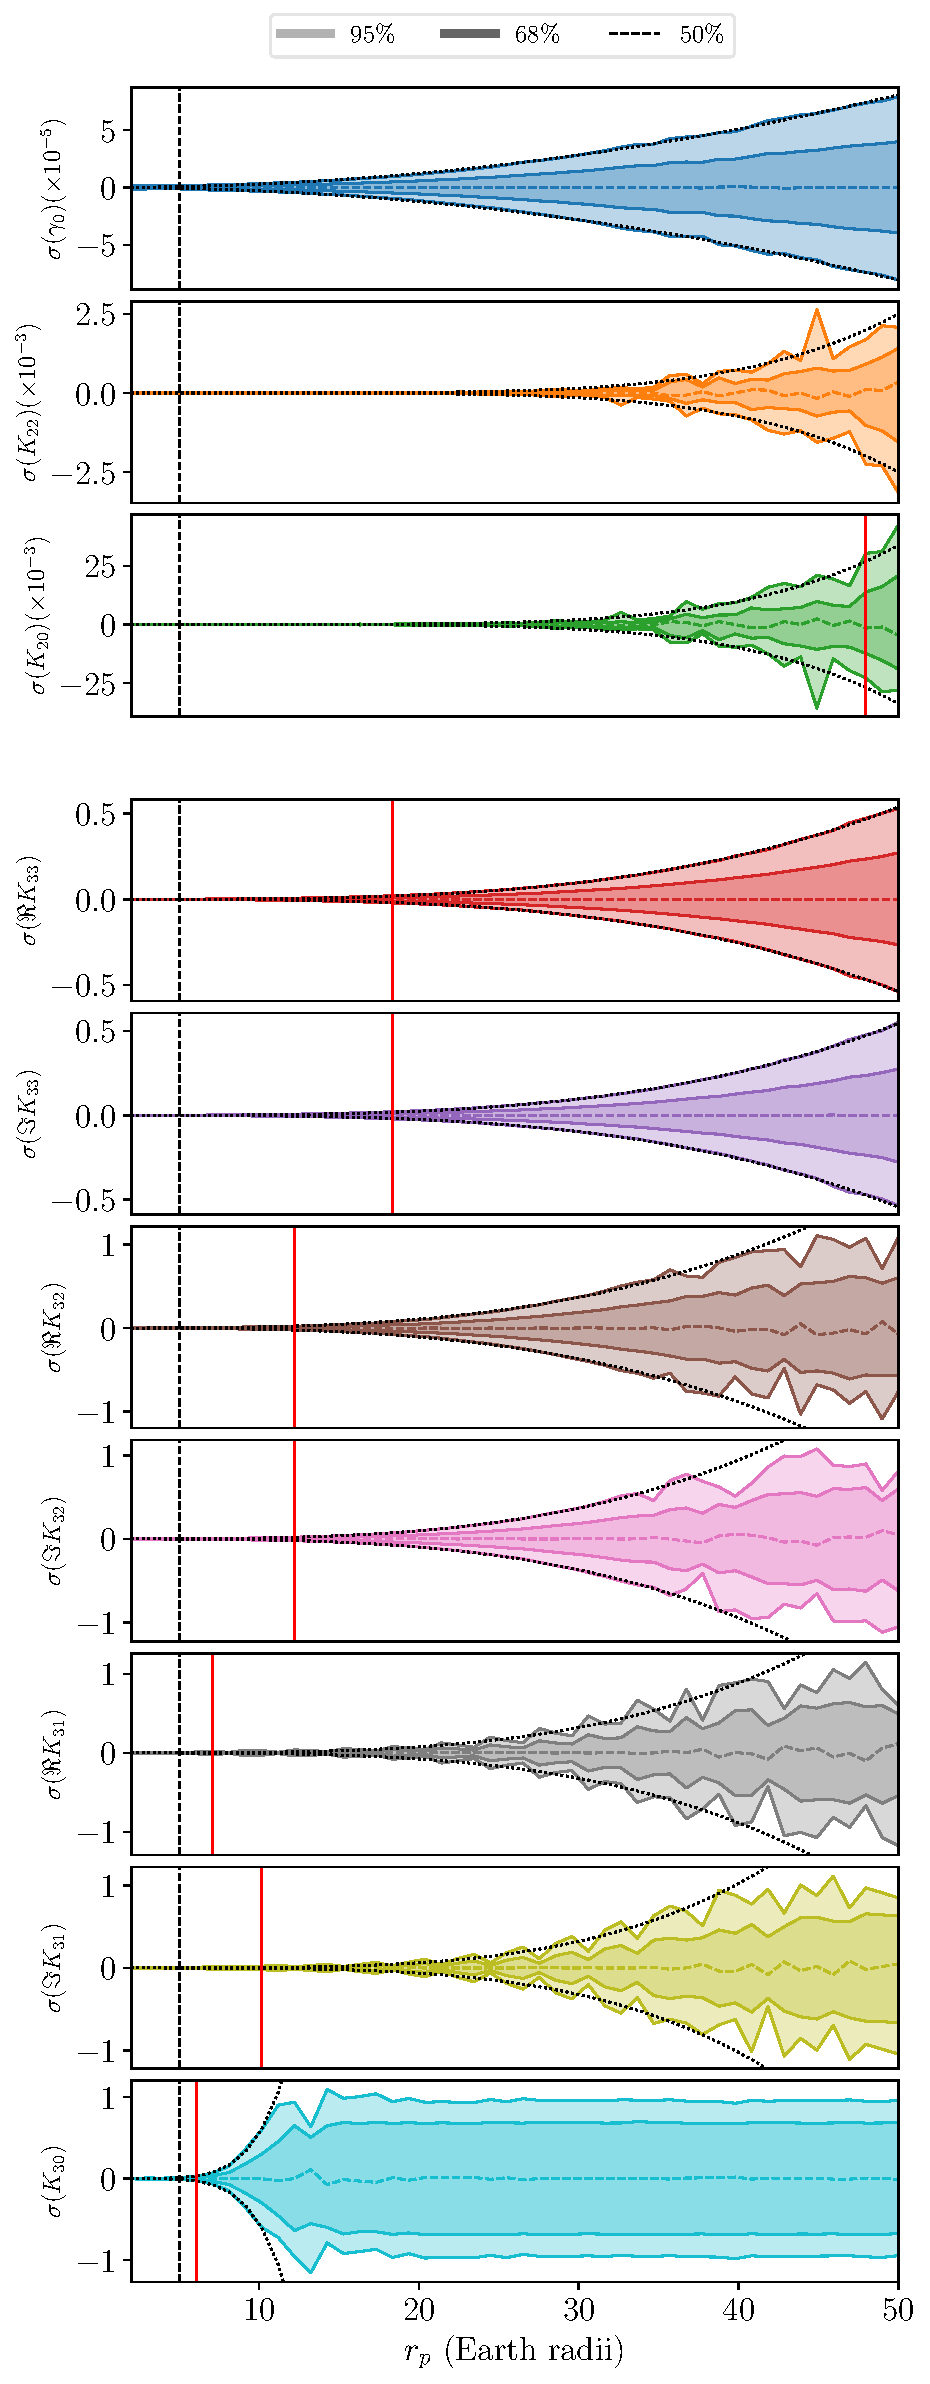
\includegraphics[height=0.89\textheight]{figs/scan-perigee.pdf}
  \caption{1- and 2-$\sigma$ confidence intervals for the first-order parameter posteriors (\textit{top}) and second-order parameters (\textit{bottom}) as a function of perigee distance $r_p$. The vertical dashed line indicates the reference asteroid value of 5 Earth radii. The dotted curve indicates a power-law fit (see text). The red vertical lines indicate when $\sigma = 0.01$.}
  \label{fig:scan-perigee}
\end{figure}

Figure \ref{fig:scan-perigee} shows much stronger dependence of parameter uncertainty on perigee distance, as expected by the factor of $(a_m/D)^{\ell'}$ present in equation \ref{eqn:tidal-torque} and mentioned in section \ref{sec:tidal-torque}. For $r_p \approx 10$ Earth radii, the most uncertain parameter $K_{30}$ fills the prior distribution, with uncertainty ranging from -1 to 1. Near $r_p \approx 40$ Earth radii, the $K_{32}$ and $K_{31}$ components also fill the prior. However, the width of the prior was arbitrarily chosen, and all the physical density distributions have $|K_{3m}|$ smaller, so the actual Earth radii cutoff at which the $K_{3m}$ parameter estimates become too imprecise to be usable likely occurs at lower $r_p$. The exact value depends on the shape of the asteroid, but for this asteroid, the figure demonstrates  $r_p \sim 10$ Earth radii causes $\sigma(K_{\ell m}) \sim 0.01$ for some moments, and 0.01 is large enough that most density distributions would then be within consistent with observations.

\begin{table}
  \centering
  \begin{tabular}{l|c}
    \hline
    Parameter & $\alpha$ \\ \hline
    $\gamma_0$ & $2.05$ \\
    $K_{22}$ & $5.47$ \\
    $K_{20}$ & $5.47$ \\ \hline
    $\Re K_{33}$ & $3.35$ \\
    $\Im K_{33}$ & $3.37$ \\
    $\Re K_{32}$ & $3.05$ \\
    $\Im K_{32}$ & $3.27$ \\
    $\Re K_{31}$ & $3.53$ \\
    $\Im K_{31}$ & $4.02$ \\
    $K_{30}$ & $5.75$ \\ \hline
  \end{tabular}
  \caption{Power law slope values for the dependence of parameter uncertainty on perigee distance $r_p$. Slope is defined by $\sigma \propto r_p^\alpha$.}
  \label{tab:scan-perigee-alpha}
\end{table}

Fitted to each of the curves in figure \ref{fig:scan-perigee} are power law uncertainties, $\sigma \propto r_p^\alpha$. These fits were performed via the method of least squares, and all data with $\sigma > 0.7$ was removed due to its sensitivity to the arbitrarily-chosen boundary of the prior. The values of $\alpha$ are shown in table \ref{tab:scan-perigee-alpha}. These slope values express how much each parameter is dependent on $r_p$. It is observed that $\gamma_0$ is least dependent on $r_p$, with $\sigma(\gamma_0) \sim r_p^2$. The other two first-order parameters are much more strongly dependent, with $\sigma \sim r_p^{5.5}$. The second-order parameters have milder slopes between 3 and 4, except for $K_{3m}$, which is fortunate from the perspective of observation, since it make render larger values of $r_p$ accessible to measuring $K_{3m}$.

The axes of figure \ref{fig:scan-perigee} show that parameters with large $m$ are more precisely determined than parameters with small $m$, as can be seen by comparing $K_{22}$ to $K_{20}$ and comparing $K_{33}$ to other $K_{3m}$ values. Large $m$ moments correspond to moments that control higher frequency fluctuations in density at the asteroid equator. This pattern of large $m$ corresponding to low uncertainty will be seen in the following sections as well.

The very strong dependence of $\sigma$ on $r_p$ makes this analysis only usable on close flybys. Fortunately, in the case of Earth, these flybys are also likely to have the best associated observational uncertainty due to their proximity. \jtd{Unfounded speculation, but hopefully this is ok.}


\subsection{Observational Uncertainty}
\label{sec:scan-uncertainty}
There are two variables, $\sigma_\theta$ and $\sigma_\rho$, which govern the observational uncertainty of the data set (defined in section \ref{sec:uncertainty}). Rather than explore the full space spanned by these two values, we measure how parameter uncertainties depend on the product of uncertainties $\sigma_\theta\sigma_\rho$ (with the radio fixed), and the ratio $\sigma_\rho / \sigma_\theta$ (with the product fixed).

We choose these metrics because we generally expect that the parameter uncertainty $\sigma$ be proportional to the observational uncertainty, but whether the dependence is stronger on $\sigma_\theta$ or $\sigma_\rho$ is not immediately clear. We get around this problem by varying $\sigma_\theta$ and $\sigma_\rho$ together and fixing their product, and measuring the posterior uncertainty $\sigma$, with $\sigma/\sigma_\theta$ shown in figure \ref{fig:scan-product}. Indeed we find that $\sigma \propto \sigma_\theta$ almost exactly, and since $\sigma_\rho / \sigma_\theta$ is fixed, we also have $\sigma \propto \sigma_\rho$. For large $\sigma_\theta \sigma_\rho$, the proportionality fails, but this is because $\sigma_\theta = 1$ at this point, so that $\sigma(K_{30}) \approx 1$ which fills the prior. Uncertainty cannot increase beyond this value.

\begin{figure}
  \centering
  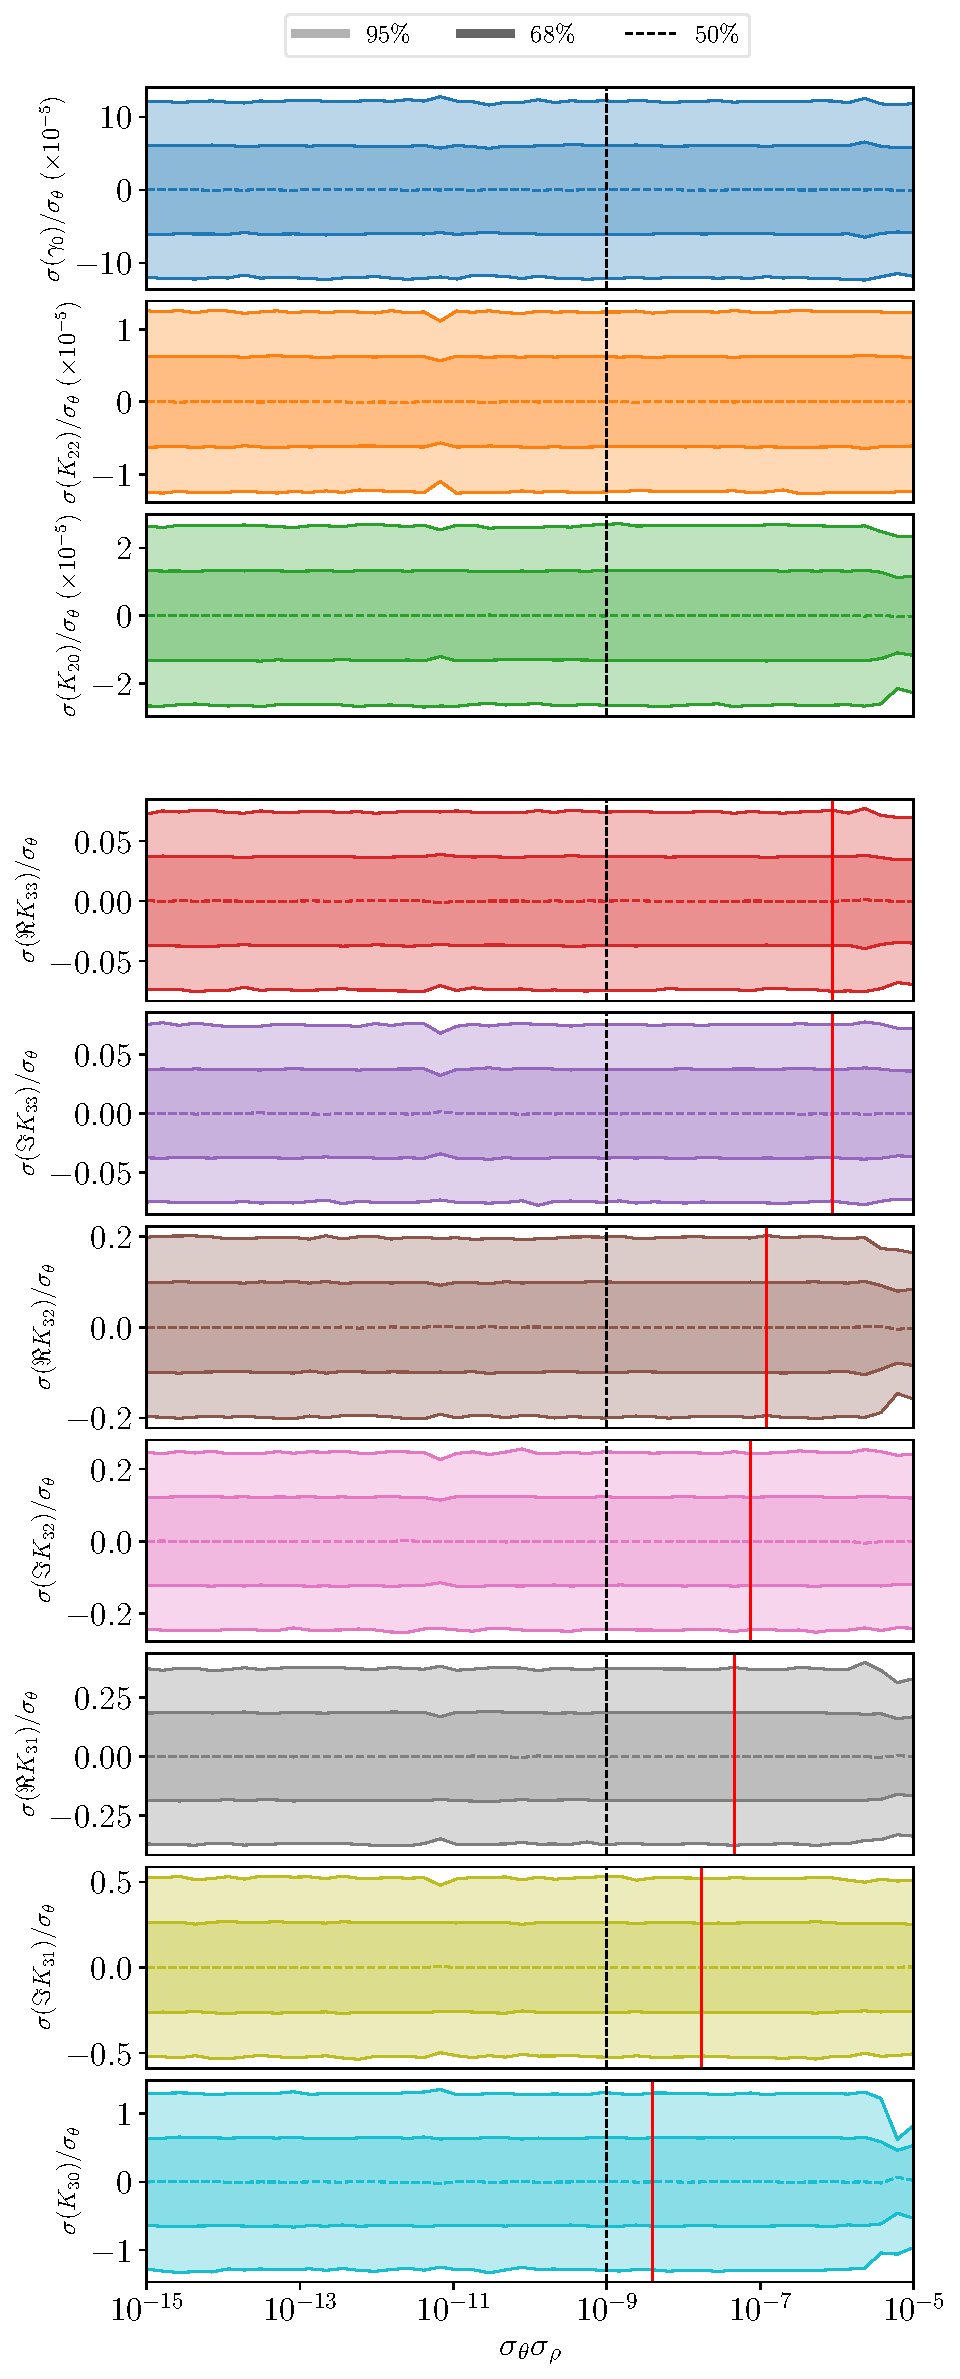
\includegraphics[height=0.89\textheight]{figs/scan-product.pdf}
  \caption{1- and 2-$\sigma$ confidence intervals divided by $\sigma_\theta$ for the first-order parameter posteriors (\textit{top}) and second-order parameters (\textit{bottom}) as a function of observational uncertainty product $\sigma_\theta \sigma_\rho$. The vertical dashed line indicates the reference asteroid value of $10^{-9}$. The red vertical lines indicate when $\sigma =0.01$.}
  \label{fig:scan-product}
\end{figure}

We also investigate the dependence of posterior uncertainty on $\sigma_\rho / \sigma_\theta$ with $\sigma_\theta \sigma_\rho$ fixed in figure \ref{fig:scan-ratio}. If we simply had $\sigma \propto \sigma_\theta \sigma_\rho$, then we would have no dependence of $\sigma$ on $\sigma_\rho / \sigma_\theta$. Any dependence shown in the figure therefore reveals some additional dependence in the model on one of the observational uncertainties.

\begin{figure}
  \centering
  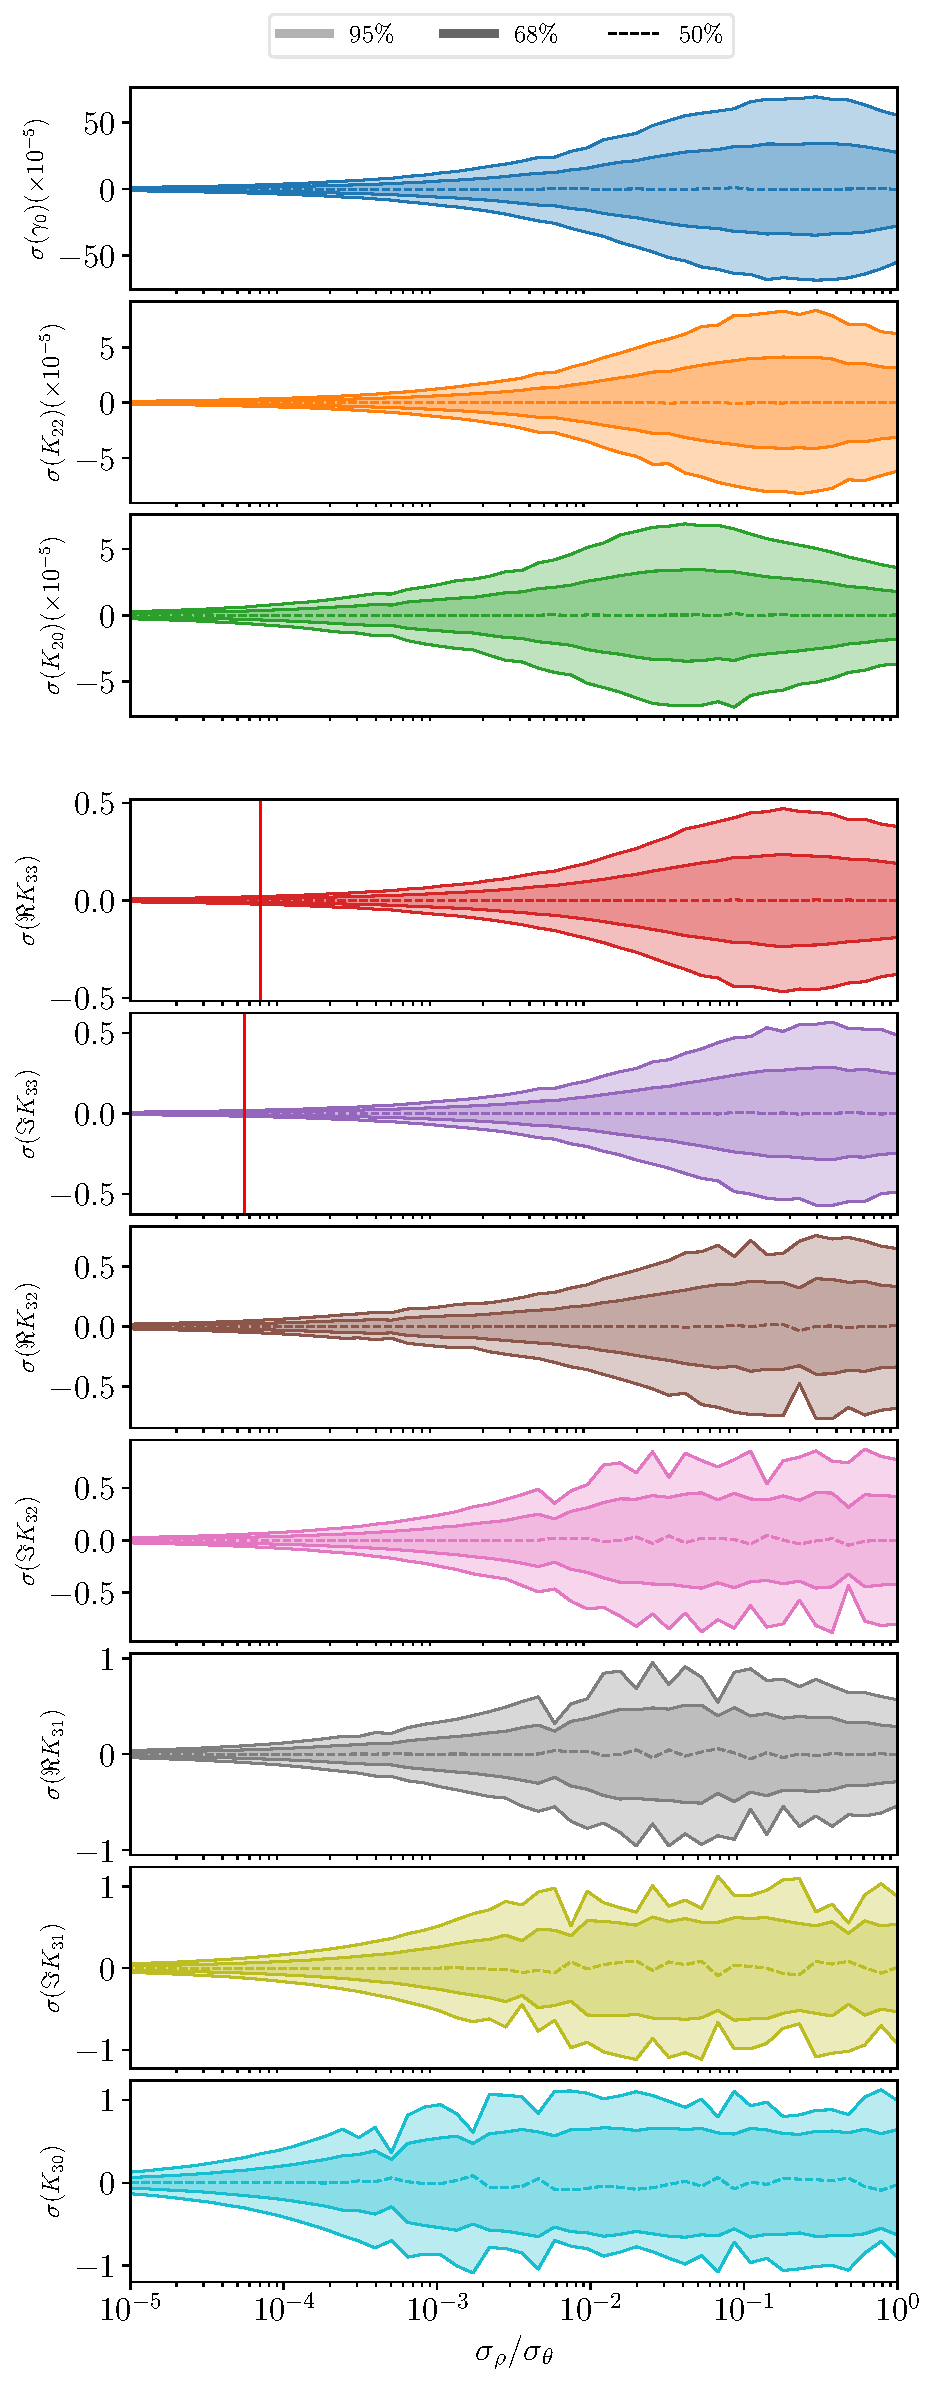
\includegraphics[height=0.89\textheight]{figs/scan-ratio.pdf}
  \caption{1- and 2-$\sigma$ confidence intervals for the first-order parameter posteriors (\textit{top}) and second-order parameters (\textit{bottom}) as a function of observational uncertainty ratios $\sigma_\rho / \sigma_\theta$. The reference asteroid value is $\sigma_\rho/ \sigma_\theta =10^{-5}$. The red vertical lines indicate when $\sigma = 0.01$. (Lines are not shown for $K_{3m}$, $m < 3$ because they coincide with the vertical axis.)}
  \label{fig:scan-ratio}
\end{figure}

Indeed, figure  \ref{fig:scan-ratio} shows increased uncertainty when $\sigma_\rho/\sigma_\theta$ is large, so that $\sigma$ depends more on $\sigma_\rho$ than on $\sigma_\theta$. We summarize this pattern my stating that, if the observer had to choose between better precision on the period or on the spin pole of the data, they should choose period. This is fortunate for observers since, \jtd{I want to say that precision on the period is better constrained by lightcurve analysis, but I have no evidence.}

Another conclusion that can be drawn from figure \ref{fig:scan-ratio} is that all parameters depend on $\sigma_\theta$ and $\sigma_\rho$ in nearly the same way (at least in the data presented). The only differences between parameters is the overall size of $\sigma$ (which shows the same dependence on $\ell$ and $m$ mentioned previously) and the fact that $\sigma$ behaves erratically when near $\pm 1$, where it fills the prior.

The location of the $\sigma > 0.01$ limit demonstrates the great incluence of observational precision on fit uncertainty: increasing $\sigma_\theta \sigma_\rho$ or $\sigma_\rho / \sigma_\theta$ by even a small amount raises $\sigma(K_{3m}) > 0.01$ in most cases.



\subsection{Asteroid shape}
\label{sec:scan-shape}

The true values of $K_{\ell m}$, $\gamma_0$, and $a_m$ affect the uncertainties in extracted density moments $\sigma$. Here, we only investigate the sensitivity of $\sigma$ on the first order parameters and $a_m$. The $K_{2m}$ moments can therefore also be viewed as the axes of a uniform density triaxial ellipsoid (equation \ref{eqn:ellipsoid-axes}).

In figure \ref{fig:scan-space-sigma}, we show the 1-$\sigma$ confidence intervals as a function of $K_{20}$ and $K_{22}$, or alternatively $a/c$ and $b/c$. We use axis ratios rather than the values of $a$, $b$, and $c$ exactly to remove the $a_m$ dependence of equation \ref{eqn:ellipsoid-axes}. The figure shows large uncertainty in $\gamma_0$ for $K_{22}=0$, or $a/c=b/c$, because $K_{20}$ is rotationally symmetric around $\unit z$, and $\gamma_0$ is the initial orientation with respect to the $\unit z$ axis. The two are uncorrelated and therefore the data has no physical dependence on $\gamma_0$ when $K_{22}=0$. This induces degeneracy in the model which inflates uncertainties, not only in $\gamma_0$ but also the other components.

\begin{figure*}
  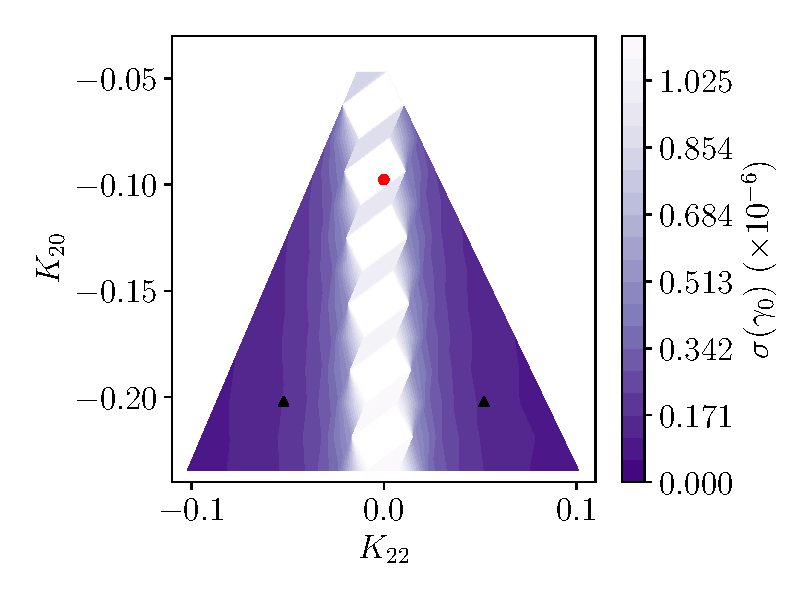
\includegraphics[width=0.33\textwidth]{figs/probe-space-theta-1-sigma.pdf}\hfill
  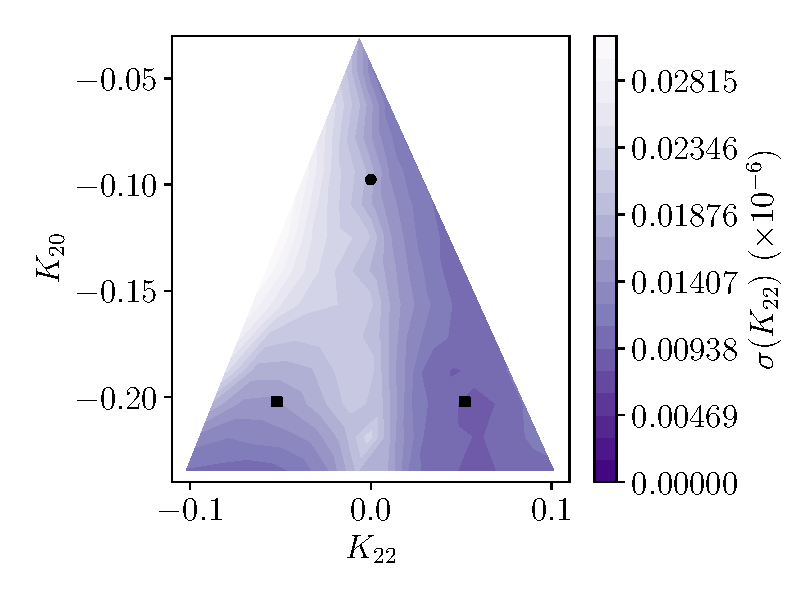
\includegraphics[width=0.33\textwidth]{figs/probe-space-theta-2-sigma.pdf}\hfill
  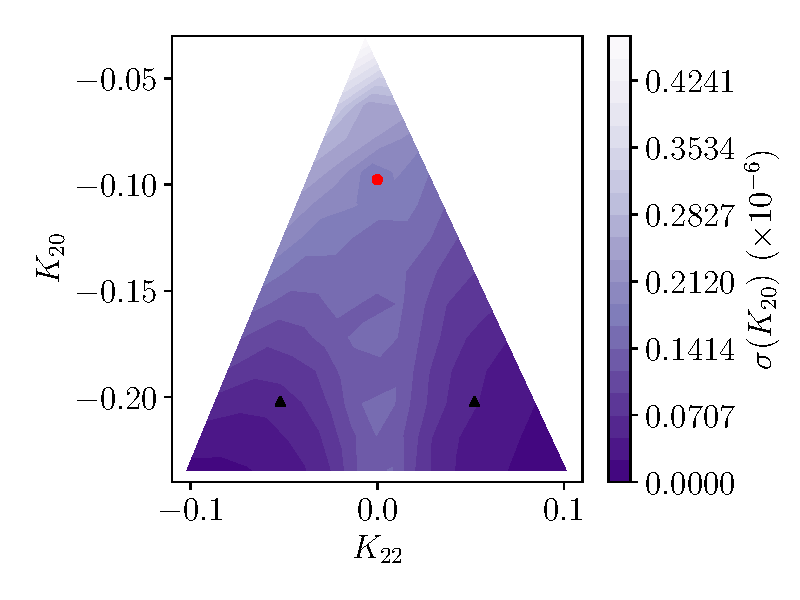
\includegraphics[width=0.33\textwidth]{figs/probe-space-theta-3-sigma.pdf}

  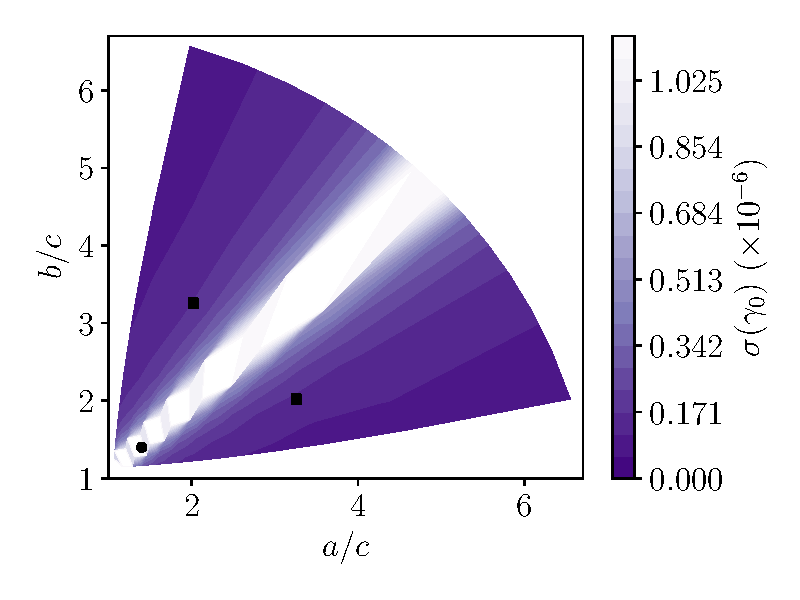
\includegraphics[width=0.33\textwidth]{figs/probe-space-ab-1-sigma.pdf}\hfill
  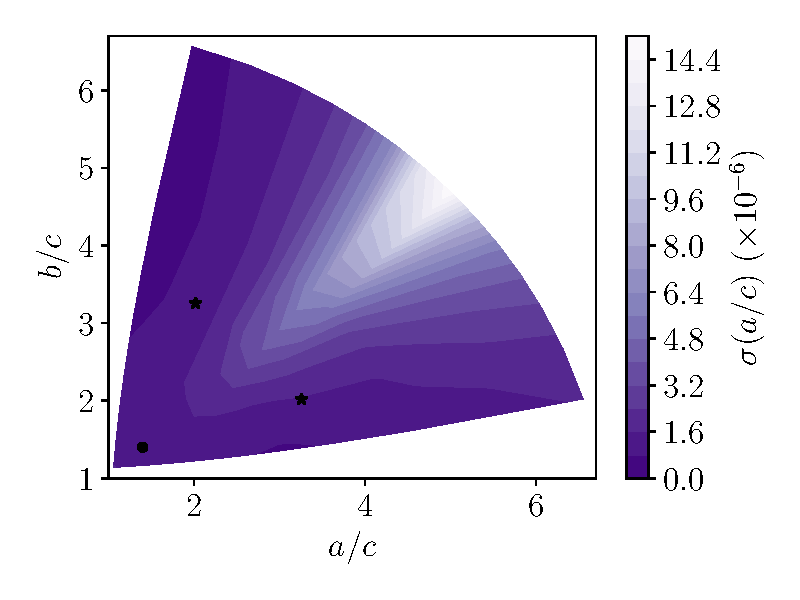
\includegraphics[width=0.33\textwidth]{figs/probe-space-ab-a-sigma.pdf}\hfill
  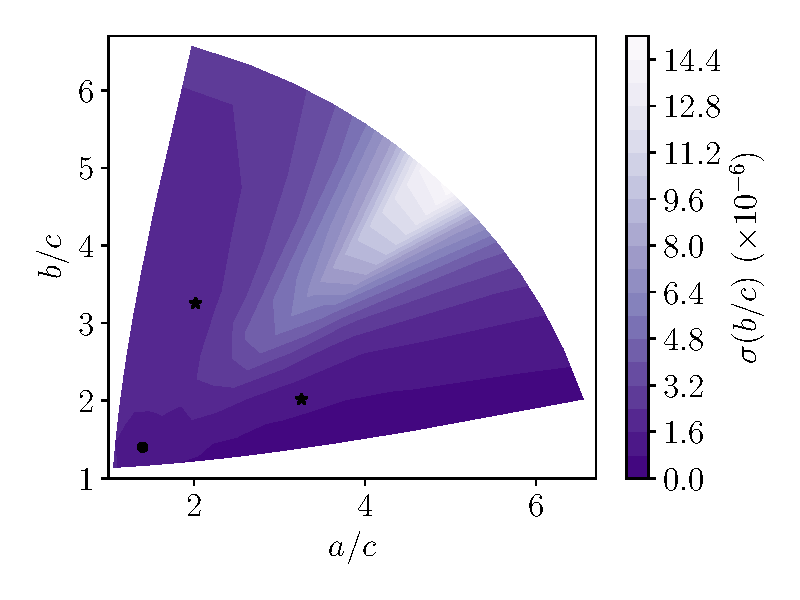
\includegraphics[width=0.33\textwidth]{figs/probe-space-ab-b-sigma.pdf}

  \caption{1-$\sigma$ confidence interval for fit parameters $\gamma_0$, $K_{22}$, and $K_{20}$ (\textit{top row}) and $\gamma_0$, $a/c$, and $b/c$ (\textit{bottom row}). Also shown as black points are the reference asteroid shapes; the symmetric case is marked with a circle and the asymmetric with a square.}
  \label{fig:scan-space-sigma}
\end{figure*}

To remove the inflated uncertainty, one could assume a rotationally symmetric asteroid with free parameters $K_{20}$ and $K_{30}$ only and run a fit. For a nearly rotationally symmetric asteroid however, a new parametrization is necessary which does not contain the ill-constrained $\gamma_0$ parameter. This task is beyond the scope of this paper, so we consider mostly asymmetric asteroids throughout.

Figure \ref{fig:scan-space-sigma} also shows low uncertainty for highly asymmetric asteroids, where $b/c$ and $a/c$ are very different or when $|K_{22}|$ is large. Additionally, $\sigma(K_{20})$ and $\sigma(K_{22})$ increase for large $K_{20}$, which is large axis ratios in the ellipsoid case (non-sphericity). For flat, disk-like asteroids, a different parametrization might therefore be more appropriate.

Figure \ref{fig:scan-space-corr} displays the correlation between the first-order parameters for reference. They show that $\gamma_0$ and $K_{22}$ are highly correlated for asymmetric asteroids, while $\gamma_0$ and $K_{20}$ are generally uncorrelated. This is expected $K_{22}$ is dependent on the orientation of the asteroid and $K_{20}$ is not. They also show that $K_{22}$ and $K_{20}$ are usually correlated, and that $a/c$ and $b/c$ are highly correlated. The latter is expected due to the $1/c$ dependence. As for the former, this correlation could likely be removed by an alternate parametrization, reducing uncertainties in the shape parameters. However, it is not clear whether these new parameters would have an obvious physical interpretation or whether they would be useful.

\begin{figure*}
  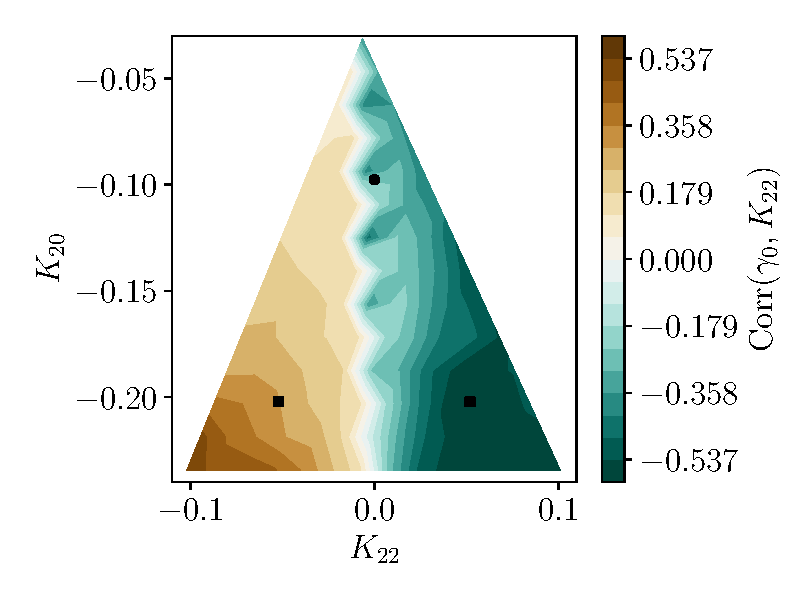
\includegraphics[width=0.33\textwidth]{figs/probe-space-corr12.pdf}\hfill
  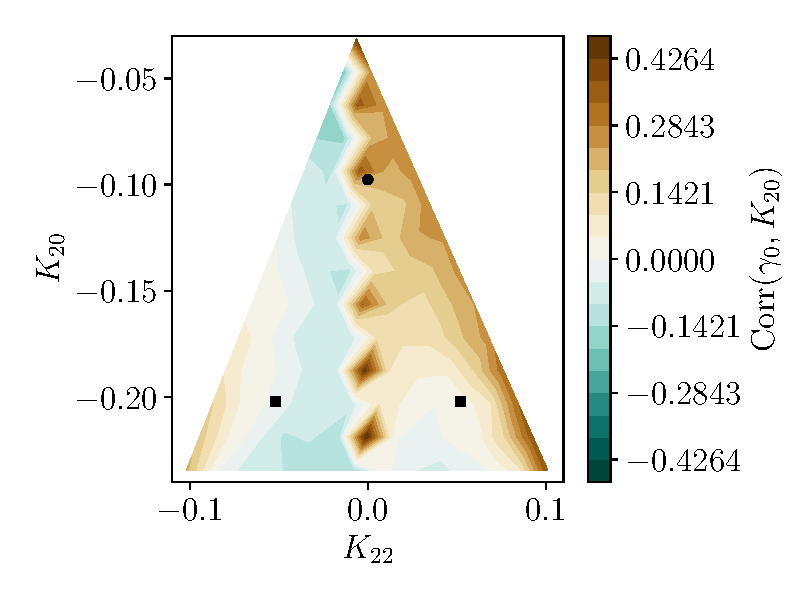
\includegraphics[width=0.33\textwidth]{figs/probe-space-corr13.pdf}\hfill
  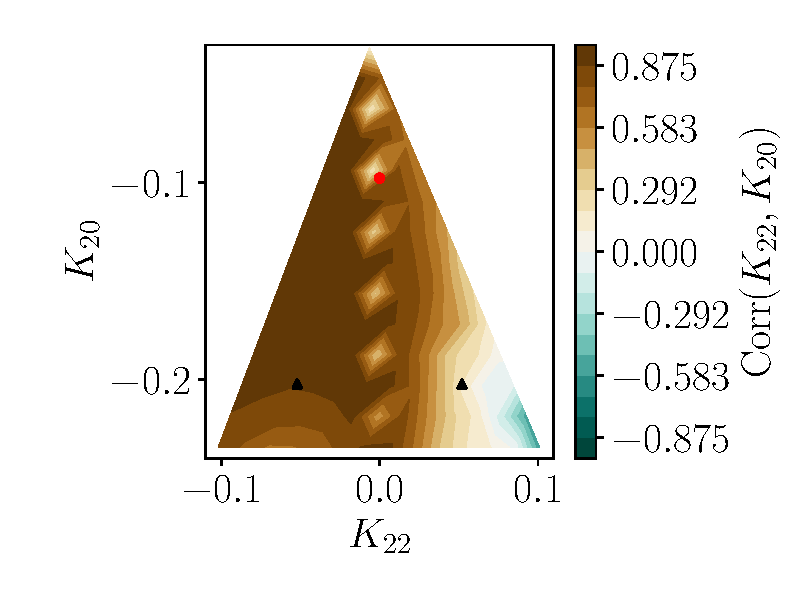
\includegraphics[width=0.33\textwidth]{figs/probe-space-corr23.pdf}

  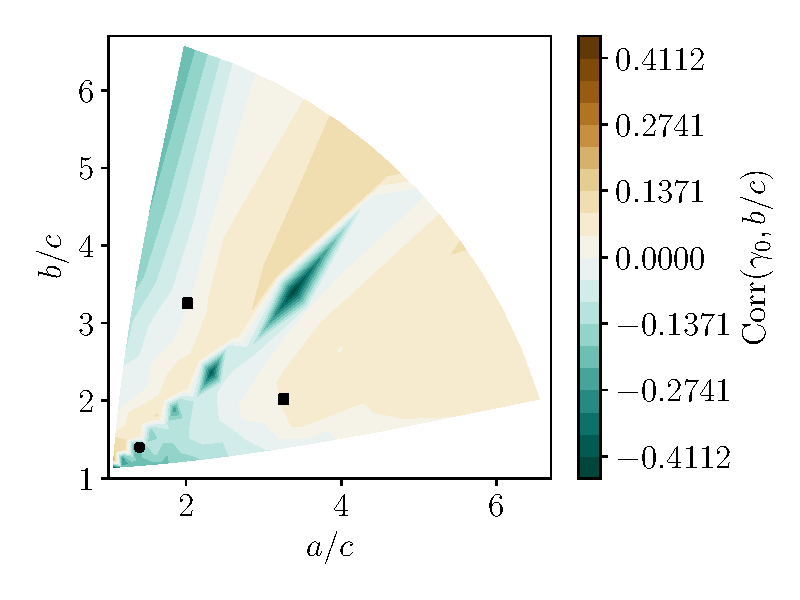
\includegraphics[width=0.33\textwidth]{figs/probe-space-ab-1b.pdf}\hfill
  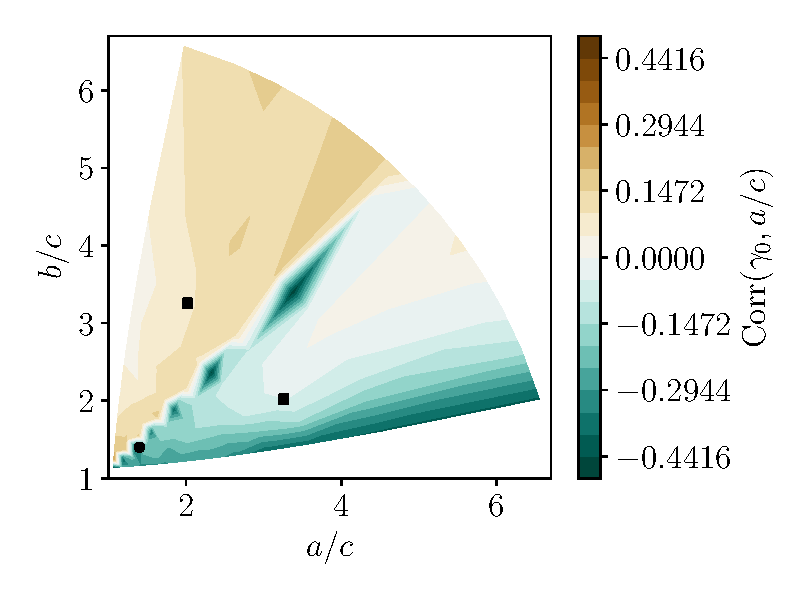
\includegraphics[width=0.33\textwidth]{figs/probe-space-ab-1a.pdf}\hfill
  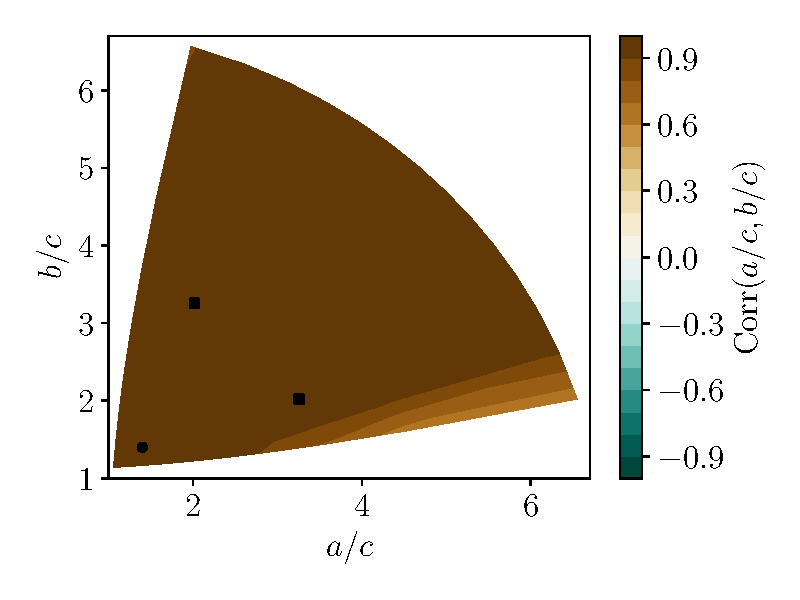
\includegraphics[width=0.33\textwidth]{figs/probe-space-ab-ab.pdf}
  
  \caption{Correlations between parameter posteriors for fit parameters $\gamma_0$, $K_{22}$, and $K_{20}$ (\textit{top row}) and $\gamma_0$, $a/c$, and $b/c$ (\textit{bottom row}).  Also shown as black points are the reference asteroid shapes; the symmetric case is marked with a circle and the asymmetric with a square.}
  \label{fig:scan-space-corr}
\end{figure*}

Overall, the variation in the uncertainties on $K_{20}$ and $K_{22}$ (the first order density moments) is present but largely smooth across their allowed parameter space, as is their correlation (except the large $K_{22}$ corner). It therefore seems reasonable to use the asymmetric asteroid shape as a stand-in for an unknown's asteroid shape when simulating a flyby, as we do in this paper. The uncertainty then can be expected to differ across other shapes by a factor of about two or less.



\subsection{Cadence}
\label{sec:scan-cadence}

The time between observations of asteroid angular velocity, or cadence, may vary depending on the observational schedule of the observing telescopes. We measure how the posterior uncertainty $\sigma$ varies with cadence ranging from two minutes to one hour in figure \ref{fig:scan-cadence}.

\begin{figure}
  \centering
  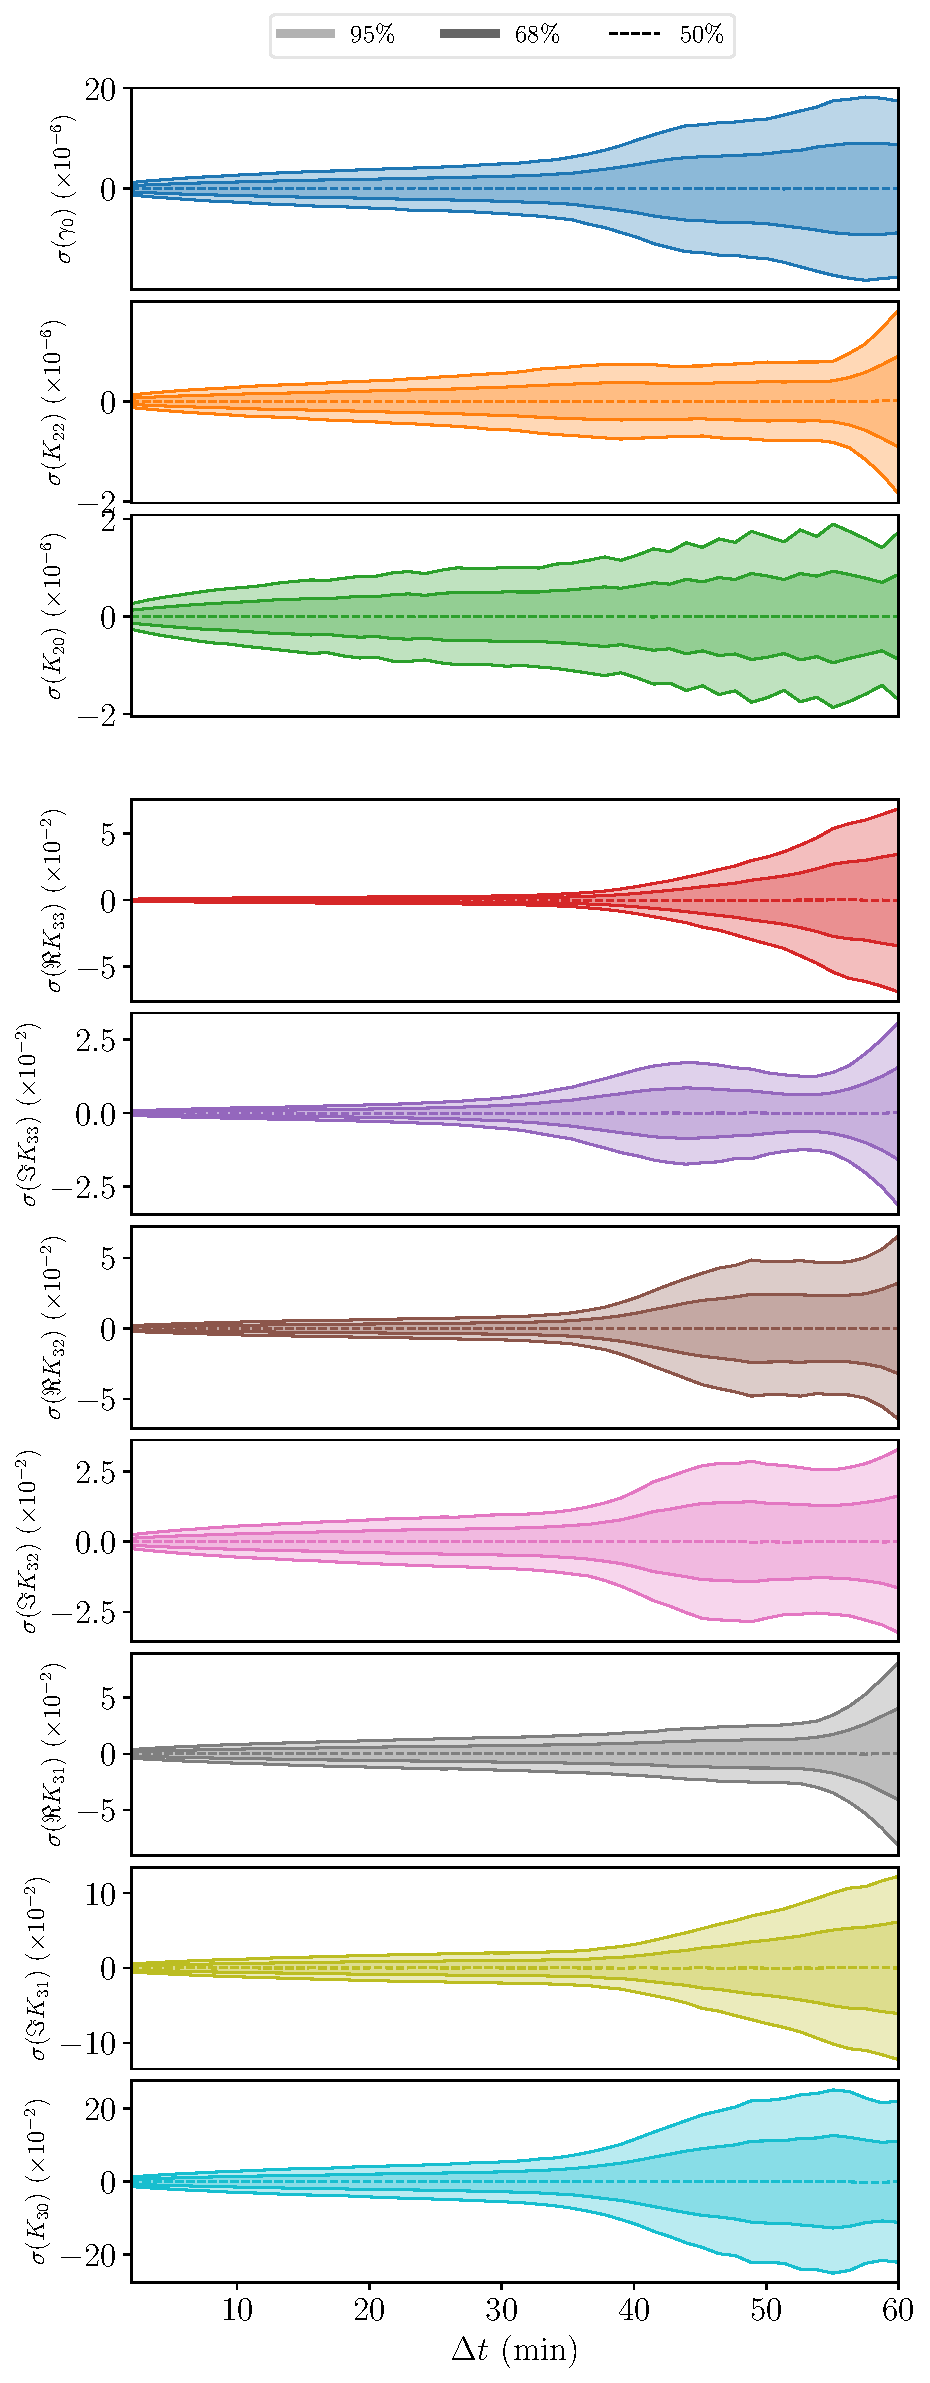
\includegraphics[height=0.89\textheight]{figs/scan-cadence.pdf}
  \caption{1- and 2-$\sigma$ confidence intervals for the first-order parameter posteriors (\textit{top}) and second-order parameters (\textit{bottom}) as a function of observational cadence $\Delta t$ The reference cadence is 2 minutes. The red vertical lines indicate when $\sigma = 0.01$.}
  \label{fig:scan-cadence}
\end{figure}

Figure \ref{fig:scan-cadence} displays little dependence of uncertainty on cadence ($\Delta t$) for $\Delta t \lesssim 40$ min. We also see flaring of uncertainty for very large cadence, largely driven by the paucity of data points. However, uncertainty dramatically increases for many parameters at about $\Delta t = 40$ min, a time scale which is likely characteristic of the asteroid system. We name this rough cadence limit $T_\text{cad}$.

By dimensional analysis, we expect $T_\text{cad}$ to be a function of two dynamical time scales of the system: the rotational period of the asteroid $P$ and the time spent near perigee $T_p$. The latter can be estimated by the unitless combination
\begin{equation}
  T_p \sim \frac{r_p}{v_\infty}\brackets{2\frac{M}{r_pv_\infty^2}+1}^{-\frac{1}{2}}
  \label{eqn:tp}
\end{equation}
which is the ratio of the perigee radius to velocity at perigee. The exact choice of the formula of $T_p$ not obvious, and alternatives to equation \ref{eqn:tp} are possible. For the simulated asteroid, $P = 9$ hr and $T_p = 42$ min by this definition. Immediately we see $T_p \approx T_\text{cad}$, but this is not necessarily significant because $T_p$ is an estimate.

Which of $P$ and $T_p$ is more important to the determination of $T_\text{cad}$ is assessed in appendix \ref{app:cadence-tests}.

Figure \ref{fig:scan-cadence} shows that as long as $\Delta t < T_\text{cad}$ is achieved, the influence of cadence on $\sigma$ is minimal. However, it is generally better to have short cadence when possible.



\subsection{Perigee gap}
\label{sec:scan-gap}
In certain negative circumstances, spin data might not be able to be captured for a close encounter at perigee. The asteroid might dip below the horizon, or it might pass too close to the sun to be observed. Generally, angular velocity data can be collected when the asteroid is distant from the central body, where torque is low. The angular velocity evolution here is dominated by torque-free precession dictated by the moment of inertia components. so that zero-torque data can still be used to fix $K_{20}$ and $K_{22}$ \cite{MOSKOVITZ2020113519}. However, $K_{3m}$ are not extractable from precession data alone. We are therefore curious as to how our posterior uncertainties change due to lack of data during the encounter perigee.

To test this, we mask the perigee of the counter by removing data within time $T$ of the perigee, where $T$ ranges from 0 to 3 hours. To prevent lack of precision on $K_{\ell m}$ induced by lower amounts of data for high $T$, we always cut 3 hr$-T$ from the data set, half from the beginning and half from the end, so that each data set produced for all $T$ has the same length of data before and after the perigee. We then fit the same asteroid model to the cut data for all $T$ and plot posterior uncertainties $\sigma$ in figure \ref{fig:observation-gap}.

\begin{figure}
  \centering
  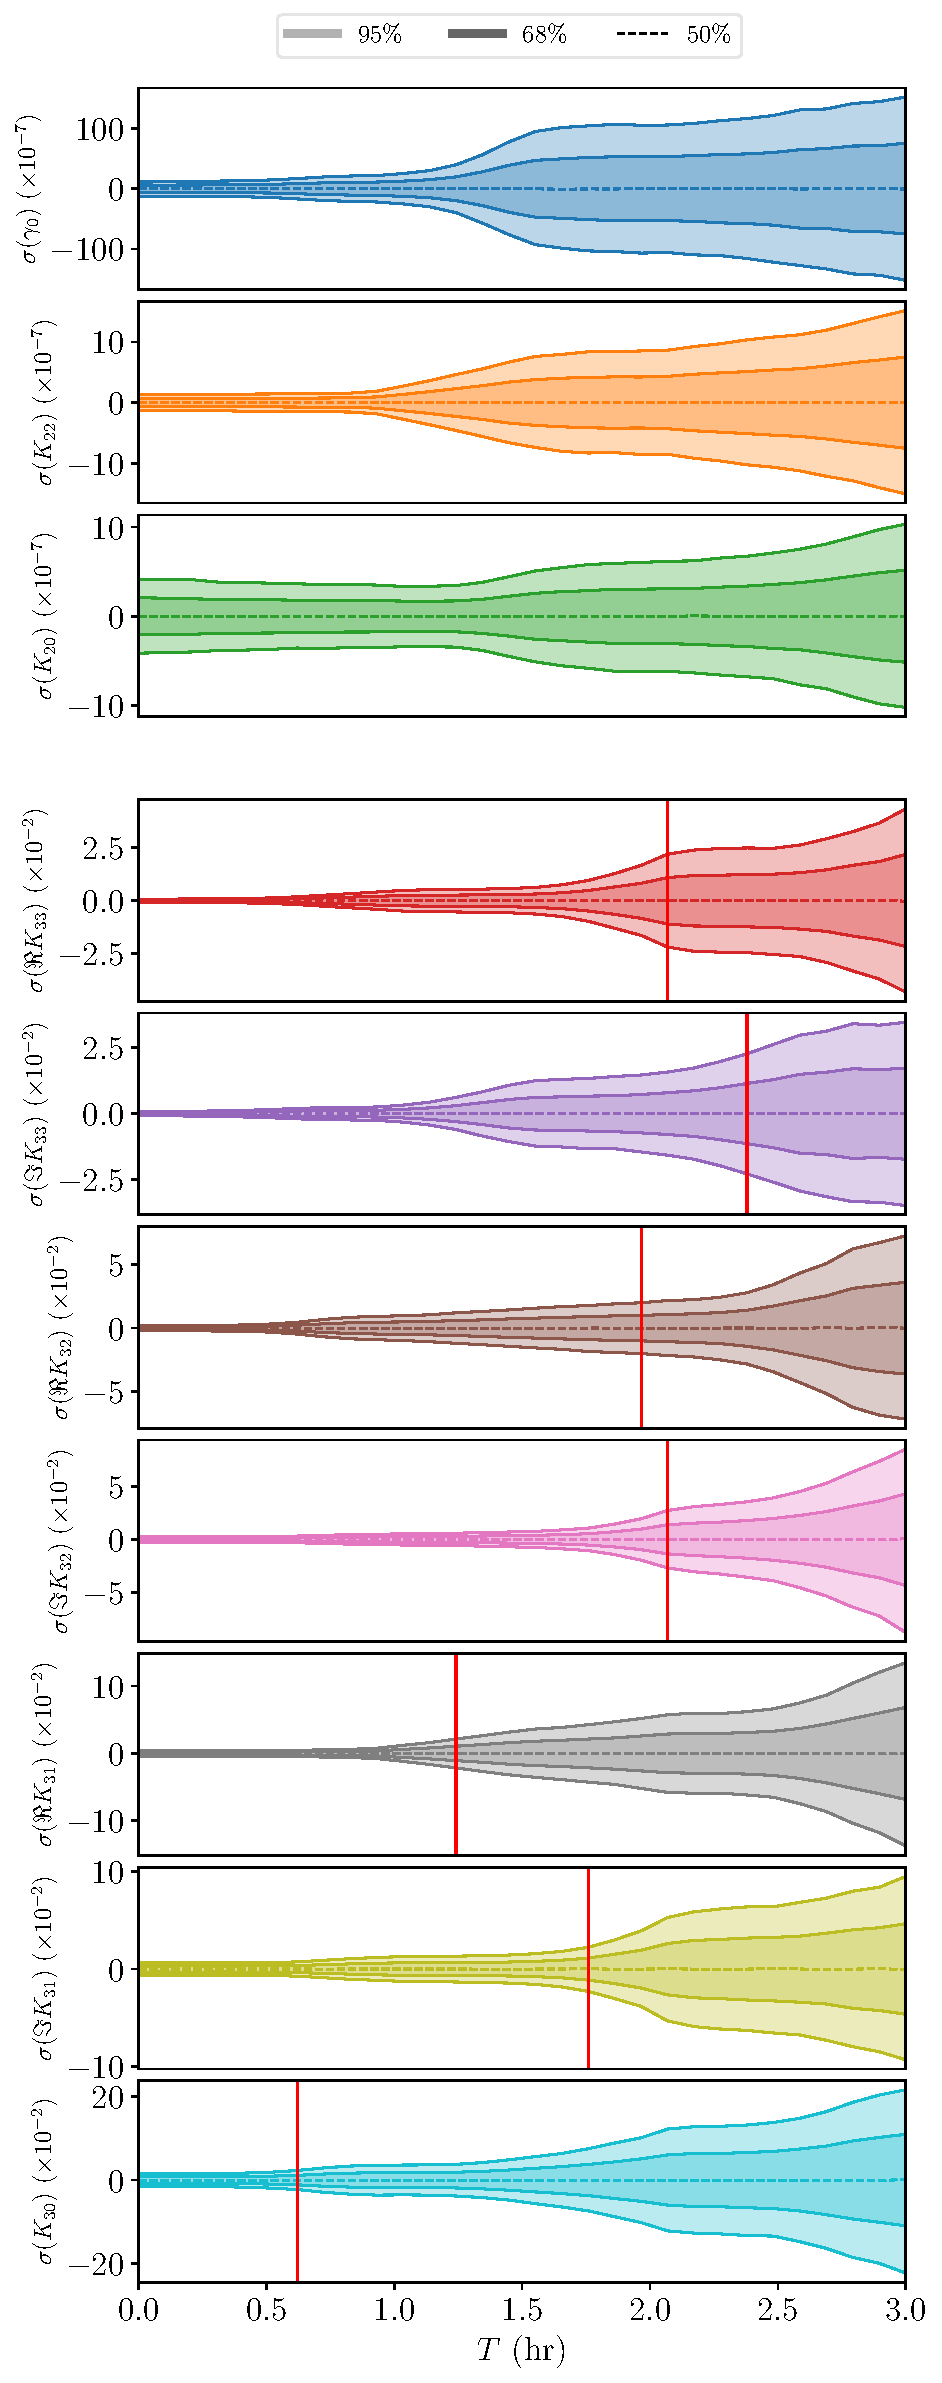
\includegraphics[height=0.89\textheight]{figs/observation-gap.pdf}
  \caption{1- and 2-$\sigma$ confidence intervals for the first-order parameter posteriors (\textit{top}) and second-order parameters (\textit{bottom}) as a function of a data gap of width $T$ at perigee. The red vertical lines indicate when $\sigma = 0.01$.}
  \label{fig:observation-gap}
\end{figure}

Since torque is highest at perigee, we expect that region of the data to contain the most information about $K_{\ell m}$, and therefore that uncertainty should increase monotonically with $T$, which is seen in figure \ref{fig:observation-gap}. We also see that the first-order parameters are not as sensitive to $T$ as the second-order parameters, because $K_{2m}$ are additionally constrained by torque-free precession after perigee.

Most parameters show dramatically increased uncertainty in the $T \sim 1-2$ hr range. This cutoff is likely determined by the orbital elements of the encounter, which control how much time the asteroid spends in the high-torque region. On the other hand, none of the uncertainties increase noticeably for $T < 30$ min. Thirty minutes of dropped data is equivalent to fifteen dropped points for the simulated cadence of $\Delta t = 2$ minutes, showing that many data points can dropped from the data set at perigee before the uncertainty starts to increase.

Qualitatively, \ref{fig:observation-gap} shows similar dependence of $\sigma$ on $T$ as \ref{fig:scan-cadence} showed for $\sigma$ on cadence $\Delta t$. They also have quantitatively the same cutoff of 30 min before uncertainty is markedly affected. This suggests that the factors that govern uncertainty due to cadence and uncertainty due to lack of data at perigee are the same.


\subsection{Initial spin pole}
\label{sec:scan-spin}

The tidal torque experienced by the asteroid is affected by the initial direction of asteroid spin $\bm \omega_0$ both because spin sets the initial asteroid orientation (up to $\gamma_0$) and because of the spin-dependence of the rotational equations of motion (equation \ref{eqn:omega-eom}). As an example, in section \ref{sec:tidal-torque}, we noted that $\bm \omega_0 \parallel \unit Z$ leads to $\bm \tau = 0$ and therefore all parameters are unconstrained.

In figure \ref{fig:scan-spin}, we display 1-$\sigma$ uncertainties for all parameters as a function of the direction of $\bm \omega_0$, mapped onto the sky in the inertial frame. Our samples for $\bm \omega_0$ were laid out on a Fibonacci sphere to ensure they were evenly spaced (marked in figure \ref{fig:scan-spin-avg}). To highlight common features across the parameters, we also display the average 1-$\sigma$ sensitivity in figure \ref{fig:scan-spin-avg}. The average is weighted such that the uncertainty map for each parameter contributes an equal amount
(the weight of each map is set to one-tenth of the map's mean). This average map is presented in two different projections to allow data at $\unit Z$ to be read.

\begin{figure*}
  \centering
  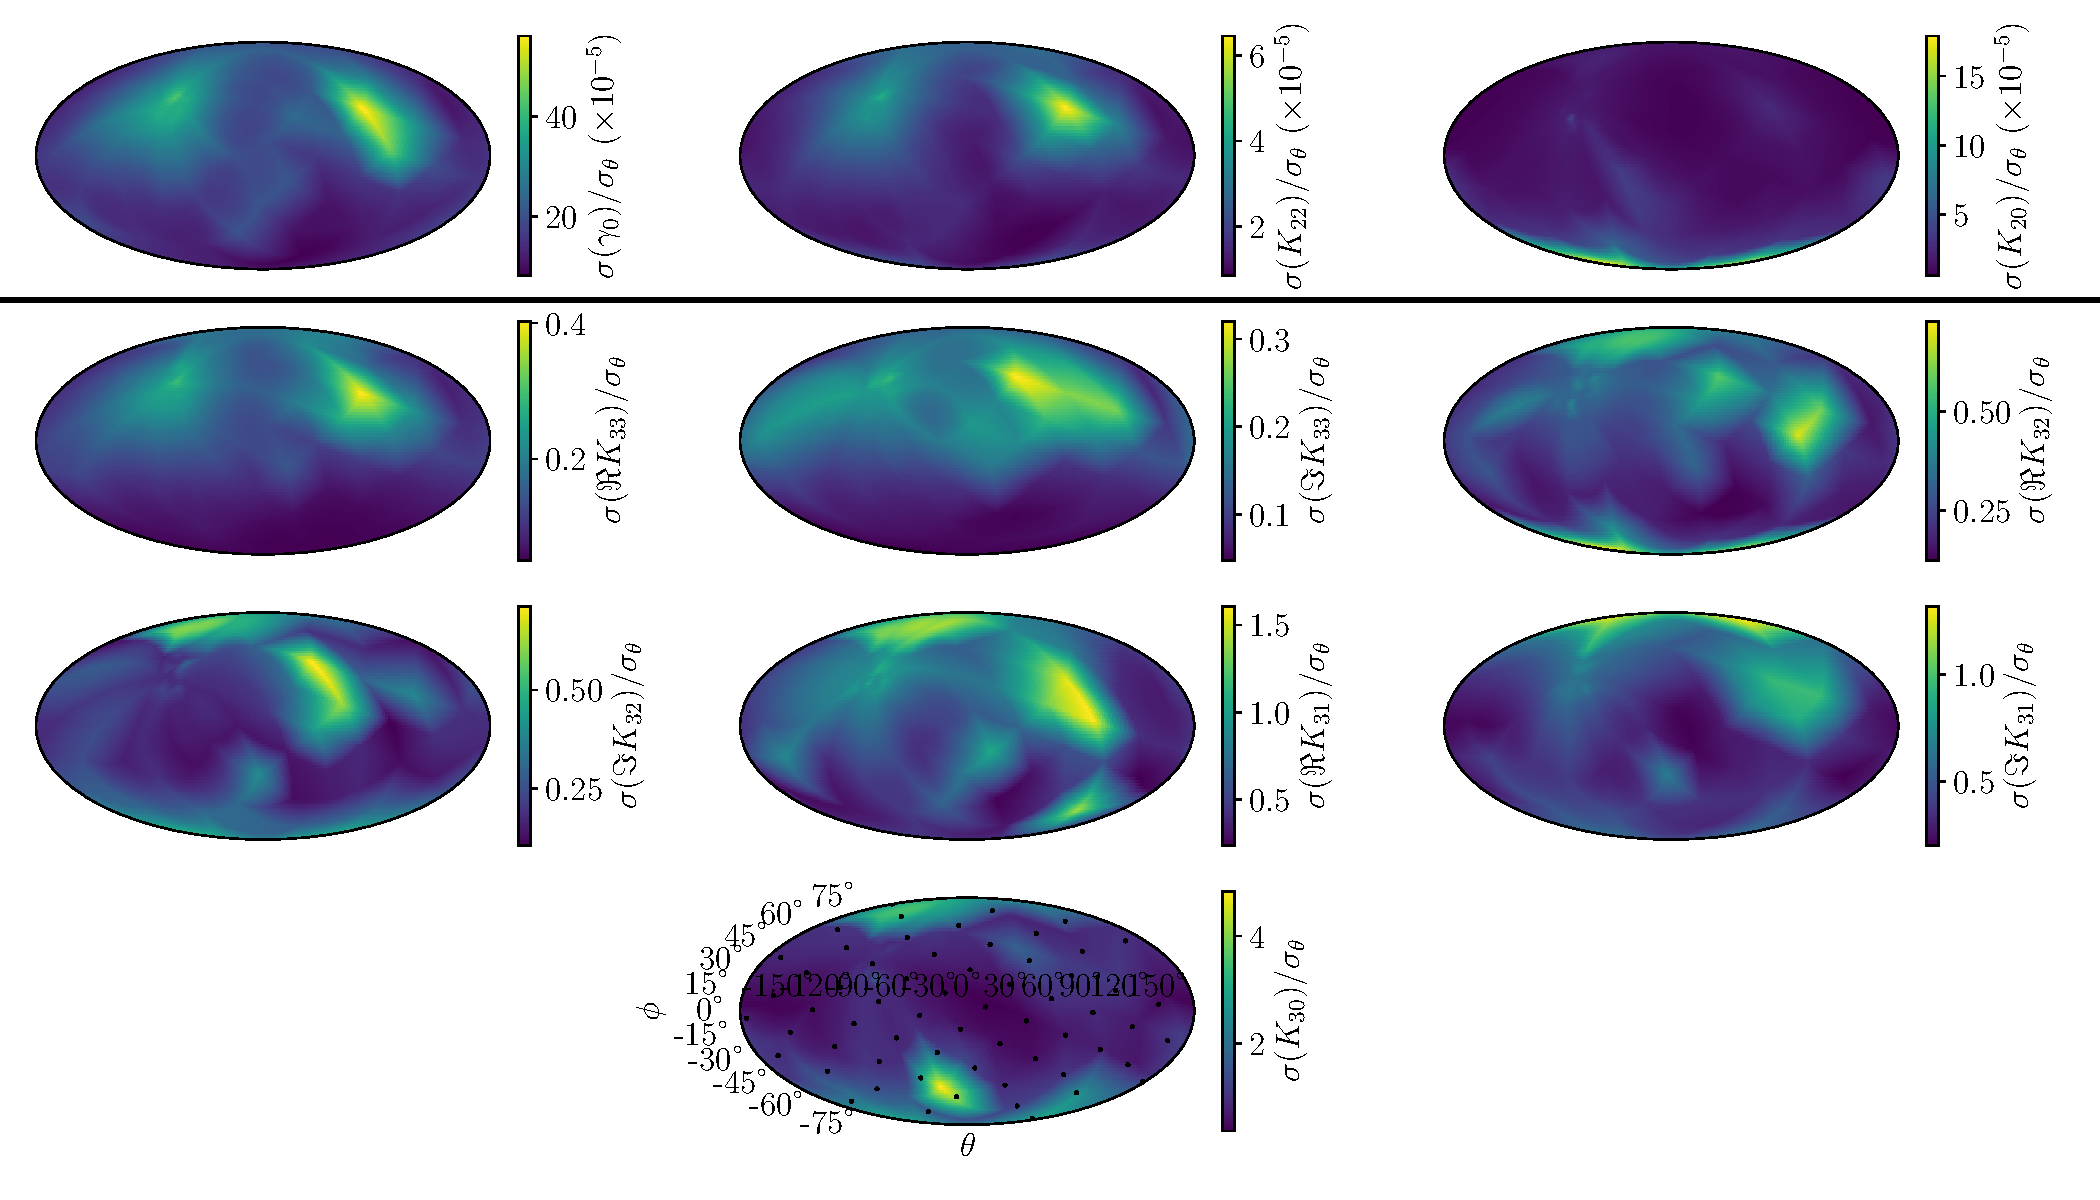
\includegraphics[width=\textwidth]{figs/spin-pole.pdf}
  \caption{$1-\sigma$ uncertainties for the first-order parameters (\textit{top}) and second-order (\textit{bottom}) as a function of the initial direction of spin in the inertial frame. All maps are made in the Mollweide projection and shown in the inertial $\unit X-\unit Y-\unit Z$ frame. The orange star indicates the reference spin pole. The red contours enclose regions where $\sigma \geq 0.01$.}
  \label{fig:scan-spin}
\end{figure*}

\begin{figure*}
  \centering
  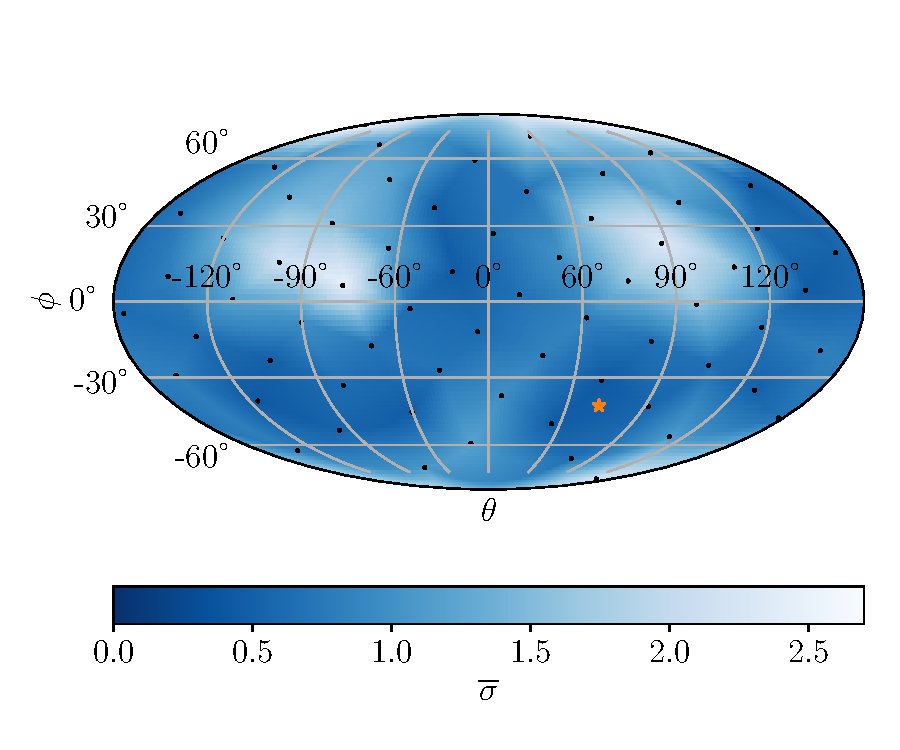
\includegraphics[width=0.45\textwidth]{figs/spin-pole-avg-mollweide.pdf}
  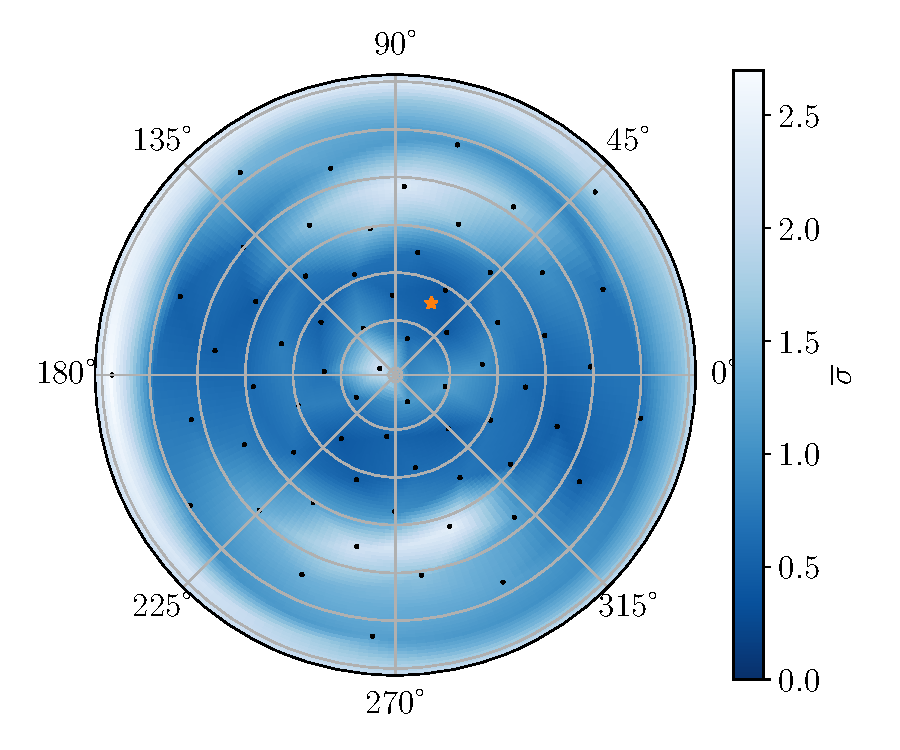
\includegraphics[width=0.45\textwidth]{figs/spin-pole-avg-polar.pdf}
  \caption{The weighted average of the uncertainties shown in figure \ref{fig:spin-pole}, in Mollweide (\textit{left}) and polar (\textit{right}) projections. See text for a description of how the average was computed. Black dots indicate the locations of sample spin poles, and the orange star indicates the reference spin pole.}
  \label{fig:scan-spin-avg}
\end{figure*}

The characteristics of tidal torque discussed in section \ref{sec:tidal-torque} indicate that certain alignments of the body-fixed frame to the inertial frame lead to special conditions on torque: $\bm z \parallel \unit Z$ and $\bm z \parallel \unit Y$ at perigee lead to $\bm \tau \parallel \unit z$ to first order, and $\bm \tau \parallel \unit X$ at perigee leads to $\bm \tau = 0$ to first order. We relate this to the initial direction of $\bm \omega_0$, via the crude assumption that $\bm \tau$ is small until perigee. Then, since $\bm \omega_0 \parallel \unit z$ by assumption that the asteroid is not tumbling, we have that $\bm \omega_0 \parallel \unit Y$ and $\bm \omega_0 \parallel \unit Z$ lead to $\bm \tau \parallel \unit z$, and $\bm \omega_0 \parallel \unit X$ leads to $\bm \tau = 0$.

Figure \ref{fig:scan-spin-avg} shows area of increased uncertainty for $\bm \omega_0 \parallel \unit Z$ and $\bm \omega_0 \parallel \unit Y$, but not the $\unit X$ case. This indicates that $\bm \tau \parallel \unit z$ causes increased uncertainty. Physically, $\bm \tau \parallel \unit z$ only changes an asteroid's rotational period and does not cause it to tumble, eliminating the ability to discern moment of inertia ratios from zero-torque precession after the flyby. Also, $\tau_z$ is small and affected by fewer parameters than $\tau_x$ or $\tau_y$.  Both of these are reasons why $\bm \tau \parallel z$ might inhibit precise fits to spin data. If $\bm \tau = 0$ to first order, then second-order $\tau$ and non-perigee $\bm \tau$ will dominate, and these may indeed induce precession.

It is important to note, however, that uncertainty does not vary by much more than a factor of two outside the imprecise regions of $\bm \omega_0 \parallel \unit Z$ and $\bm \omega_0 \parallel \unit Y$, though these regions are wide for some parameters. Within the imprecise regions, uncertainty can grow up to four times the uncertainty at other $\bm \omega_0$ values, and possibly higher. The trends for are roughly consistent across parameters (figure \ref{fig:scan-spin}), leading to clearly visible imprecise regions in figure \ref{fig:scan-spin-avg}


\subsection{Oblateness}
\label{sec:scan-oblateness}

In all the above studies, we assumed a spherical planet ($J_{\ell m} = 0$ for $\ell \geq 1$). By assumption that $\mu_M \gg \mu_m$ (so that the asteroid orbit's focus is the center of mass of the central body), we have $J_{1m} = 0$. The effect of oblateness, then, is limited to the $J_{2m}$ terms, and therefore damped by a factor of $(a_M / D)^2$. We expect these parameters to have little effect on the asteroid.

Here, we define oblateness as $\epsilon = (I_z - I_x)/(\mu_M R_M^2)$, where  $I_{x,y,z}$ are the central body moments of inertia along the principal axes, and $I_x = I_y$. $R_M$ is the true radius of the body (not $a_M)$. Note that $J_{\ell m}$ is defined in equation \ref{eqn:jlm} with respect to the asteroid orbit, not the principal axes of the central body. But for an equatorial orbit, the principal axes coincide with the asteroid orbit frame and we may express $\epsilon$ simply in terms of $J_{\ell m}$ as $\epsilon = -2J_{20}$ and $J_{22} = 0$. (Some sources such as Ref.~\cite{paterLissauer2015} take this definition of $\epsilon$ as their definition of $J_{20}$). Given this conversion between $\epsilon$ and $J_{20}$, we analyze posterior uncertainty $\sigma$ of the first-order parameters as a function of $\epsilon$ across a reasonable range ofittedf oblatenesses based on those of Solar System planets \cite{paterLissauer2015}. These uncertainties are shown in figure \ref{fig:scan-oblateness}.

\begin{figure}
  \centering
  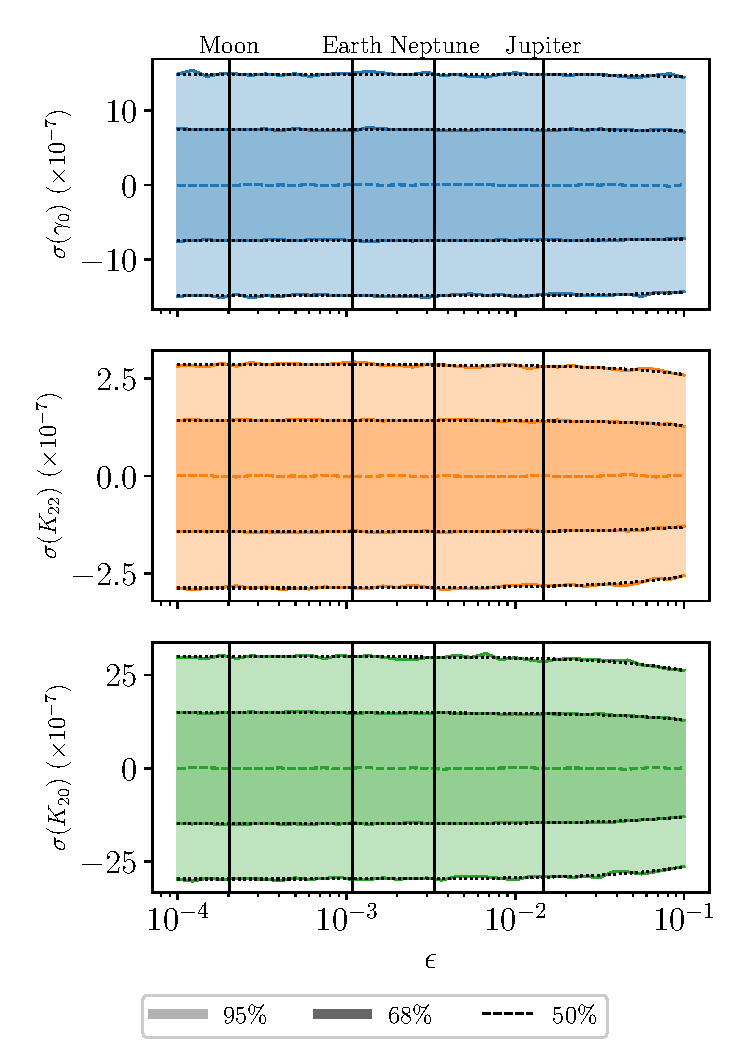
\includegraphics[width=0.88\columnwidth]{figs/oblateness.pdf}
  \vfill
  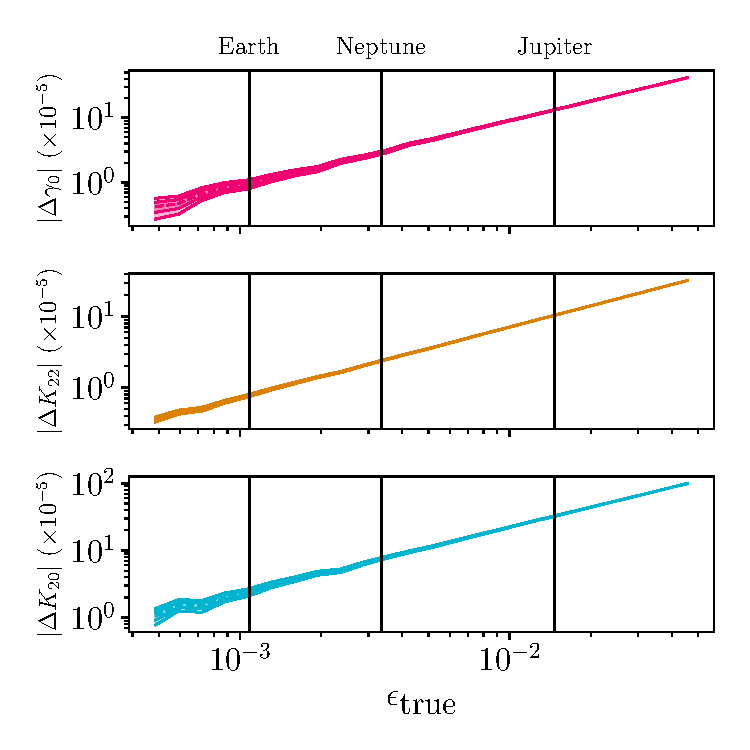
\includegraphics[width=0.88\columnwidth]{figs/oblateness-differ.pdf}
  \caption{\textit{Left}: 1- and 2-$\sigma$ confidence intervals for the first-order parameter posteriors as a function of oblateness $\epsilon$ . Linear best fit lines to $\sigma$ (black, dotted) are plotted. \textit{Right}: The deviation of posterior mean extracted from a zero-oblateness model from the true parameters given a model with oblateness $\epsilon \neq 0$. Also shown in both figures are the oblatenesses of reference Solar System bodies.}
  \label{fig:scan-oblateness}
\end{figure}

Figure \ref{fig:scan-oblateness} (top pane) demonstrates a small dependence of $\sigma$ on oblateness $\epsilon$, but the effect is far from the effect of other factors studied above. Most Solar System bodies do not reach the oblateness necessary to significantly increase precision on the first-order parameters. The linear best-fit lines match the data well, and they have slope of $(\Delta \sigma / \sigma_{\epsilon=0}) / \Delta \epsilon = -0.26$ for $\gamma_0$, $-0.94$ for $K_{22}$, and $-1.2$ for $K_{20}$. Other parameters $K_{3m}$ likely depend on oblateness similarly, but fitting these parameters is computationally more expensive.

Note that if a flyby is executed around one of the non-Earth objects noted in figure \ref{fig:scan-oblateness}, $a_M$ and $\mu_M$ will change in addition to $\epsilon$. These two parameters do affect the precision of the fit parameters, so the figure does not state that encounters with other bodies have the same precision as encounters with Earth; only that the difference in oblateness between the two bodies is of little concern.

Given the small effect of $\epsilon$ on $K_{\ell m}$, it might be tempting to neglect the effect of planetary oblateness when fitting $K_{\ell m}$ to data. However, the bottom pane of figure \ref{fig:scan-oblateness} demonstrates that this is not valid. This figure displays $K_{\ell m}$ as extracted by a fit assuming $\epsilon = 0$, but run on data generated by assuming nonzero $\epsilon$. The difference between the posterior mean $K_{\ell m}$ and true $K_{\ell m}$ are shown. Posterior uncertainties are also shown as bands. The figure shows that even for low (Moon-scale) oblateness, the fit results are inconsistent with the true $K_{\ell m}$ values, since $|\Delta K_{\ell m}| = 0$ is not contained in the 2-$\sigma$ band. This effect is much worse for large oblateness, growing to a difference on the order of $10^{-2}$ between the true and fit parameters for large oblateness. Therefore, accurately modeling oblateness to high precision is essential for accurate estimation of fit parameters. For non-equatorial orbits, with $J_{22} \neq 0$, we also expect $J_{22}$ to affect the accuracy of the fit results to a similar degree, so it is also vital to use the correct asteroid orbital plane.

Note that $J_{20}$, the parameter studied in this section, has a slightly more general definition than oblateness. If the planet has a moon, the integral defining $J_{20}$ (equation \ref{eqn:jlm}) can be extended to include this extra mass, including it in $J_{20}$. Since $J_{20}$ is a second moment, this effect is magnified for large distances of the mass from the central body center of mass (though the effect is not quite quadratic because $a_m$ also increases for large distances). This process is only valid when the asteroid never passes closer to the central body than the moon.

As an order-of-magnitude estimate for this effect, two spherical masses with masses and radii of Earth and the Moon, separated by one Lunar distance, and both lying in the orbital plane has a combined $J_{20} = 0.25$. Extrapolating posterior uncertainty by the slopes of the best fit lines given earlier, this represents a decrease in $\sigma(K_{2m})$ by a factor of about one quarter.

This analysis suggests that large moons such as ours can improve fit quality, but further study of this effect is beyond the scope of this paper. Without a moon to inflate the oblateness of the central body, planetary oblateness does not significantly improve posterior uncertainty. However, correct representation of oblateness is essential to correctly estimate $K_{\ell m}$.



\subsection{Rotational period}
\label{sec:scan-period}

The final encounter parameter we study is the initial rotational period of the asteroid $P_\omega$. The dynamical time scales $r_p/v_\infty$ and $\mu_m / (r_p v_\infty)$ have already been mentioned and the ratio between them and $P$ in principal may affect the posterior uncertainty $\sigma$. In figure \ref{fig:scan-period}, we show $\sigma$ as a function of $P_\omega$ for a range of periods typical of NEOs.

\begin{figure}
  \centering
  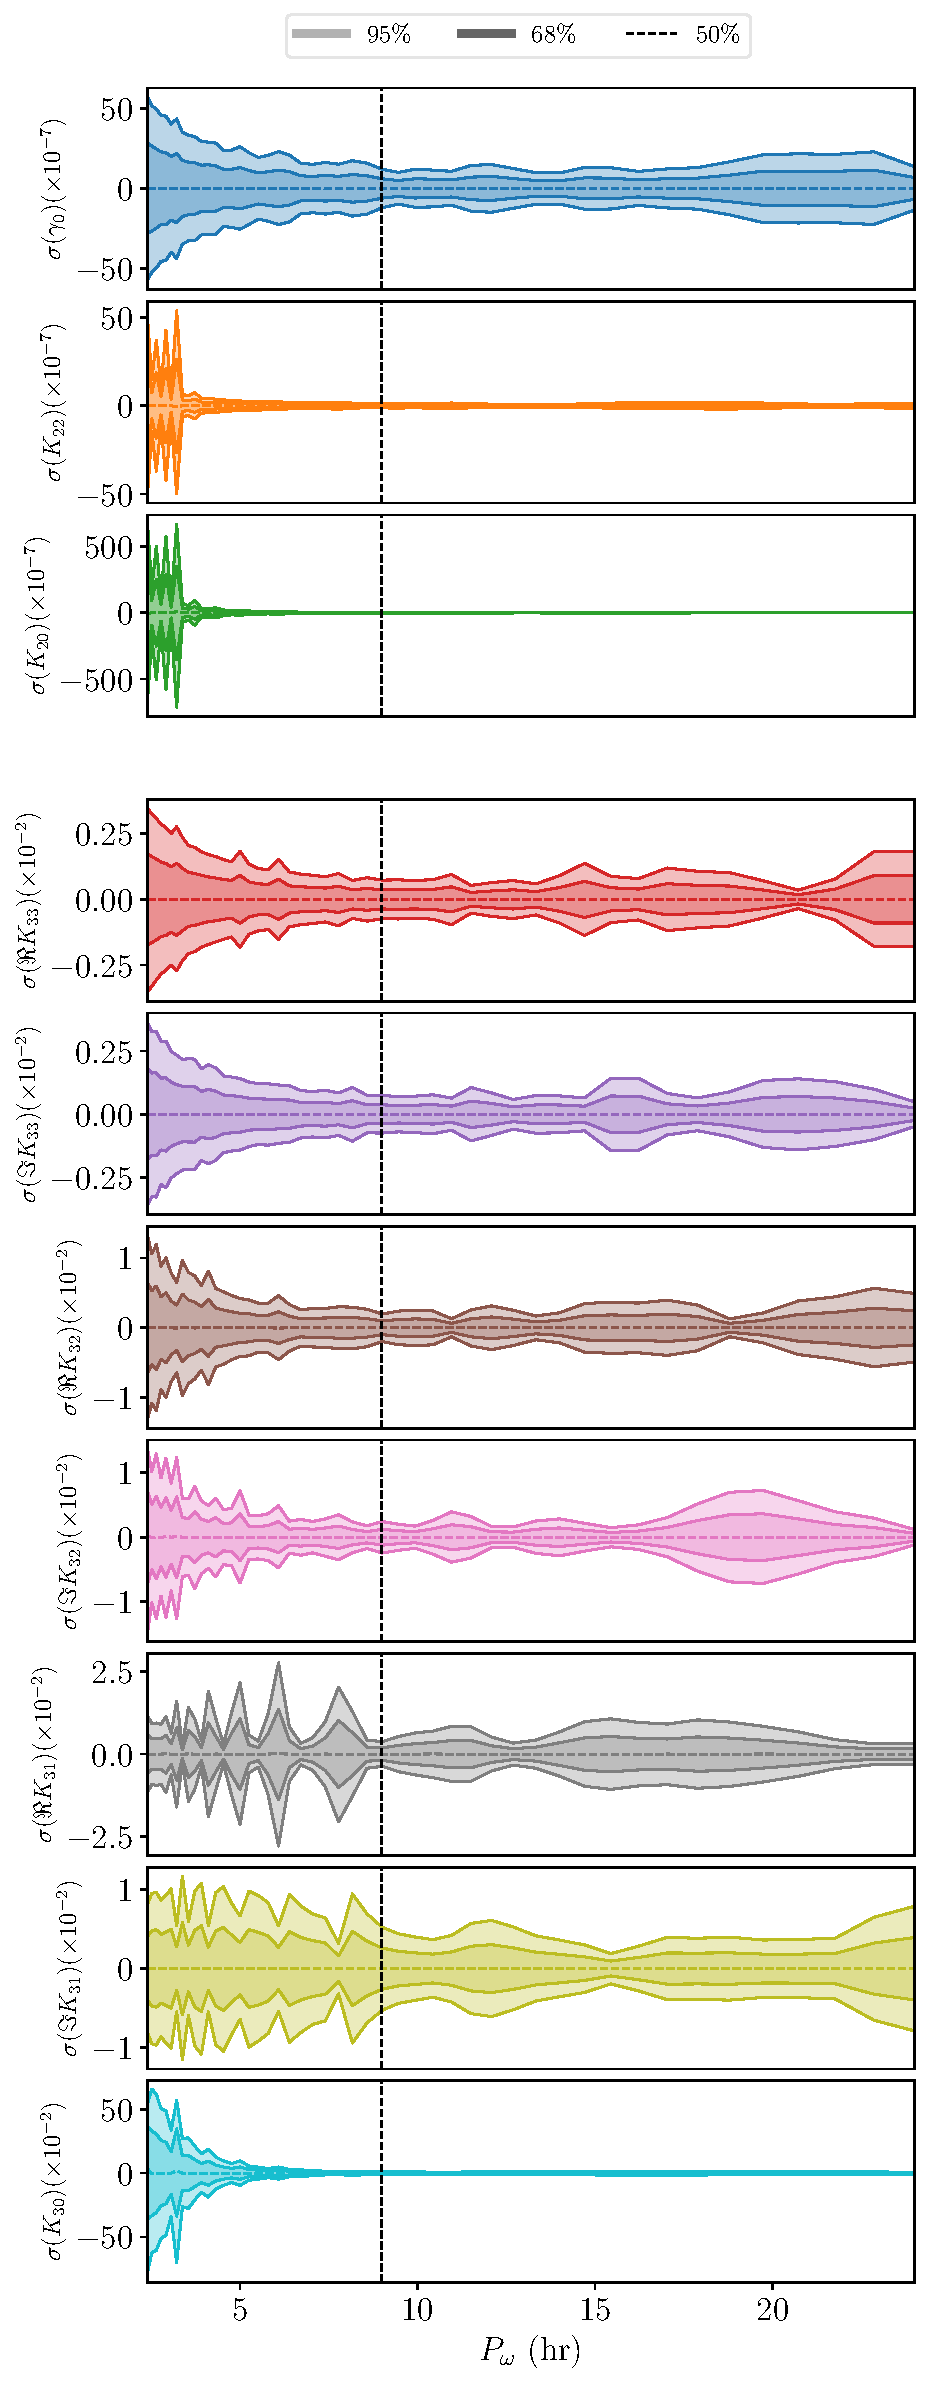
\includegraphics[height=0.89\textheight]{figs/scan-period.pdf}
  \caption{1- and 2-$\sigma$ confidence intervals for the first-order parameter posteriors (\textit{top}) and second-order parameters (\textit{bottom}) as a function of initial rotational period $P$. The reference value of 9 hr is shown as a vertical dotted line. The red vertical lines indicate when $\sigma = 0.01$.}
  \label{fig:scan-period}
\end{figure}

Like figure \ref{fig:scan-vex}, depicting the dependence of $\sigma$ on $v_\infty$, figure \ref{fig:scan-period} shows small-scale variation in uncertainty due to the fact that varying the initial period changes the value of $\gamma$ at perigee, which affects uncertainty to a factor of about two. But a large-scale trend is also visible in many parameters. $K_{20}$ and $K_{22}$ show very large uncertainty for low $P_\omega$ because these asteroids do not tumble after perigee, and tumbling after the perigee allows better refinement of the $K_{2m}$ parameters. 

We expect that quickly rotating asteroids would not tumble because, for small $P_\omega$, the dynamical variables $\bm D$, $\bm \omega$, $\alpha$, $\beta$, and which affect $\bm \tau$ vary much smaller than $\gamma$. Approximating each variable as constant over one full rotation of $\gamma$, we can integrate the first order contribution of $\bm \tau$ over $\gamma \in (0, 2\pi)$ and we see that each rotation has zero average first-order torque. Since the first-order torque over each rotational period cancels out, there is no secular torque to force the asteroid to tumble. However, this effect does not apply to the second-order parameters, since the integral over the second-order term of $\bm \tau$ does not vanish, as seen in the figure.

Another feature of figure \ref{fig:scan-period} is that $K_{\ell 0}$ is more uncertain at low $P_\omega$ than the other parameters. This is most visible in the figure for $K_{30}$. The cause of this is likely that $K_{\ell 0}$ cannot contribute to $\tau_z$ as shown in equation \ref{eqn:tidal-torque}. We already discussed that asteroids with $P_\omega$ large do not tumble, and since $\tau_x$ and $\tau_y$ are what induces tumbling, the most observable component of torque is therefore $\tau_z$, which $K_{\ell 0}$ don't affect.

The most severe effect of period on $\sigma$ is in the low-period regime ($P_\omega \lesssim 5$ hr), but in this case, the most strongly affected parameters are $K_{2m}$, which are generally known better than $K_{3m}$. The effect on the imprecise parameters $K_{3m}$ is small, except for $K_{30}$. It therefore seems as though small-period asteroids are still candidates for observation, although high-period asteroids still have better uncertainty.


\section{Density distributions}
\label{sec:distros}

Hitherto, we have only discussed the density moments $K_{\ell m}$ of the asteroid rather than the true density distribution $\rho(\bm r)$. This is because only the density moments are observable by tidal torque interactions. However, by making assumptions about the density distribution, we can nevertheless estimate $\rho(\bm r)$ from $K_{\ell m}$.

In this section, we outline three different assumptions which yield different types of density distributions for the same $K_{\ell m}$. One of them can be chosen, or a fourth created, depending on what features are desired to be represented in the density distribution. All three of these models assume that the asteroid shape is known (for example, by light curve or radar data). Uncertainty on this shape estimate is assumed to be small. The models then produce a density distribution $\rho(\bm r)$ with uncertainty from $K_{\ell m}$ propagated to uncertainty in $\rho$.

Note that, since the overall mass of the asteroid is not observable from tidal torque, we do not expect to measure $\rho$ in an absolute sense. Only the differences in $\rho$ across the body are measurable.

In section \ref{sec:general-density}, we describe the general form our three models must take. Then we lay out each individually and compare them in section \ref{sec:density-compare}. In appendix \ref{app:find-surface}, we do not assume that the asteroid shape is known and instead assume that the density is constant. This allows us to compute the asteroid shape from $K_{\ell m}$.


\subsection{General density model design}
\label{sec:general-density}

To set the shape of the asteroid, we assume that an indicator function $\mathds{1}(\bm r)$ has been determined such that $\mathds{1}(\bm r) = 1$ inside the asteroid and 0 outside, where $\mathds{1}(\bm r)$ is defined in some frame whose orientation with respect to Earth is known. Since the asteroid rotates around its center of mass during observations, we assume that the location of the center of mass is also known in this frame, so that we can set it to be the origin.

We define a new coordinate system, the ``hybrid frame,'' which coincides exactly with the initial orientation of the asteroid assuming that the fit result for $\gamma_0$ is perfectly accurate. The orientation of the hybrid frame with respect to the inertial frame is therefore exactly known, so that $\mathds{1}$ is also exactly in the hybrid frame, and the $K_{\ell m}$ components are known in the local frame which aligns with the hybrid frame up to uncertainty in $\gamma_0$. We will solve for $\rho(\bm r)$ in the hybrid frame given fit results $K_{\ell m}$ and the known $a_m$.

The density moments defined in equation \ref{eqn:klm} are not linear in $\rho(\bm r)$, but we may fix $a_m$ at the value assumed during the fit, removing the non-linearity induced by division by $a_m$. Furthermore, since the system is independent of the total asteroid mass, we set $\mu_m$ equal to an arbitrary constant which makes equation \ref{eqn:klm} linear in $\rho(\bm r)$. Similarly, the form of equation \ref{eqn:am} guarantees that $a_m^2$ is linear in $\rho(\bm r)$. Equation \ref{eqn:am} and equation \ref{eqn:klm} applied to $K_{00}=1$ can be used to enforce the choices of $\mu_m$ and $a_m^2$.

Suppose that we restrict the number of degrees of freedom of $\rho(\bm r)$ from infinity to $m$ by explicitly defining some function $\rho(\bm r, \bm D)$ for an $m$-dimensional vector $\bm D$ which controls the free parameters of $\rho$. We will leave the explicit definition of $\rho(\bm r, \bm D)$ to the model descriptions below, but for now we assume that $\rho$ is linear in $\bm D$; i.e.,
\begin{equation}
  \rho(\bm r, \bm D) = \bm B(\bm r) \cdot \bm D
  \label{eqn:density-distro}
\end{equation}
for a $m$-dimensional vector $\bm B(\bm r)$. Thus, the defining equations of $a_m^2$ and $K_{\ell m}$ represent a linear function that give the parameters in terms of $\bm D$. We further assume that the model describes a way to reverse this equation, to write
\begin{equation}
  \bm D = A \bm K
  \label{eqn:density-model}
\end{equation}
where $A$ is a matrix. Here, we have arranged $a_m^2$ and the known components of $K_{\ell m}$ into a vector $K$, which we say has $n$ dimensions. The order of this arrangement is irrelevant, as long as it is kept consistent.

To propagate uncertainties from $\bm K$ to $\bm D$ and therefore $\rho(\bm r)$, we first need the covariance matrix $\Sigma_K$ for $\bm K$. First, assume that the hybrid frame is offset from the local frame by some small angle $\Delta \gamma$, which results from uncertainty in $\gamma_0$. Then
\begin{equation}
  K_{\ell m}^\mathrm{hybrid} = e^{-im\Delta \gamma}K_{\ell m}^\mathrm{local}.
  \label{eqn:local-to-hybrid}
\end{equation}
Since $K_{\ell m}^\mathrm{local}$ was obtained by an MCMC fit, a large set of posterior-distributed samples are available for $\Delta \gamma$ and $K_{\ell m}^\mathrm{local}$, and the covariance matrix $\Sigma_K$ can be computed statistically by applying equation \ref{eqn:local-to-hybrid} to the samples. Then, propagation of uncertainty guarantees that the covariance matrix of $\bm D$ is $\Sigma_D = A \Sigma_K A^T$
and the density distribution and uncertainty on density distribution are equal to
\begin{equation}
  \rho(\bm r) = \bm B(\bm r)^T A\bm K \qquad \sigma^2_\rho(\bm r) = \bm B(\bm r)^T A \Sigma_K A^T \bm B(\bm r).
  \label{eqn:unc-rho}
\end{equation}

The job of a model is therefore to restrict the space of valid density distributions by defining the $m\times n$-dimensional constant matrix $A$ and the $m$-dimensional vector $\bm B(\bm r)$ such that equations \ref{eqn:density-model} and \ref{eqn:density-distro} are true. Then the density distribution and its uncertainty are given by equation \ref{eqn:unc-rho}.



\subsection{The Likelihood model}
For the likelihood model, we restrict the degrees of freedom of $\rho(\bm r)$ by defining a likelihood function $\mathcal{L}$ on the density distribution, and choosing the one distribution which maximizes likelihood and exactly reproduces $\bm K$. This likelihood should not be confused with the likelihood of equation \ref{eqn:log-likelihood}, which was a function of the spin data, not the density distribution. The choice of the density $\mathcal{L}$ is arbitrary, but the linearity of the model design outlined in the previous section will require an uncorrelated Gaussian likelihood.

To employ this likelihood method, we divide the asteroid into a square grid of $m \gg n$ elements, each of which is assumed to have uniform density $\rho_0$ plus some deviation $D_i$, where $\rho_0$ is constant across the asteroid. This defines the model function $\bm B(\bm r)$, which is zeroed in all components except for the $i$th, where $i$ is the index of the grid element that contains $\bm r$.

We use a likelihood of 
\begin{equation}
  \mathcal{L}(\bm D) = \prod_{i=1}^m \frac{1}{\sqrt{2\pi \sigma^2}} \exp\parens{-\frac{D_i^2}{2 \sigma^2}}
\end{equation}
with free parameters $\mu$ and $\sigma$. These parameters do not affect the location of the maximum, so we do not define them. Given this likelihood, the log likelihood is proportional to $-|\bm D|^2$. Minimizing the norm of $\bm D$ is therefore equivalent to finding the maximum likelihood.

Putting aside the problem of minimizing the norm for a moment, we use the linearity of equations \ref{eqn:klm} and \ref{eqn:am} to write $\bm K = M \bm D$, where the $i$th entry of every row of the $n\times m$ matrix $M$ is the integral presented in equation \ref{eqn:jlm} or \ref{eqn:am}, evaluated over the $i$th finite element. We want to solve $\bm K = M \bm D$ for $\bm D$ to match equation \ref{eqn:density-model}, which we do via the Moore-Penrose inverse. Since $m>n$, the Moore-Penrose inverse of $M$ is
\begin{equation}
  A=M^+ = M^*(MM^*)^{-1}
  \label{eqn:mpi-underdetermined}
\end{equation}
where $M^*$ is the adjoint of $M$. The vector $\bm D=M^+\bm K$ is guaranteed to solve $\bm K = M \bm D$, and by the properties of the Moore-Penrose inverse, this $\bm D$ also happens to minimize the norm of all possible $\bm D$ that satisfy the equation. Thus, we define $A=M^+$, which fully defines the model.

Note that this model is fast to compute; assuming fast matrix multiplication, the most time-consuming step is the matrix inversion of equation \ref{eqn:mpi-underdetermined}. But $MM^*$ is an $n$-dimensional square matrix, which is very small compared to the number of finite elements $m$.




\subsection{The Harmonic model}
We now explore a model that seeks to restrict the space of allowed density distributions a different way: we allow only the density distributions with zero Laplacian: $\nabla^2 \rho = 0$ inside the asteroid (the harmonic distributions). The expansion of such a function in spherical coordinates is given by 
\begin{equation}
  \rho(\bm r) = \sum_{\ell, m} \frac{D_{\ell m}}{a_m^\ell} R_{\ell m}^*(\bm r)
  \label{eqn:harmonic-rho}
\end{equation}
where the terms which lead to $\rho \rightarrow \infty$ at the origin have been removed and $D_{\ell m}$ are free (complex) parameters. By setting a maximum on $\ell$, we restrict the number of degrees of freedom to $(\ell_\mathrm{max}+ 1)^2$. Choosing the same maximum $\ell$ as the maximum $\ell$ for the $K_{\ell m}$ moments, we have $m=n-1$ coefficients $D_{\ell m}$ which can be stacked into an $m$-dimensional vector $\bm D$.

Inserting equation \ref{eqn:harmonic-rho} into equations \ref{eqn:klm} and \ref{eqn:am}, we get 
\begin{equation}
  K_{\ell', m'} = \sum_{\ell m} \frac{1}{\mu_m a_m^{\ell'} a_m^\ell} D_{\ell m} \int_\mathcal{A} d^3 r R_{\ell m}^*(\bm r) R_{\ell' m'}(\bm r).
  \label{eqn:harmonic-mat}
\end{equation}
This is an over-determined matrix equation $\bm K = M \bm D$, where $M$ is an $n \times m$ matrix. The Moore-Penrose inverse can therefore be used again to find an inverse $A=M^+$ which yields approximately correct $\bm D$ (approximate in that the norm of the error vector between $\bm K$ and $M \bm D$ is minimized). However, the form of the inverse changes due to the equation being overdetermined:
\begin{equation}
  A=M^+ = (M^*M)^{-1} M^*
  \label{eqn:mpi-overdetermined}
\end{equation}

In the special case where the asteroid is a sphere of radius $R$, the matrix defined by equation \ref{eqn:harmonic-mat} is diagonal, with entries 
\begin{equation}
  M_{\ell m; \ell' m'} = \frac{4\pi R^3}{\mu_m} \frac{R^{2\ell}}{a_m^{2\ell}} \frac{\delta_{\ell \ell'} \delta_{m m'}}{(4\ell^2 + 8\ell + 3)(\ell - m)!(\ell+m)!}.
\end{equation}
A nonspherical perturbation will introduce small off-diagonal entries to $M$. This diagonal represents an interpretation of the physical meaning of $K_{\ell m}$; they are directly related through this form of $M$ and the matrix equation $\bm K = M \bm D$ to the coefficients of the spherical harmonic expansion of the asteroid in the case of a spherical asteroid.



\subsection{The Lumpy model}

The above two simple models produce smooth density distributions that generally extend non-uniformity over large regions. In this section, we define a more complicated model which identifies discrete regions differing from the overall density of the asteroid to best fit the measured density moments.

Suppose the asteroid contains $N$ `lumps' of constant mass $\mu_i$ displaced by distance $\bm x_i$ from the asteroid center of mass, and immersed in a constant-density overall asteroid shape which is known in the form of $\mathds{1}(\bm r)$. For simplicity, we assume that all $N$ regions are ellipsoids with $d$ independent axis lengths. (For example, $d=3$ corresponds to an asymmetric ellipsoid, $d=2$ corresponds to a symmetric ellipsoid, and $d=1$ corresponds to a sphere.) Recall that $\mathds{1}(\bm r)$ is known in the hybrid frame where the origin is the center of mass of the asteroid. The displacement of the shape centroid from the center of mass, which is the opposite of the net displacement of the discrete regions, is therefore observable from light curve analysis. The model therefore has $3(N-1)$ positional degrees of freedom, along with $N$ degrees of freedom for $\mu_i$, $Nd$ shape degrees of freedom, and 0, $2N$, or $3N$ rotational degrees of freedom for $d=1$, 2, or 3. The sum of these degrees of freedom are displayed in table \ref{tab:lump-dof}. These degrees of freedom should be compared to the known density moments, of which there is a square number $(L+1)^2$. However, three of these are the center of mass of the asteroid which is guaranteed to be correct, and one is the unconstrained total mass. One is then added, representing $a_m$. So the total number of known parameters is $(L+1)^2 - 3$, which is 13 when the second-order density moments are known. We assume that the degrees of freedom of this lumpy model are always fewer than the number of $\bm K$ known, so that the model is overdetermined.

\begin{table}
  \centering
  \begin{tabular}{cc|ccc}
    \hline \hline
        &  & & $N$ &  \\
        &  & 1  & 2  & 3  \\ \hline 
        & 1& \cellcolor{black}\color{white} 2 & \cellcolor{gray}\color{white} 7 & \cellcolor{gray}\color{white} 12\\
    $d$ & 2& \cellcolor{black}\color{white} 5 & \cellcolor{gray}\color{white} 13 & 21 \\
        & 3& \cellcolor{gray}\color{white}  7 &  17 &  27 \\
    \hline \hline
  \end{tabular}
  \caption{Total degrees of freedom $D$ as a function of $N$, the number of lumps modeled, and $d$, the number of independent moment of inertia axes considered for each lump. The configurations with $D \leq$ the six known parameters not including $K_{3m}$ are colored black, and with $D \leq$ the 13 parameters including $K_{3m}$ parameters are colored gray.}
  \label{tab:lump-dof}
\end{table}

The net $K_{\ell m}$ components of such an ensemble obey
\begin{equation}
  K_{\ell m} = K_{\ell m}'^0 + \sum_{i=1}^N K_{\ell m}'^i \qquad a_m^2 = a_0'^2 + \sum_{i=1}^N a_i'^2
  \label{eqn:klm-stack}
\end{equation}
where $K_{\ell m}^i$ and $a_i^2$ obey the same definition as $K_{\ell m}$ in equation \ref{eqn:jlm} and $a_m$ in equation \ref{eqn:am} respectively. Crucially, note that we set normalizing factors $1/(\mu_m a_m^\ell)$ and $1/\mu_m$ in equations \ref{eqn:jlm} and \ref{eqn:am} equal to the values for the entire asteroid, not their counterparts for each lump. The zero-indexed parameters indicate the density moments of the asteroid medium surrounding the lumps. The prime in equation \ref{eqn:klm-stack} denotes that the moments are calculated in the hybrid frame.

We can relate the primed moments to the moments calculated relative to each body's center of mass via the translation rules for solid spherical harmonics:
\begin{equation}
  \begin{split}
  & K_{\ell m}'^i = \sum_{\ell' m'} (-1)^{\ell - \ell'} R_{\ell - \ell', m - m'}(\bm x_i) K_{\ell' m'}^i\\
  & a_i'^2 = a_i^2 + x_i^2 K_{00}
  \end{split}
  \label{eqn:translate-klm}
\end{equation}
The dummy indices $\ell', m'$ should only be summed over values in which $\ell-\ell' \geq 0$ and $|m-m'| \leq \ell - \ell'$. Here, $K_{00}^i$ is the added mass $\mu_i$ of lump $i$, while $K_{1m}=0$ and $K_{2m}$ incorporate its orientation and moment of inertia ratios. Its volume is constrained by $a_i^2$. These values map directly onto an ellipsoid shape via equations \ref{eqn:ellipsoid-axes}, so that if $K_{\ell m}^i$, $a_i^2$, $\mu_i$, and $x_i$ are known, then the density distribution of the asteroid is known.

Note that if $\bm x_i$ is known, then equation \ref{eqn:translate-klm} are linear in $K_{\ell m}^i$. Therefore, if we define $\bm D$ to contain $K_{2m}^i$ and $a_i^2$ for all $i$ in some order, then equations \ref{eqn:translate-klm} and \ref{eqn:klm-stack} define a matrix equation $\bm K = \bm C + M \bm D$ which can be solved by setting $A$ equal to the Moore-Penrose inverse of $M$ (equation \ref{eqn:mpi-overdetermined}, since $\bm D$ is overdetermined). Henceforth, we assume that the dimensions of $\bm D$ are less than or equal to the number of known parameters (the shaded regions of table \ref{tab:lump-dof}), so that $A$ is given by equation \ref{eqn:mpi-overdetermined}). Note that the $\bm C$ term of this equation came from the expansion of $K_{\ell m}'^0$ and $a_0^2$, which is written in terms of the already-known displacement of the asteroid surface from its center of mass.

This model's strategy will be to choose $\bm x_i$ and $\mu_i$ via a nonlinear process, then fit for the values $K_{\ell m}^i$ and $a_i^2$ using the linear format described in section \ref{sec:general-density}. The constraints on $\bm x_i$ and $\mu_i$ are primarily
\begin{equation}
  \sum_{i=1}^N \bm x_i \mu_i + \mu_0 \bm x_0 = 0
  \label{eqn:lump-constraints}
\end{equation}
where $\bm x_0$ is the known displacement of the centroid of the asteroid model from the center of mass. There are also additional constraints, such as that $\bm x_i$ should lie inside the asteroid which can be enforced manually. The overall mass of the asteroid is $\mu_m = \mu_0 + \sum_{i=1}^N \mu_i$, and has been set, so we may eliminate $\mu_0$ from equation \ref{eqn:lump-constraints}. The constraint is now a function of $\mu_i$ and $\bm x_i$ for $i \geq 1$. The matrix equation defining $M$ is overdetermined, but we would like it to have a solution nevertheless. We therefore solve for $\bm x_i$ and $\mu_i$ to yield an $M$ with solutions. This is done by minimizing
\begin{equation}
  |(M(\bm x_i, \mu_i) M^+(\bm x_i, \mu_i) - \mathds{1}) (\bm K - \bm C)|^2.\
  \label{eqn:lump-minimize}
\end{equation}
Then $A=M^+$ and $\bm B(\bm r)$ following from the resulting values of $K_{\ell m}^i$ and $a_i^2$ defines the model. If the resulting density distribution is somehow excluded (it predicts negative density distributions, the lumps extend outside the asteroid, etc.), then another minimum of equation \ref{eqn:lump-minimize} can be used, or another combination of $N$ and $d$ listed in table \ref{tab:lump-dof}.




\subsection{Comparisons between density models.}
\label{sec:density-compare}

To test the properties of the three density models defined above, we simulate several asteroids with different shapes and density distributions on a close Earth encounter, with the reference asteroid orbital and observational parameters. Density moments are extracted via our fit process and density distributions by the three methods. Below, we compare them.

\subsubsection{Uniform density test asteroids}

First, we simulate several asteroids with uniform density distributions and ask whether a distribution is recovered. The shapes we use are the symmetric and asymmetric reference ellipsoids, a ``dumbbell'' (two spheres of equal radius conjoined such that the surface of one intersects the center of the other), and a tetrahedron. We use these shapes as rough approximations of potential shape types (i.e., a contact binary for the dumbbell, a polyhedron for the tetrahedron), but also to demonstrate the density models' efficacy on sharp corners. The extracted distributions for all three models are shown in figure \ref{fig:uniform-density}. Also in each figure is $\Delta K_{\ell m}$, the squared magnitude of difference between the fitted density moments and the density moments of the final distribution. This difference is nonzero due to numerical error in the likelihood model case, but for the harmonic and the lumpy models (which are not guaranteed exactly to reproduce the input density moments), they express the degree to which the extracted distribution cannot be represented with harmonic or lumpy distributions respectively.

\begin{figure*}
  \centering
  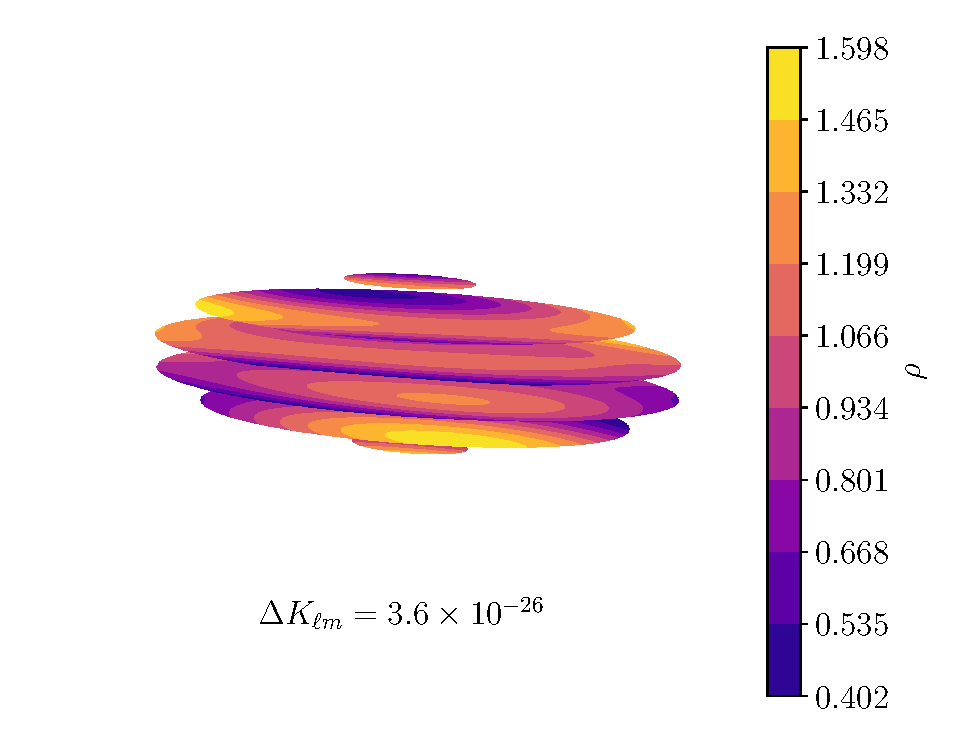
\includegraphics[width=0.33\textwidth]{figs/asym-ell-likelihood.pdf}\hfill
  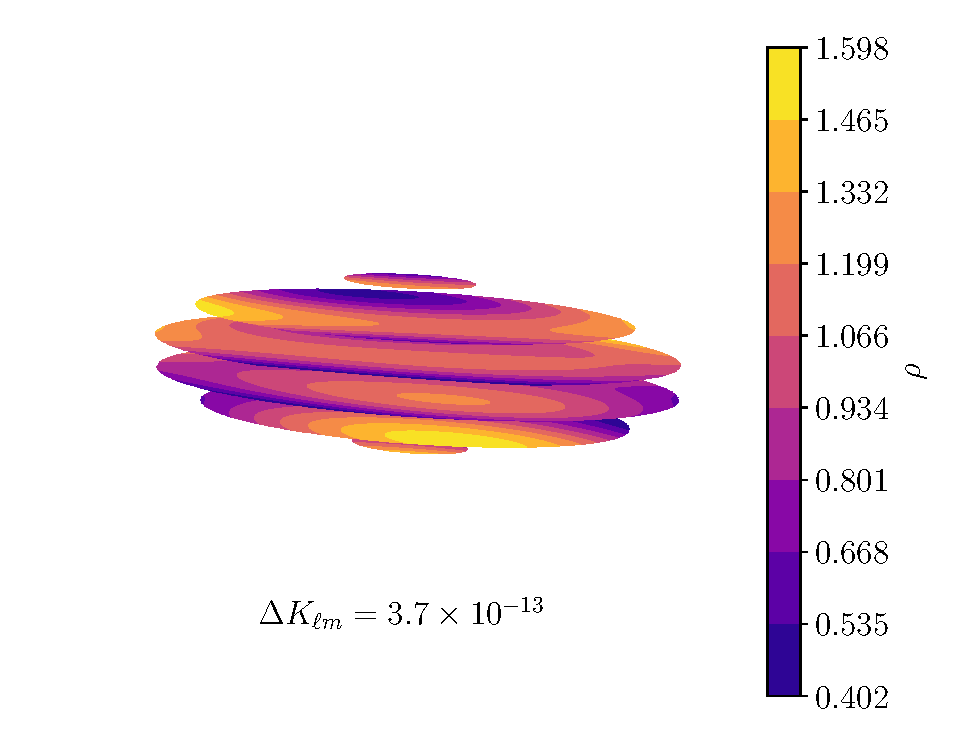
\includegraphics[width=0.33\textwidth]{figs/asym-ell-harmonic.pdf}\hfill
  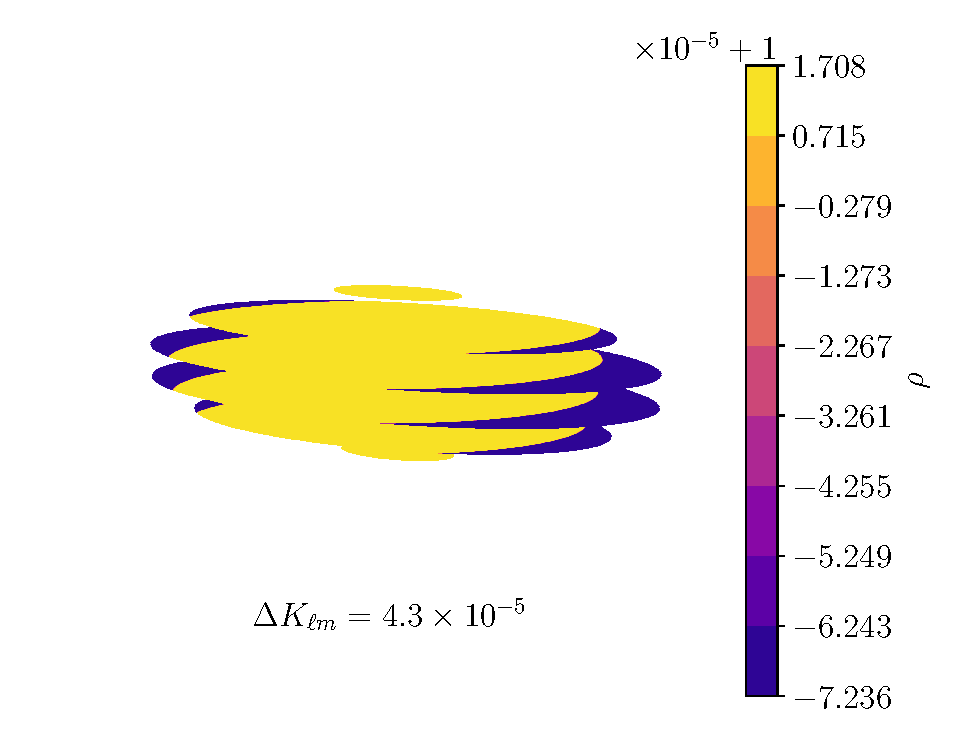
\includegraphics[width=0.33\textwidth]{figs/asym-ell-lumpy.pdf}

  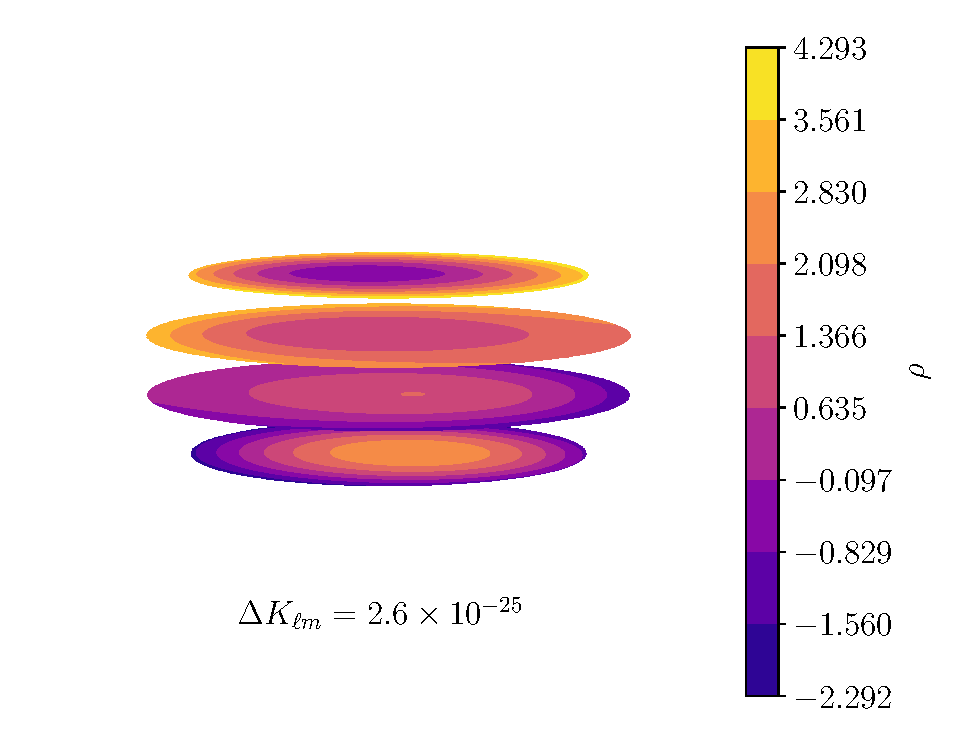
\includegraphics[width=0.33\textwidth]{figs/sym-ell-likelihood.pdf}\hfill
  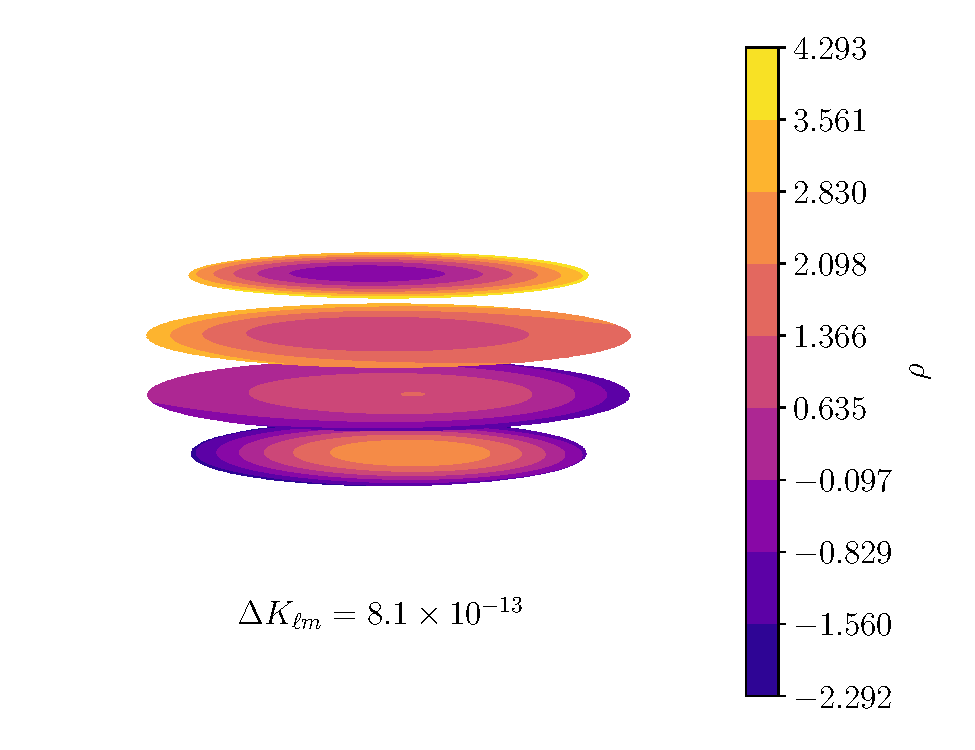
\includegraphics[width=0.33\textwidth]{figs/sym-ell-harmonic.pdf}\hfill
  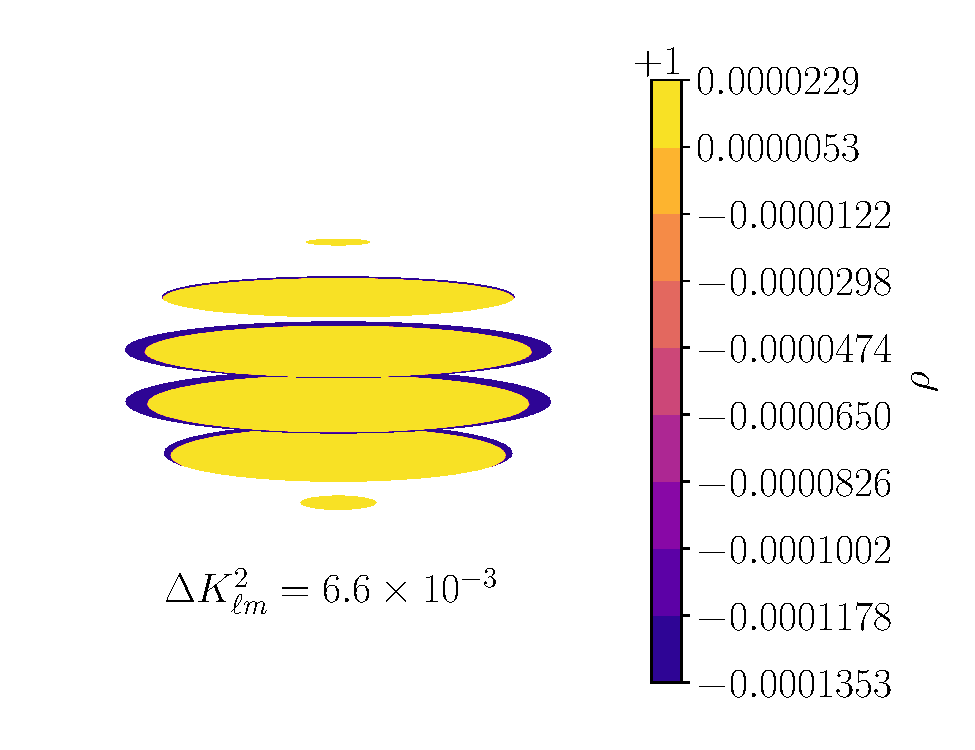
\includegraphics[width=0.33\textwidth]{figs/sym-ell-lumpy.pdf}

  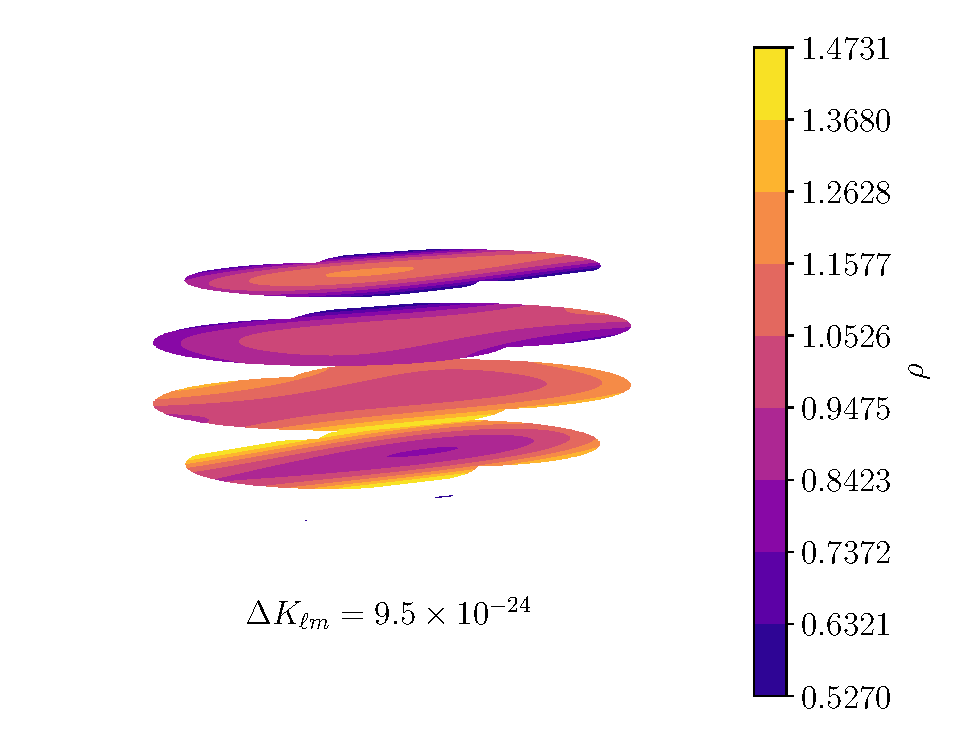
\includegraphics[width=0.33\textwidth]{figs/db-likelihood.pdf}\hfill
  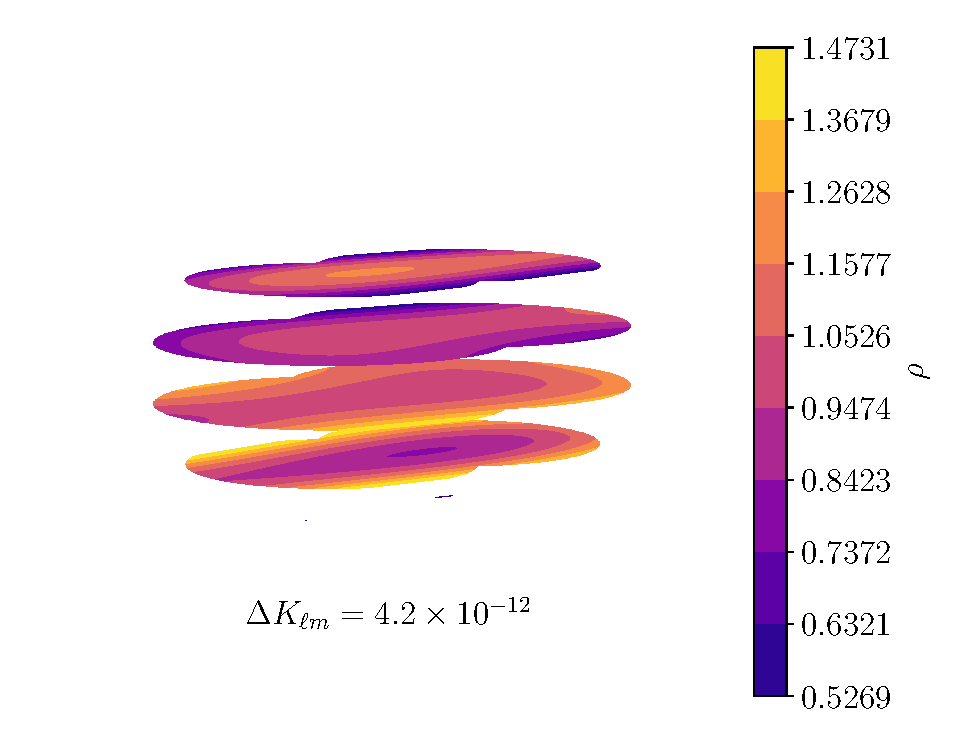
\includegraphics[width=0.33\textwidth]{figs/db-harmonic.pdf}\hfill
  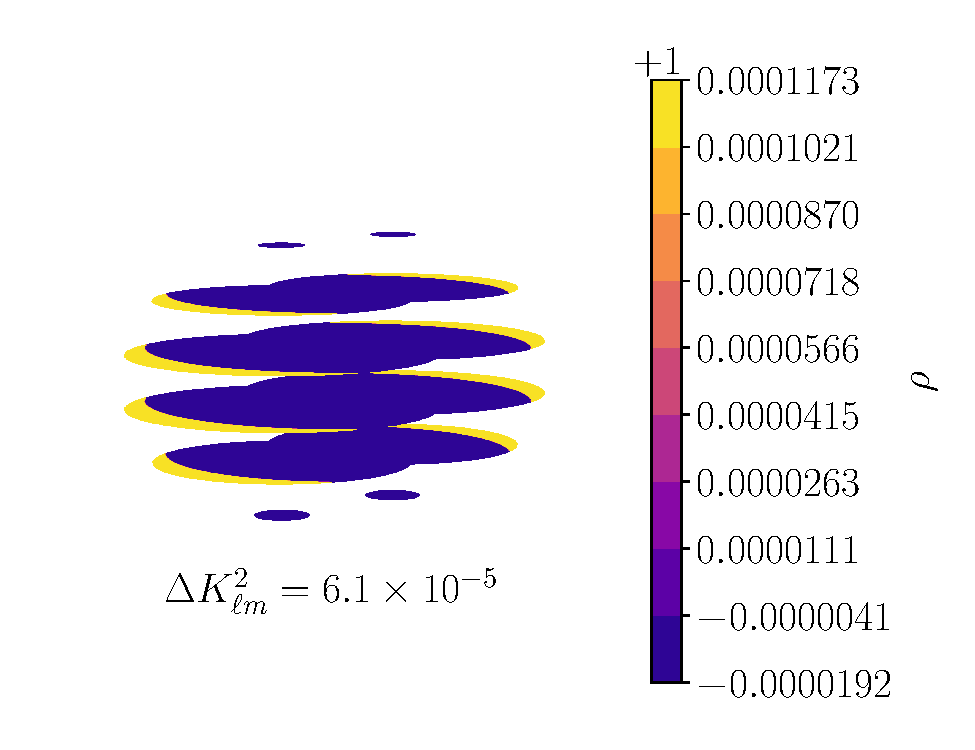
\includegraphics[width=0.33\textwidth]{figs/db-lumpy.pdf}

  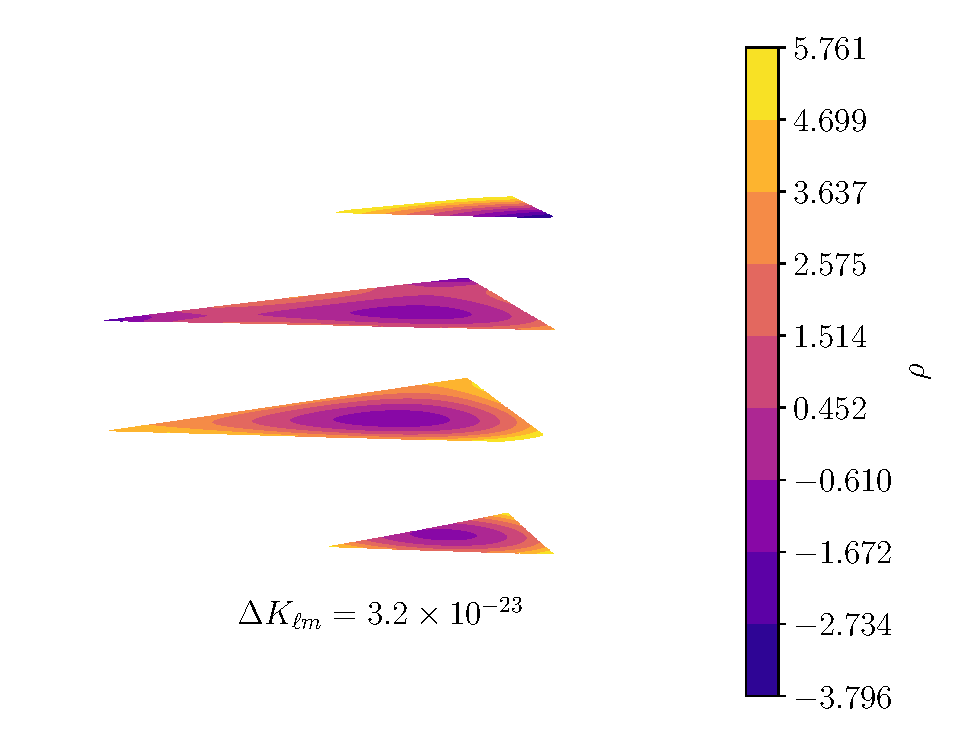
\includegraphics[width=0.33\textwidth]{figs/tet-likelihood.pdf}\hfill
  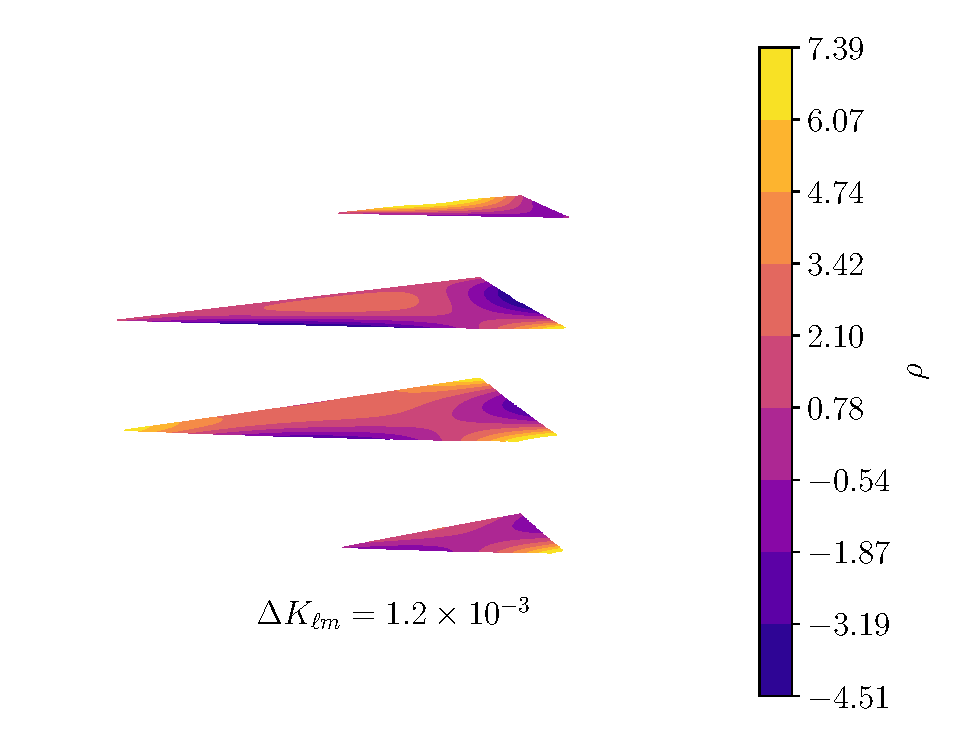
\includegraphics[width=0.33\textwidth]{figs/tet-harmonic.pdf}\hfill
  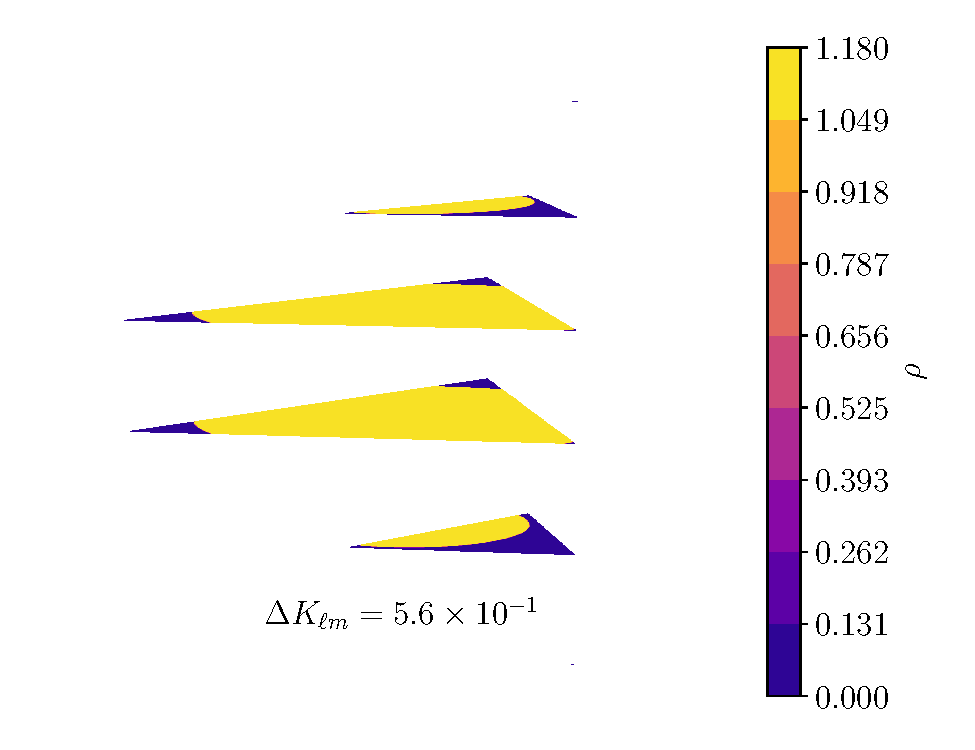
\includegraphics[width=0.33\textwidth]{figs/tet-lumpy.pdf}
  \caption{Density distributions extracted by the likelihood (\textit{left}), harmonic (\textit{middle}), and lumpy with $d=N=1$ (\textit{right}) models from data generated for a uniform-density asteroid. The asteroid shapes are, from top to bottom, the reference asymmetric ellipsoid, the reference symmetric asteroid, the dumbbell model, and a tetrahedron. Density is normalized so that mean density is one. The same distance scale is used in all figures.}
  \label{fig:uniform-density}
\end{figure*}

From figure \ref{fig:uniform-density}, it can be seen that the likelihood and harmonic models produce mostly the same density distributions. This is generally true for uniform density asteroids. This is a useful property because it lends confidence that the models produced are truly representative of the asteorid. The fact that the harmonic model produces very little density moment error ($\Delta K_{\ell m}$) also lends confidence to the distribution; the harmonic model is overdetermined and is not guaranteed to perfectly match the fit-extracted moments.

The asymmetric and dumbbell asteroids produce distributions whose non-uniformity is limited to a factor of 2 or less for the harmonic and likelihood models. This non-uniformity is driven by error in the estimates of the density moments. Note that most of the asteroid does indeed have density close to one in both cases. The lumpy model yields a much more uniform distribution, but only because it is designed to produce uniform lumps. Note that its uncertainty $\Delta K_{\ell m}$ is usually large, both because the model is severely overdetermined (it has 2 degrees of freedom) and because the lump found extends outside the asteroid, violating the assumptions of the model. This is a sign that the lump found does not really exist inside the asteroid.

The symmetric and tetrahedral asteroids are less-well represented. In both cases, the likelihood and harmonic models produce sometimes-negative distributions, and non-uniformity is especially large in the tetrahedral case. This is not the fault of the density models, but rather because both of these asteroids have $K_{22} = 0$ and (as discussed in section \ref{sec:scan-shape}), this leads to degeneracy in $\gamma_0$ and inflated uncertainty in the density moments. In the tetrahedral case, the problem is worsened because $K_{20}=0$ as well, so that torque is dominated by the small and ill-constrained $K_{3m}$ components.

Uncertainty in each distribution was calculated but not shown. The size of uncertainty is such that the density distribution is largely consistent with uniform at all points for all models(within 1-2$\sigma$), with a small fraction of low-uncertainty regions which are inconsistent with uniform. Uncertainty is generally larger towards the edges of the distribution, both for these shapes and for the shapes shown in the following sections.

From these examples, we may draw the conclusions that all three models produce density distributions generally consistent with uniform for uniform asteroids. The most likely distributions are themselves mostly uniform, but can still produce non-uniformities as large as a factor of 2 in certain regions due to uncertainty in $K_{\ell m}$. Asymmetric asteroids such as the dumbbell and the asymmetric reference asteroids yield the best results because they have $K_{22} \neq 0$ and therefore do not suffer from degeneracy in initial orientation. Finally, the lumpy model can generally be ruled out in these cases because it produces nonphysical results.

\subsubsection{Spherical shape test}
We test the sensitivity of the density distributions to incorrect estimates for the shape of the asteroid by obtaining density moments from an ellipsoidal asteroid encounter and attempting to extract density distributions assuming a spherical shape. We do this for the asymmetric and symmetric reference asteroids, with density distributions shown in figure \ref{fig:sphere-density}.

\begin{figure*}
  \centering
  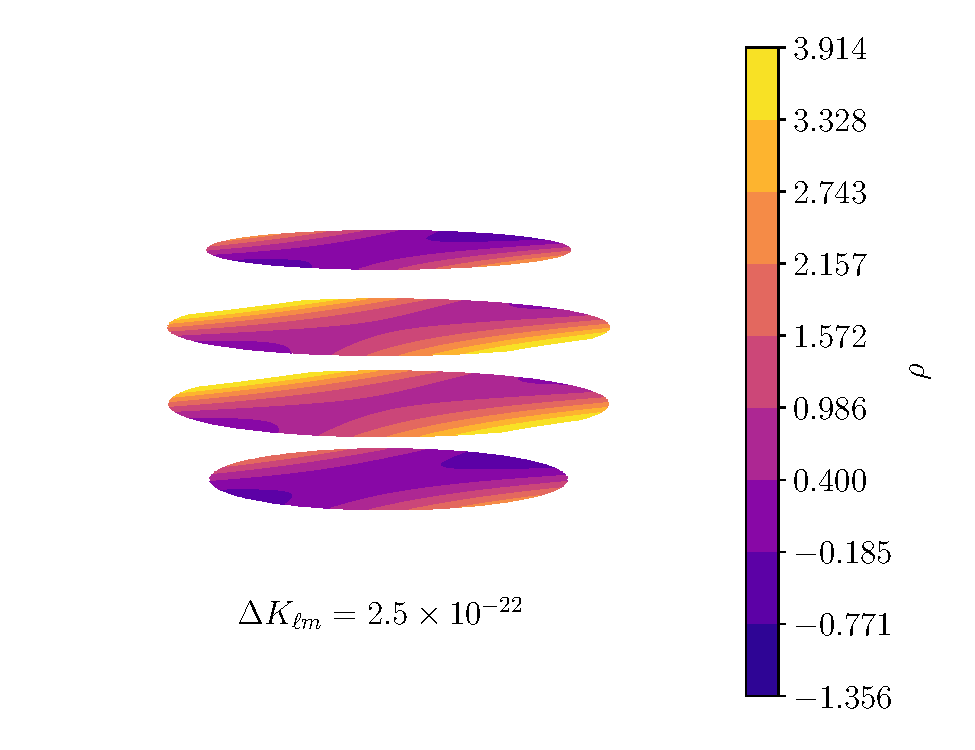
\includegraphics[width=0.33\textwidth]{figs/asym-sph-likelihood.pdf}\hfill
  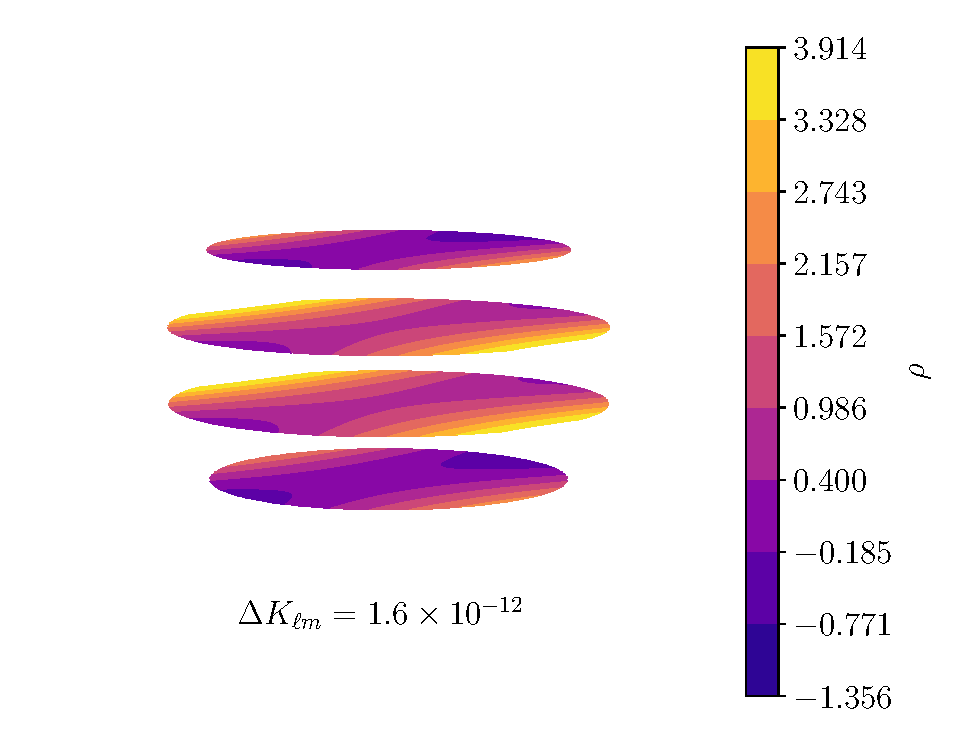
\includegraphics[width=0.33\textwidth]{figs/asym-sph-harmonic.pdf}\hfill
  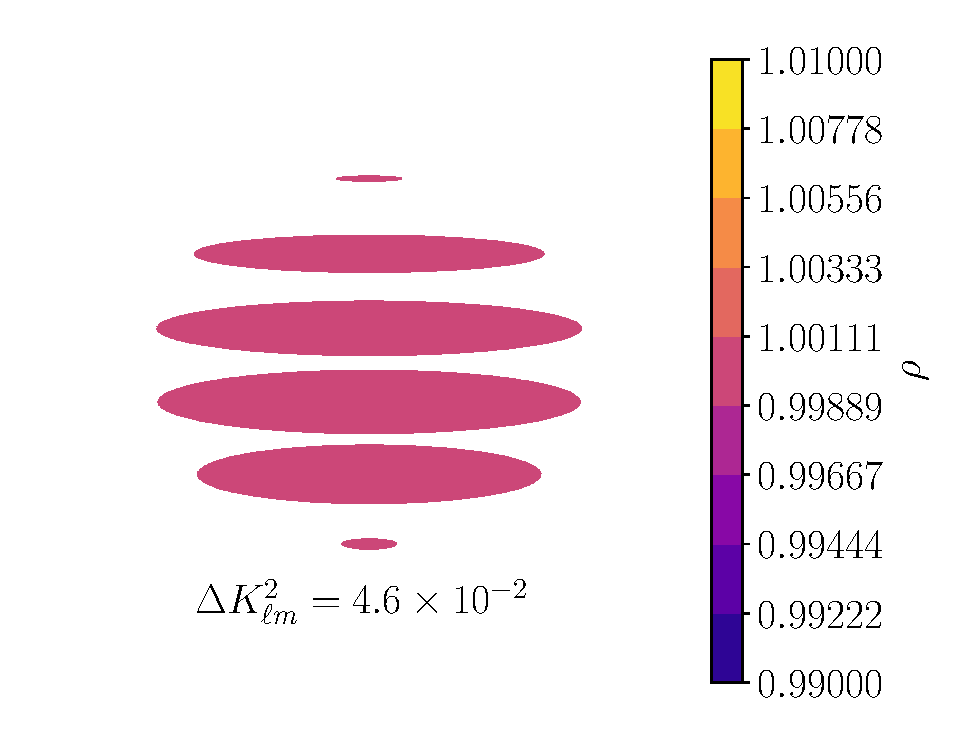
\includegraphics[width=0.33\textwidth]{figs/asym-sph-lumpy.pdf}

  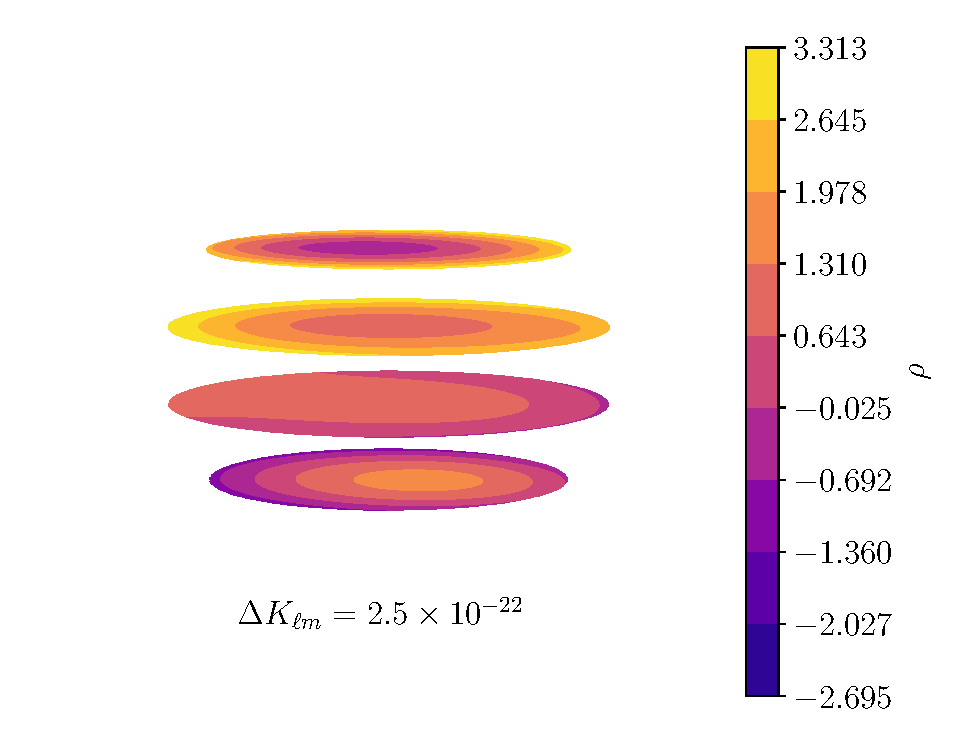
\includegraphics[width=0.33\textwidth]{figs/sym-sph-likelihood.pdf}\hfill
  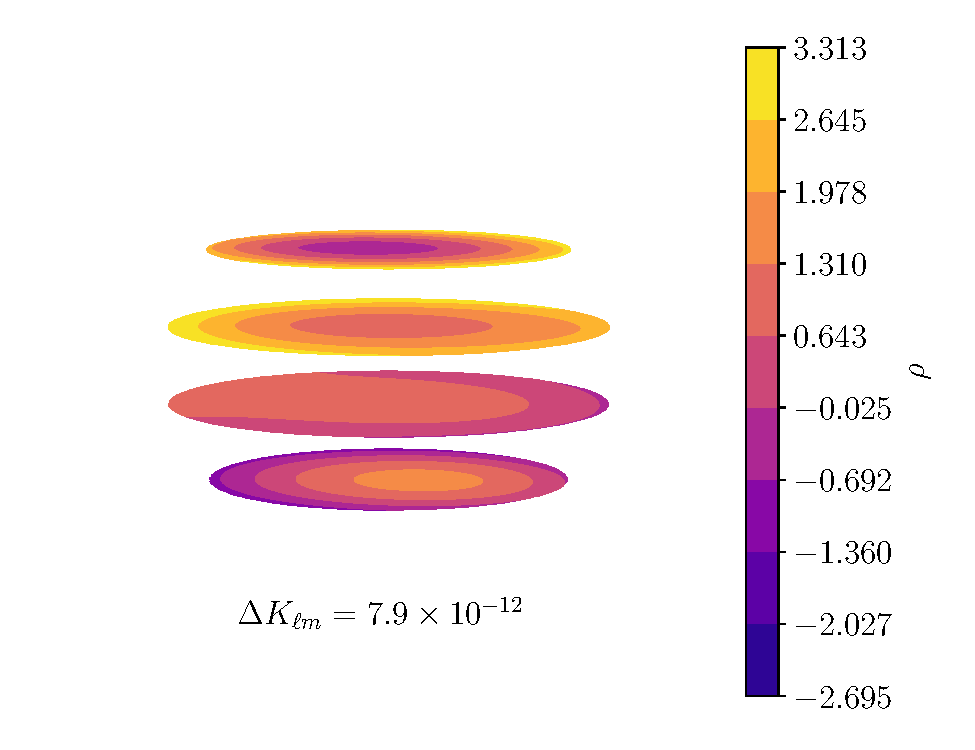
\includegraphics[width=0.33\textwidth]{figs/sym-sph-harmonic.pdf}\hfill
  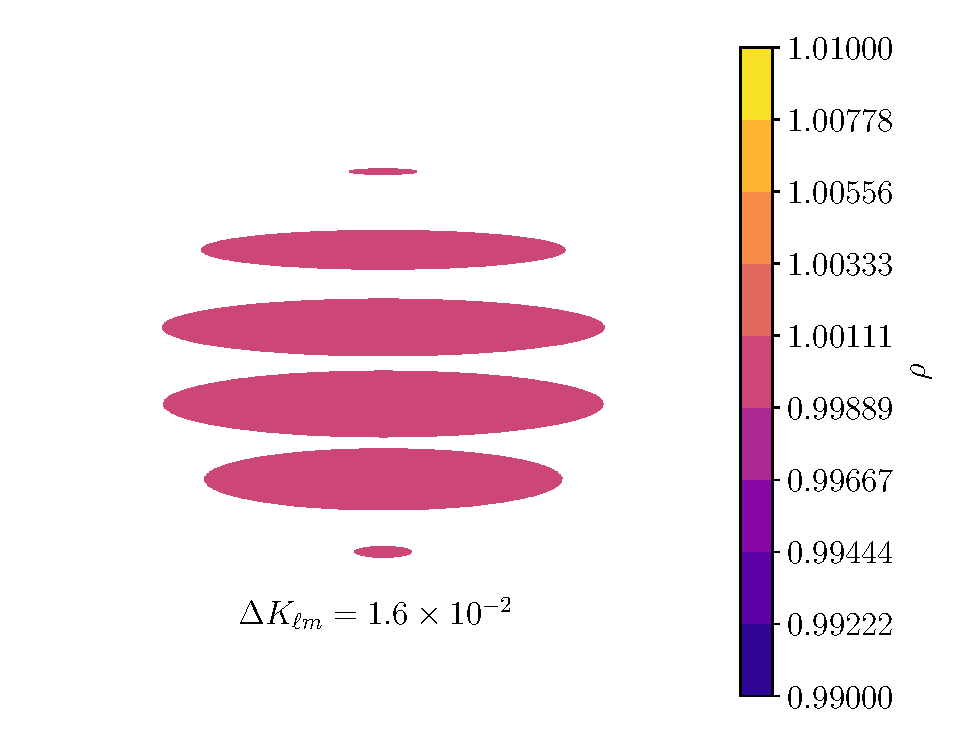
\includegraphics[width=0.33\textwidth]{figs/sym-sph-lumpy.pdf}\

  \caption{Density distributions extracted by the likelihood (\textit{left}), harmonic (\textit{middle}), and lumpy with $d=N=1$ (\textit{right}) models from data generated for a uniform-density asteroid. The original asteroid shapes were the reference asymmetric (\textit{top}) and symmetric (\textit{bottom}) ellipsoids. In both cases, the density distributions have been extracted assuming a spherical shape. Density is normalized so that mean density is one. The same distance scale is used in all figures.}
  \label{fig:sphere-density}
\end{figure*}

Both the likelihood and harmonic models are accurate in that $\Delta K_{\ell m}$ is low, and they produce similar distributions as in the previous section. Before, we took this fact as a signal that the distributions are likely to be correct. However, now they both produce negative density distributions for both asteroid shapes. This is a signal that the shape model is incorrect, and indeed the density distribution allows us to determine exactly how the shape model is wrong. In the asymmetric ellipsoid case, the density distribution is small (even negative) at large $|z|$ (up in the figure). The density is large at large $|y|$ (front right in the figure). Comparison with the asymmetric reference asteroid depicted in figure \ref{fig:uniform-density} shows that the low-density region is outside the true asteroid shape, and the high-density region is inside. In other words, the shape can be corrected by extending it where density is large and retracting it where density is low.

A similar statement is true for the symmetric ellipsoid case in that density is low near the poles, but this time the regions with large density are evenly distributed around the equator, indicating the symmetry of the original asteroid.

The lumpy model produces lumps so large that they dominate the asteroid, predicting uniform distribution with $K_{\ell m} = 0$ for $\ell \geq 1$.. The error in density moments $\Delta K_{\ell m}$ is therefore very large, equal to the sum of $|K_{\ell m}|$ for the original asteroids.

In short, severely incorrect shape estimates can be caught for all three models by negative predicted densities or by the failure of the density distribution model to match the extracted density moments. The shape can be corrected by extending it where the density distribution is high and retracting it where the density distribution is low.


\subsubsection{Nonuniformity test}
\label{sec:non-uniform-density}

We also test several non-uniform density asteroids and compare the generated density distributions for all three models to see if the non-uniformities are recovered. We consider two asteroids, one with mass concentrated in the middle, and one with mass concentrated around the edges. (Specifically, the mass distribution follows a spherically symmetric exponential $\rho(r) \propto e^{\pm r^2/a_m^2}$). To prevent the problems seen in previous sections when a symmetric asteroid is simulated, we set the shape of the asteroids to the asymmetric reference asteroid. The extracted density distributions are shown in figure \ref{fig:non-uniform-density}

\begin{figure*}
  \centering
  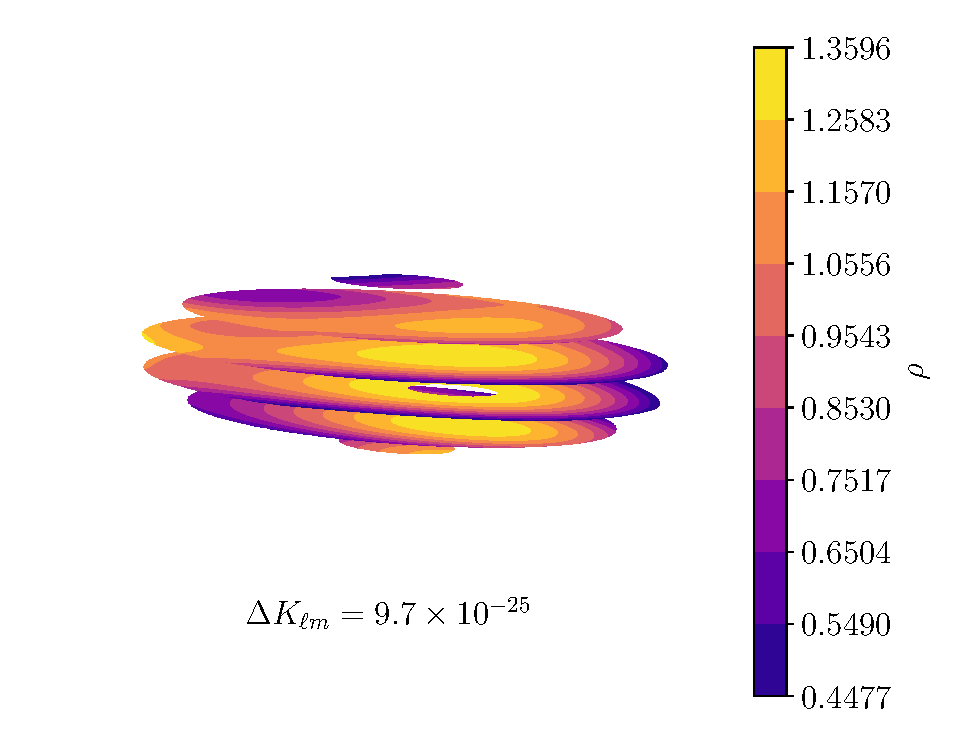
\includegraphics[width=0.33\textwidth]{figs/in-likelihood.pdf}\hfill
  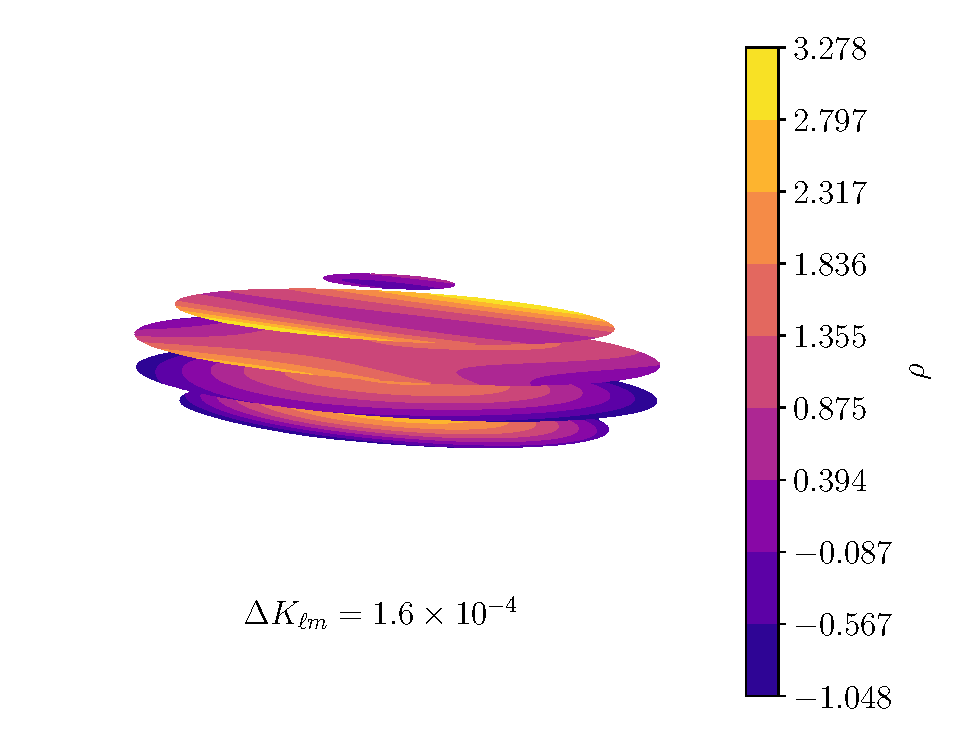
\includegraphics[width=0.33\textwidth]{figs/in-harmonic.pdf}\hfill
  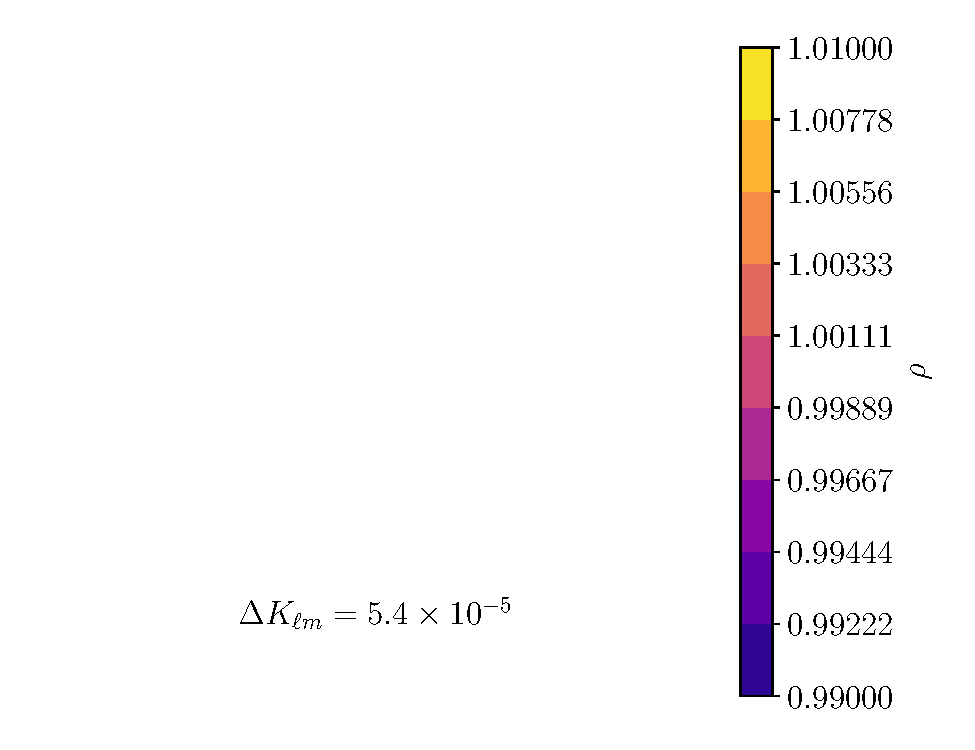
\includegraphics[width=0.33\textwidth]{figs/in-lumpy.pdf}

  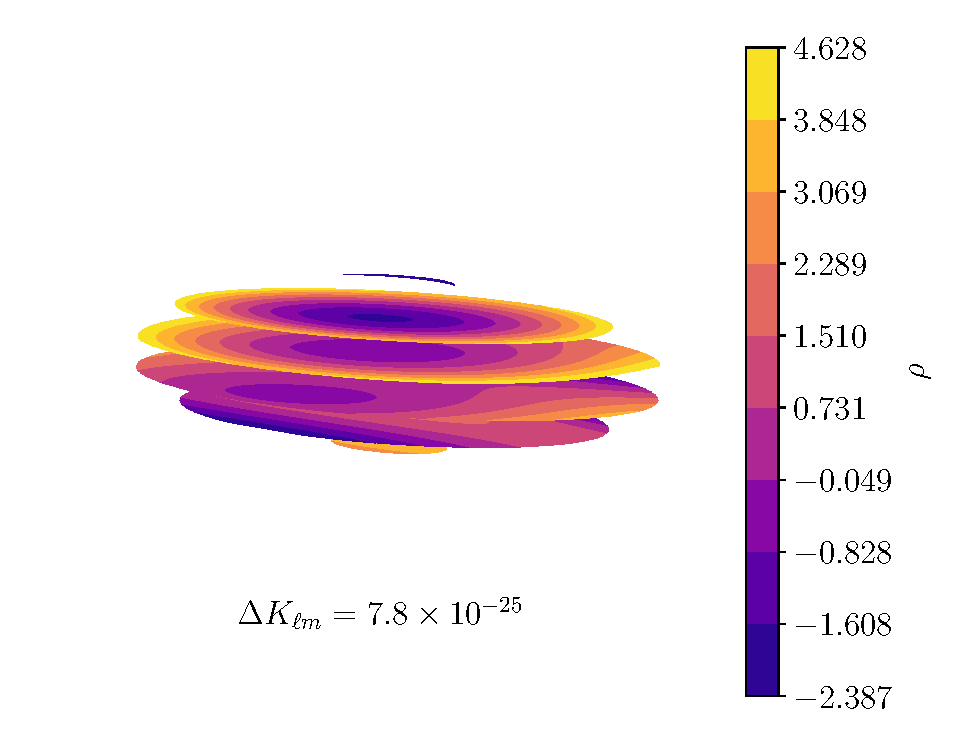
\includegraphics[width=0.33\textwidth]{figs/out-likelihood.pdf}\hfill
  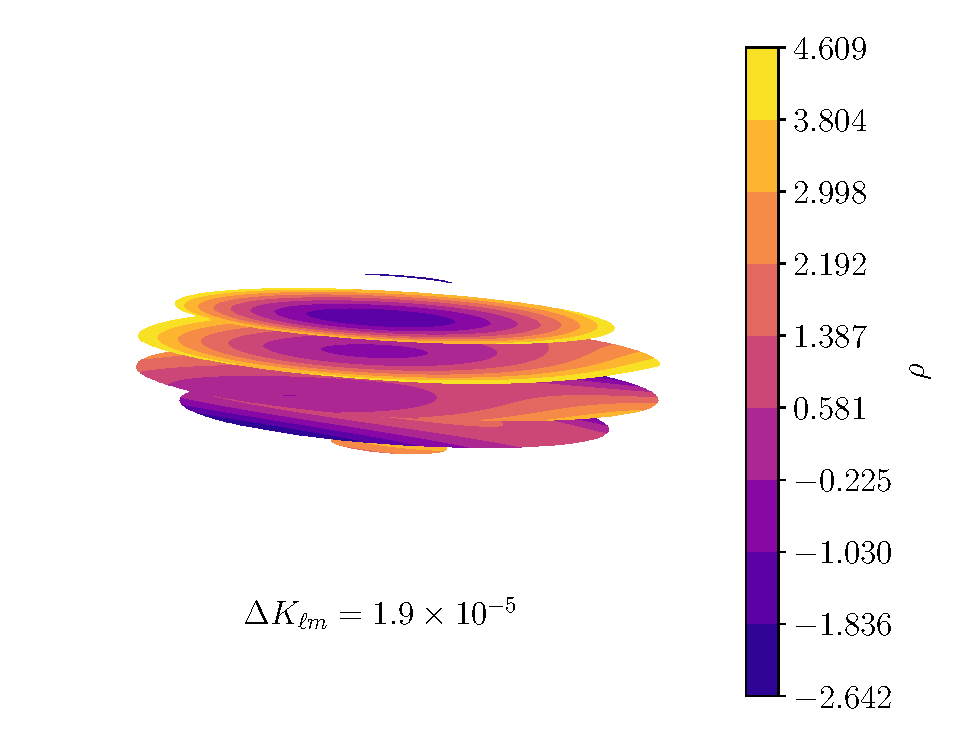
\includegraphics[width=0.33\textwidth]{figs/out-harmonic.pdf}\hfill
  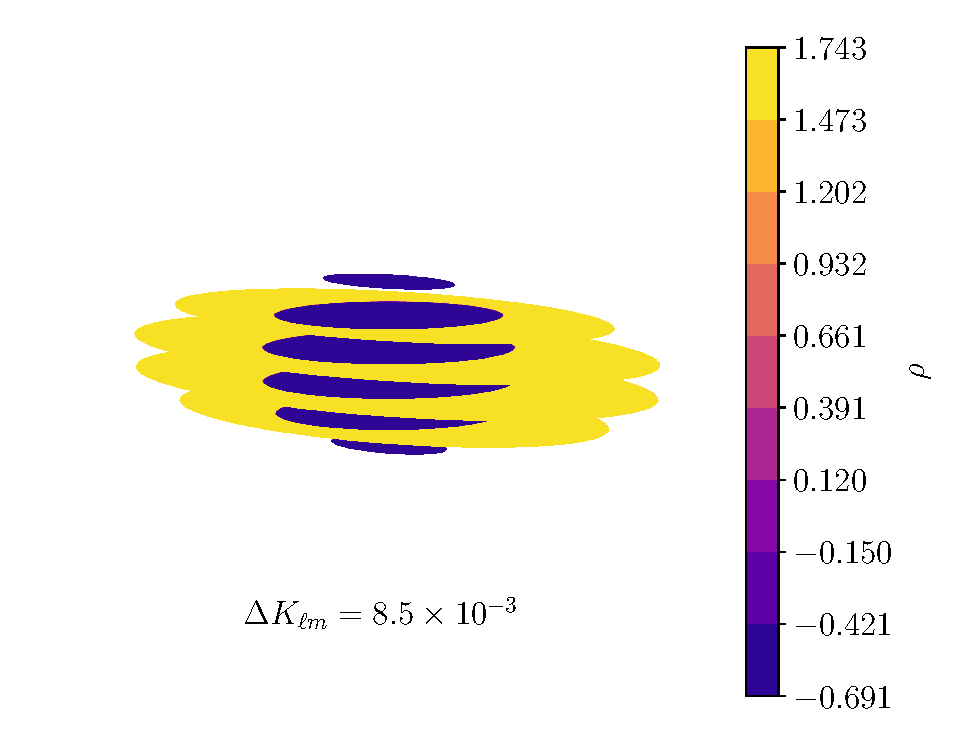
\includegraphics[width=0.33\textwidth]{figs/out-lumpy.pdf}\

  \caption{Density distributions extracted by the likelihood (\textit{left}), harmonic (\textit{middle}), and lumpy with $d=N=1$ (\textit{right}) models from data generated for non-uniform-density asteroids with mass concentrated in the middle (\textit{top}) and the edges (\textit{bottom}).Density is normalized so that mean density is one. The same distance scale is used in all figures.}
  \label{fig:non-uniform-density}
\end{figure*}

For these non-uniform asteroids, the likelihood and harmonic model do not coincide, as can be seen by comparing the density distributions and the fact that $\Delta K_{\ell m}$ is much larger for the harmonic distribution (indicating that the true density distribution is not harmonic). However, the two models do give similar results. Comparing the center-weighted asteroid and the edge-weighted asteroid distributions, one can see that the center-weighted case indeed places more mass in the center of the asteroid shape for the harmonic and likelihood models, while the edge-weighted asteroid places mass at the edges.

Though the general mass placement arrived at by both the likelihood and harmonic models is accurate, the precise density distributions are inaccurate because they predict negative densities. This might be addressed for the likelihood model by selecting a likelihood that strongly disfavors negative densities, such as a log-normal distribution. However, this would sacrifice the linearity of the model, so we do not do so here, accepting the fact that for strongly varying distributions, the harmonic and likelihood models may predict negative density distributions.

Figure \ref{fig:non-uniform-density} shows that the lumpy model places one large lump of greater density than the surrounding medium for the center-weighted asteroid and less density for the edge-weighted asteroid, as expected. Greater error is incurred in $\Delta K_{\ell m}$ in this lumpy model than for the harmonic and likelihood models due to the lumpy model's crudeness, but the lump gives a qualitative estimate of the density distribution of the asteroid which is useful for interpreting the other two models. Note that the lumpy model predicts negative density in the the edge-weighted scenario like the other two models.


The lumpy model has one caveat that has not yet been illustrated, which applies for $N=d=1$ if (1) the center of mass of the asteroid is the centroid of the asteroid shape and (2) the density moments of the asteroid shape assuming uniform density are proportional to the fitted density moments. (1) guarantees that the lump will be placed at the origin and therefore will not contribute to $K_{\ell m}$ for $\ell \geq 1$, and (2) guarantees that the mass of the asteroid shape will be chosen such that the shape density moments exactly match the fitted density moments. The lump radius will then be set to zero because the fitted density moments are already matched. This zero-radius-lump result will occur even if the true density distribution has a large-radius lump at the origin.

An example of this caveat applied is an elliptical lump inside a similar elliptical asteroid. This is why, in the center-weighted and edge-weighted density distributions, we specifically chose a spherically symmetric density distribution for our ellipsoidal asteroid shape, rather than an ellipsoidal distribution. Thus, the caveat is avoided.



\subsubsection{Lump test}

Finally, we test an asteroid with a discrete change in density distribution (for example, a boulder), of the kind that the lumpy model is designed to detect. We place a spherical mass of density six times the density of the surrounding medium inside the asymmetric reference asteroid, slightly displaced along $\unit y$. The rest of the asteroid we set to uniform density. The density distributions found by the three model for this asteroid are shown in figure \ref{fig:blob-density}.

\begin{figure*}
  \centering
  \includegraphics[width=0.33\textwidth]{figs/blob-likelihood.pdf}\hfill
  \includegraphics[width=0.33\textwidth]{figs/blob-harmonic.pdf}\hfill
  \includegraphics[width=0.33\textwidth]{figs/blob-lumpy.pdf}

  \caption{Density distributions extracted by the likelihood (\textit{left}), harmonic (\textit{middle}), and lumpy with $d=N=1$ (\textit{right}) models from data generated for an asteroid with an off-center lump. Density is normalized so that mean density is one. The same distance scale is used in all figures.}
  \label{fig:blob-density}
\end{figure*}

We see from figure \ref{fig:blob-density} that the harmonic and likelihood model fail completely to recover the presence or location of the lump. There appears to be a slight increase of density in roughly the correct location for both models, but this is not a statistically significant effect, and can be seen in other asteroid such as the center-weighted asteroid of figure \ref{fig:non-uniform-density}. Also like figure \ref{fig:non-uniform-density}, we see that the harmonic and likelihood models do not agree exactly, and the failure of the harmonic model to exactly reproduce $K_{\ell m}$ suggests that the true distribution is not harmonic.

The failure of these models to find lumps is expected, since $K_{\ell m}$ is most sensitive to non-uniformities of characteristic size $\pi/(\ell + 1)$ radians in the polar direction, and $2\pi / (|m|+1)$ in the azimuthal direction by the definition of $Y_{\ell m}$. This lump is too small to be resolvable by $K_{3m}$, so we do not expect most models to find it.

However, the lumpy model computes the location and density of the mass very well. Some inaccuracies are induced by the uncertainty in $K_{3m}$, which changes the minimum of equation \ref{lump-minimize} such that the lump is displaced by 9 m along $\unit y$ from where it should be. This in turn causes a 70 m inaccuracy in the lump's radius. Nevertheless, the accuracy is still very good compared to other models, and we conclude that the lumpy model is capable of recreating the location of lumps (except for the caveat mentioned in the previous section for distributions with $K_{\ell m}$ proportional to the asteroid shape's moments). But the ability of the lumpy model to place a lump does not guarantee the lump to actually exist, as was seen in all the other asteroid distributions analyzed here.

\section{Conclusions}

We assess the feasibility of extracting density moments and density distributions for a general asteroid encounters, and ask what encounter properties are necessary to obtain the most information about asteroid density.

We derived a novel, arbitrary-order equation for the tidal torque experienced by an asteroid during an encounter with a planet of arbitrary shape and mass distribution. The tidal torque (equation \ref{eqn:tidal-torque}) is a function only of the density moments of the asteroid $K_{\ell m}$, the asteroid orbit, and the initial asteroid orientation. This equation revealed that the rotational velocity of the asteroid over time depends strongly on $K_{\ell m}$ and the initial orientation.

We built a fast simulation for an asteroid flyby, truncating the equation at second order, and used the simulation to extract first- and second-order density moments from synthetic spin pole data via a Markov Chain Monte Carlo fit. Other studies have extracted the first-order moments from encounters, but not second order. We observe the following general properties of the moments:
\begin{enumerate}
  \item The second-order moments $K_{3m}$ are generally a factor of $~\frac{a_m}{r_p}$ more uncertain than the first-order moments, where $a_m$ is the asteroid radius and $r_p$ is the perigee distance. For our reference asteroid, this fraction was about $10^{-5}$.
  \item Of the seven second-order moments, those that measure small-scale variations in density (i.e., $|m|$ is large) are generally less uncertain.
  \item The oblateness of the central body cannot be ignored without generating incorrect density moment estimates, but a nonzero oblateness does not greatly increase the precision of the extracted moments except perhaps when a moon is present.
\end{enumerate}

We assessed the posterior uncertainty generated by the fit process by adjusting eleven parameters of an asteroid on an Earth flyby. The main conclusions are listed below.

\begin{enumerate}
  \item Highly precise rotational velocity data is required to produce precise  moments. Especially the uncertainty on the asteroid rotational period must be small compared to the uncertainty on asteroid spin pole. Our reference asteroid, with $\sigma P/P = 10^{-5}$ and the spin pole known to within a few degrees of error, was accurate enough.
  \item A close encounter is vital for accurate second-order moment extraction, though some of the second-order moments can still be required for more distant encounters, extending to about a third of a Lunar distance for the reference asteroid.
  \item The asteroid rotational period must not be too small (smaller than about 5 hours, although $K_{30}$ will become unresolved at for periods smaller than 8 hours). Nor must the asteroid's rotational velocity point in an inconvenient direction (orthogonal to the orbital plane, or in the orbital plane and perpendicular to the perigee vector).
  \item The cadence of observation should be shorted than about 30 minutes (except $K_{30}$ will become unresolved for cadence worse than 10 minutes). Gaps of data can appear, specifically at perigee, but only for a little over an hour given 2 minute cadence before the posterior uncertainty significantly increases.
\end{enumerate}

Finally, we present three fast, linear methods for extracting density distributions (together with uncertainties) from the density moments and the shape of the asteroid as obtained by light-curve analysis. The extracted density distributions largely are consistent with the true distributions in all cases we tested. Slight errors in $K_{3m}$ dramatically change the overall distribution, so that they are not very precise. Indeed, the models sometimes predict negative density (though more complicated models could be made not to). Errors in the shape estimate of teh asteroid also distort the density distribution. Nevertheless, large-scale properties of the asteroid's true distribution, such as whether the mass is located in the middle or on the edges, are often observable. Two of the models presented (the harmonic and lumpy models) are flexible in their number of parameters, so that if only these large-scale properties are necessary, a small set of parameters can be chosen to prevent over-fitting.

In the appendices, we answer more specific questions about the behavior of the tidal torque system and the fit process that might arise.

\section*{Acknowledgements}

We warmly thank Emmanuel Jehin, Maxime Devogele, and Marin \jtd{What's Marin's last name?} for meeting with the authors to discuss this work, and pointing out possible future directions to take it. JTD would like to thank the Massachusetts Institute of Technology Undergraduate Research Opportunities Program (MIT UROP) office for funding his work for many semesters, and their flexibility in funding students from departments other than the source of funding. The work of JdW was funded by \jtd{Who funds Julien?}. Much of the computation shown in this paper was executed on MIT Supercloud's facilities.



%%%%%%%%%%%%%%%%%%%%%%%%%%%%%%%%%%%%%%%%%%%%%%%%%%
\section*{Data Availability}

The code used to generate data, fit density moments to it, and extract density distributions from the moments is available on \href{https://github.com/jack-dinsmore/asteroid-tidal-torque}{GitHub}, or by contacting JTD.



%%%%%%%%%%%%%%%%%%%% REFERENCES %%%%%%%%%%%%%%%%%%

\bibliographystyle{mnras}
\bibliography{asteroids.bib}

%%%%%%%%%%%%%%%%%%%%%%%%%%%%%%%%%%%%%%%%%%%%%%%%%%

%%%%%%%%%%%%%%%%% APPENDICES %%%%%%%%%%%%%%%%%%%%%

\appendix

\section{Reference asteroid configurations}
\label{app:reference-configs}

Except when otherwise mentioned, we use the following asteroid encounter parameters. Many of the parameter choices are made to maximize the quality of observations (a close orbit, large asteroid, etc.) This is so that our uncertainties have room to grow; if the reference asteroid has low uncertainty,

\begin{enumerate}
  \item An orbit around Earth with $6$ km s$^{-1}$ excess velocity and perigee at 5 Earth radii. This orbit was chosen to roughly match that of 99942 Apophis \cite{giorgini2005recent, smalley20052004}. These orbital parameters correspond to an eccentricity of 3.88.
  \item An initial roll of $\gamma_0=\pi/8$.
  \item A cadence of 2 minutes and observational uncertainty of $\sigma_\theta = 0.01$ and $\sigma_\rho / \sigma_\theta = 10^{-5}$.
  \item A rotational period of 9 hours, with the rotational velocity vector distributed between the $\unit X$, $\unit Y$, and $\unit Z$ axes in a $1:2:-2$ ratio.
  \item An asteroid with radius $a_m = 1$ km and $K_{3m}=0$. For $K_{22}$ and $K_{20}$, we use two standard values. One with $(K_{22}, K_{20}) = (0, -0.097)$ and one with $(0.052, -0.202)$. Including the third point obtained by reflection $K_{22}\rightarrow -K_{22}$, these are the three points that minimize the mean distance between an arbitrary point in the allowed parameter space (equation \ref{eqn:parameter-bounds}) and these reference values. The first point is called the symmetric case because the corresponding uniform-density-ellipsoid model is rotationally symmetric around $\unit z$. The second case and its reflection are called the asymmetric cases. Values of $(0.052, -0.202)$ have $a < b$ in the ellipsoid model, and the reflected value has $a > b$. If not specified, we use the $a < b$ case. Specifically, the asymmetric case has $a=1140$ m, $b=1839$ m, and $c=565$ m, while the symmetric case has $a=b=1411$ m and $c=1008$ m.
\end{enumerate}

We use the asymmetric ellipsoid in nearly all runs, do to the degeneracy induced in our model when $K_{22} = 0$.


\section{The cadence cutoff}
\label{app:cadence-tests}

In section \ref{sec:scan-cadence}, we noted that posterior uncertainty as a function of observation cadence $\Delta t$ appears to increase suddenly near $\Delta t \sim T_\text{cad}=30-40$ min. We mentioned that this cadence cutoff is likely a function both of the rotational period of the asteroid and the time spent near perigee. We study this cutoff in closer detal in this appendix.

We measure the dependence of the cadence cutoff on rotational period by varying the period $P_\omega$ and reproducing figure \ref{fig:scan-cadence}; i.e., we run many simulations of the changed $P_\omega$ with different cadences and plot the posterior fit uncertainty $\sigma$ as a function of cadence $\Delta t$. Specifically, we use $P_\omega = 5$ hr and 20 hr, roughly double and half of the reference 9 hr. The resulting curves of $\sigma(\Delta t)$ are shown in figure \ref{fig:cad-period}, with each normalized so that their maximum values is 1 so that changes to $\sigma$ induced by the change in $P_\omega$ that are not a function of $\Delta t$ and therefore irrelevant here (i.e., those studied in section \ref{sec:scan-period}), are removed.

\begin{figure}
  \centering
  \includegraphics[height=0.89\textheight]{figs/cad-period.pdf}
  \caption{1-$\sigma$ confidence intervals plotted as a function of cadence $\Delta t$ for periods of 9 hr (the reference asteroid, solid colored lines), and 5 hours (dotted lines), and 20 hours (dashed lines). Confidence intervals have been normalized for the sake of comparison, so that the maximum for each curve is 1.}
  \label{fig:cad-period}
\end{figure}

We also wish to capture dependence on the time spent by the asteroid near perigee, but we do not wish to change the orbit shape or central body, because this may induce other effects that could also affect the cadence plot. Instead, we adjust the speed at which the asteroid moves through the orbit. In one instance, the asteroid's path is artificially slowed by a factor of 2, which we denote as $t_\text{spin}/t_\text{orbit}=0.5$; in the other instance, $t_\text{spin}/t_\text{orbit}=2$, meaning that the orbit is sped up. This approach of changing the speed of the orbit is meant to approximate changes to $T_p$ defined in equation \ref{eqn:tp}. The posterior uncertainties for these two cases and the original case are shown in figure \ref{fig:cad-speed}. Again, $\sigma$ is normalized so that $\Delta t$-independent variations are removed. However, the $t_\text{spin}/t_\text{orbit}=2$ uncertainties begin to fill the prior distribution for large $\Delta t$ for some parameters, which can be seen by discontinuous variation in the dotted line of figure \ref{fig:cad-speed}.

\begin{figure}
  \centering
  \includegraphics[height=0.89\textheight]{figs/cad-speed.pdf}
  \caption{1-$\sigma$ confidence intervals plotted as a function of the orbit time scaling $t_\text{spin}/t_\text{orbit}$ for no scaling (the reference asteroid, solid colored lines), time doubling (dotted lines), and halving (dashed lines). See text for the definition of $t_\text{spin}/t_\text{orbit}$. Confidence intervals have been normalized for the sake of comparison, so that the maximum for each curve is 1.}
  \label{fig:cad-speed}
\end{figure}

Many of the curves in figures \ref{fig:cad-period} and \ref{fig:cad-speed} show a cadence cutoff at $T_\text{cad} \sim 30-60$ min. Those that show no cutoff (i.e., they merely smoothly increase over $\Delta t$) may in fact exhibit a cutoff $T_\text{cad} > 60$ min, which is off the plot. By comparing $\sigma(\Delta t)$ for a specific parameter, we see that the dotted lines often (but not always) reach the cadence cutoff before the solid line. For example, in figure \ref{fig:cad-period}, this effect is especially clear for $K_{22}$, $K_{33}$, $\Im K_{22}$, and $\Re K_{31}$, but the opposite appears for $\Re K_{32}$. The dotted curves are significant in both figures because they represent smaller $\sigma$ cases. Section \ref{sec:scan-period} reveals that long-rotational-period asteroids lead to smaller $\sigma$, and $t_\text{spin}/t_\text{orbit} < 1$ leads to smaller $\sigma$ because of the presence of more perigee data. It therefore appears that large $P_\omega$ and large times spent at perigee move the cadence cutoff to larger $\Delta t$.

The dependence of the exact location of the cadence cutoff is likely more complicated than the above analysis indicates. However, large uncertainties induced by small $P_\omega$ or large $t_\text{spin}/t_\text{orbit}$ makes it difficult to produce data which are not affected by the finite size of the prior (as figure \ref{fig:scan-speed} was) to study these regimes. Computation time and random variation in $\sigma$ also limits us. We therefore do not attempt to explore the dependence between $T_\text{cad}$ and the encounter parameters further. If a future analysis does require a detailed understanding of how cadence affects uncertainty for a specific encounter, our simulation and fit process can be run given the parameters of the encounter in question in a similar manner to section \ref{sec:scan-cadence}. 


\section{Comparison of Jupiter and Earth flyby}
\label{app:jupiter-earth}

If sufficiently accurate spin pole data can be detected for non-Earth encounters, it may be possible to extract density moments for encounters with larger planets. In this appendix, we run our reference asteroid through a Jupiter encounter to analyze the differences in uncertainty.

The physical parameters of the asteroid body are kept the same as the Earth encounter case (listed in appendix \ref{app:reference-configs}), as are the observational uncertainty and cadence. The orbit is adjusted for the Jupiter case by setting a perijove distance of $r_p=5$ Jupiter radii (compared to perigee radius $r_p=5$ Earth radii for the Earth encounter). We perform two fits for two different values of $v_\infty$: in one case we keep the Earth-encounter value of $v_\infty = 6$ km s$^{-1}$, and in the other case we increase the velocity such that the eccentricity (and therefore the angle between the orbits' hyperbolic asymptotes) are the same for both encounters. The latter requires $v_\infty = \sqrt{G\mu_M/r_p (e-1)}=32$ km s$^{-1}$. The rationale for these excess velocity values is that, for $v_\infty = 6$ km s$^{-1}$, we keep a physically typical encounter excess velocity at the expense of changing the orbit shape, whereas for $v_\infty =32$ km s$^{-1}$ the orbit shape is unchanged, although the asteroid speed is dramatically increased.

Section \ref{sec:scan-orbit} found that $v_\infty$ does not affect the posterior uncertainties, and indeed we find very little difference between the two $v_\infty$ cases. The ratio between the posterior uncertainties in the Jupiter and the Earth flybys are shown in table \ref{tab:jupiter-uncertainty}. In all cases, the Jupiter posteriors are more uncertain than Earth posteriors.

\begin{table}
  \centering
  \begin{tabular}{c|cc}
    \hline 
    $K_{\ell m}$ & $\sigma_\text{Jupiter}/\sigma_\text{Earth}$\\ \hline 
    $\gamma_0$ & 1.6 \\
    $K_{22}$ & 2.3 \\
    $K_{20}$ & 11 \\
    $\Re K_{33}$ & 18 \\
    $\Im K_{33}$ & 18 \\
    $\Re K_{32}$ & 18 \\
    $\Im K_{32}$ & 18 \\
    $\Re K_{31}$ & 25 \\
    $\Im K_{31}$ & 10 \\
    $K_{30}$ & 53 \\ \hline
  \end{tabular}
  \caption{Ratio of posterior uncertainty for all density moments $K_{\ell m}$ between an Earth encounter and a Jupiter encounter with identical properties except for an increased perigee.}
  \label{tab:jupiter-uncertainty}
\end{table}

This uncertainty can be understood as follows. The leading order of tidal torque is proportional to $\mu_m / D^3$. If $D/a_M$ (the ratio of the encounter distance to the central body radius) is roughly constant (as in this case, where $r_p/a_M=5$), then $\mu_m / D^3 \propto \rho_M$ where $\rho_M$ is the density of the central body. Therefore, little advantage is to be gained by looking for encounters of a massive planet in this sense. Since Jupiter is less dense than Earth, we expect that uncertainty in the first order parameters $\gamma_0$ and $K_{2m}$ would be slightly worse than in the case of Earth, which is seen in table \ref{tab-jupiter-uncertainty}.

Additionally, the second-order terms are damped by an additional factor of $a_m/D$, which decreases if a massive central body is used. Since Jupiter is about 10 times larger in radius than Earth, we expect that the $K_{3m}$ terms are about ten times more uncertain than the $K_{2m}$ components, which is the case.

The $K_{\ell 0}$ components violate the norm, with $\sigma_\text{Jupiter}/\sigma_\text{Earth}$ about five times greater for $K_{\ell 0}$ than other moments of the same $\ell$. In fact, $K_{30}$ essentially fills the prior. The special properties of $K_{\ell 0}$ have been analyzed noted before, in that they are always more uncertain than other moments and only enter certain parts of the tidal torque equation. \jtd{I did note this, right?} Table \ref{tab:jupiter-uncertainty} shows that these effects strengthen when a more massive central body is used.

There are additional effects of central body mass which are not captured in this analysis. For example, encounters with massive planets are more plentiful, so that observation for a fixed period of time will lead to a larger number of observed encounters conducive to low-uncertainty moment extraction (large $a_m$, small $r_p$, etc.). The distribution of $r_p$ in this encounter sample will also change; the ratio of the orbit impact parameter (the distance between the orbit asymptotes and the central body) to perigee distance is 
\begin{equation}
  \frac{b}{r_p} = \sqrt{1+2\frac{G\mu_M}{r_p v_\infty^2}}.
\end{equation}
It was mentioned above that the observable perigee distance $r_p$ increases with $a_M \sim \mu_M^{1/3}$, so that $\frac{b}{r_p}$ is larger for more massive planets and therefore the same impact parameter leads to lower periapse. Other effects, such as a change in the physical properties of the encountering asteroids, may also affect the fit uncertainties.

Table \ref{tab:jupiter-uncertainty} shows that an encounter with Jupiter yields less precise posteriors than an encounter with Earth, all else being equal. However, we also mention biases that will cause more large-$a_m$ and small-$r_p$ asteroids to encounter Jupiter, and these will yield increased precision. Which of these contradicting effects dominates depends on the specific asteroid population near Jupiter.
  

\section{Computing asteroid shape from density moments}
\label{app:find-surface}

In section \ref{sec:distros}, we mention that the shape of the asteroid can be computed from observations of the density moments and $a_m$ if a uniform density distribution is assumed. We do not further describe the model in the main text because it is unlike the other three models in the nature of its assumptions, and in the fact that it is nonlinear. However, it may be a useful technique so it is mentioned here. A similar model was also studied in Ref.~\cite{BAXANSKY2007756}.

Suppose our asteroid has constant density $\rho_0$ and known parameters $K_{\ell m}$ and $a_m^2$, and that the asteroid is ``star shaped'' in that every ray passing through the center of mass of the asteroid (the origin of the local frame) passes through the surface of the asteroid exactly once, at distance $r(\theta, \phi)$ written in spherical coordinates. By the divergence theorem, we write
\begin{equation}
  K_{\ell m} = \frac{\rho_0}{\mu_m a_m^\ell} \oint_{\partial \mathcal{A}} d^2 \bm r \cdot \bm v (\bm r)
\end{equation}
where $\bm v (\bm r) = \unit r R_{\ell m} (\bm r) r / (3+\ell) $ so that $\nabla \cdot \bm v(\bm r) = R_{\ell m}(\bm r)$. The integral is carried out over the surface of the asteorid. We know the area element satisfies $d^2 \bm r = \partial \bm r / \partial \theta \times \partial \bm r / \partial \phi$ in our coordinates, and when dotted with $\bm v \propto \unit r$, this gives
\begin{equation}
  K_{\ell m} = \frac{\rho_0 }{\mu_m a_m^\ell (3 + \ell)} \int d\Omega r(\theta, \phi)^3 R_{\ell m}(r(\theta, \phi), \theta, \phi).
  \label{eqn:surface-klm}
\end{equation}
where the integral is carried out over the unit sphere. Note that the integrand of each $K_{\ell m}$ is proportional to $r(\theta, \phi)^{(3+\ell)}$ times constants and a spherical harmonic.

We write 
\begin{equation}
  r(\theta, \phi) = \sum_{\ell m} Y_{\ell m}^* C_{\ell m}
\end{equation}
without loss of generality. To keep $r(\theta, \phi) \in \mathds{R}$, we require $C_{\ell m}^* = (-1)^m (\ell-m)!/(\ell+m) C_{l,-m}$. With this definition, equation \ref{eqn:surface-klm} becomes a polynomial of degree $3+\ell$ in terms of $C_{\ell' m'}$ and integrals of products of spherical harmonics. These integrals can be pre-computed so that equation \ref{eqn:surface-klm} can then be numerically solved via standard polynomial solution methods to find $C_{\ell m}$. A similar equation to equation \ref{eqn:surface-klm} can be written for $a_m$
\begin{equation}
  a_m^2 = \frac{\rho_0}{5\mu_m}\int d\Omega r(\theta, \phi)^5
  \label{eqn:surface-am}
\end{equation}
which can also be solved via polynomial methods.

Equations \ref{eqn:surface-klm} and \ref{eqn:surface-am} form a set of $n+1$ constraints, where $n$ is the number of density moments known. I.e., $n=(\ell_\text{max}+1)^2$, where $\ell_\text{max}$ is the maximum degree of $K_{\ell m}$ known. By setting the same maximum degree on $C_\ell m$, we also have $n$ variables plus one for $\rho_0$. The system is therefore well-determined and will yield finitely many solutions. These solutions can be further refined by removing those that produce $r(\theta, \phi) < 0$ for any $\theta, \phi$, which is unphysical. The result shapes consistent with the fitted $K_{\ell m}$. We do not attempt to model uncertainty on the shape.

To test the model, this process was run for an asteroid with $K_{1m}=K_{2m'}=0$, but randomly chosen $K_{3m}$. The resulting surface is shown in figure \ref{fig:surface-density}. The figure shows a near-spherical asteroid, which is expected for $K_{\ell m} = 0$ for $\ell > 0$. However, the additional $K_{3m}$ components clearly induce non-sphericity in the asteroid which is captured by the surface model.

\begin{figure*}
  \centering
  \hfill
  \includegraphics[width=0.4\textwidth]{figs/high-surface.pdf}\hfill
  \includegraphics[width=0.4\textwidth]{figs/high-likelihood.pdf}\hfill
  \caption{\textit{Left}: the surface of a near-spherical asteroid with uniform density distribution extracted via the surface method. \textit{Right}: the density distribution extracted via the likelihood model for the same density moments but a spherical surface. The same length scale is used in both figures.}
  \label{fig:surface-density}
\end{figure*}

To give an alternate view of the non-sphericities found via this new surface model, figure \ref{fig:surface-density} also displays the density distribution extracted via the likelihood model assuming a spherical asteroid shape, but with the same density moments. (Uncertainty in the moments is not modeled in this figure, to better compare the two.) Where the likelihood model displays low density, the surface model clearly retreats into the asteroid. Where the likelihood model yields high density, the surface model extends. Thus, the connection made in section \ref{sec:non-uniform-density} between non-uniformities in the densities of the likelihood and harmonic models at the asteroid surface and inaccuracies in the surface is more firmly represented.

This surface model could, in principle, be used to improve estimates of the surface of an asteroid made by light curve analysis, since it connects rotational data to the asteroid surface. Thus, uncertainties either in the density moments or the asteroid surface (or both), could be reduced. We only suggest this as a possibility, however, since it is beyond the scope of this paper.


\section{Example fit results}
\label{app:example}

Here, we present example results of the MCMC fit described in section \ref{sec:fit}, applied to flyby data of the asymmetric reference asteroid. The fit results were consistent with the true density moments, and produced consistent data.

Figure \ref{fig:example-residuals} shows the spin data with the best-fit overlaid and the residuals in the bottom pane. Uncertainties are plotted on the residuals corresponding to the square root of the diagonal entries of the covariance matrix --- i.e., 1-$\sigma$ uncertainties (correlations are not included).

\begin{figure*}
  \centering
  \includegraphics[width=0.7\textwidth]{figs/example-residuals.pdf}
  \caption{Data, best fit results, and residuals for a fit to synthetic data simulated for an asymmetric reference asteroid. The standard deviation of the data is plotted as an uncertainty band in the residuals plot, but these do not capture covariance between data points, so that the fact that many residuals lie outside the band does not disqualify the fit, which has a reduced $\chi^2$ value of 0.68.}
  \label{fig:example-residuals}
\end{figure*}

Figure \ref{fig:example-corner} shows a corner plot of the ten fitted parameters' posterior distributions, both marginalized to be a function of one variable and of two. The true parameters are shown as lines. Note that the true parameters always lie within 1- or 2-$\sigma$ of the $\Delta K_{\ell m} = 0$, where $\Delta K_{\ell m}$ is the difference between the posterior $K_{\ell m}$ and the true $K_{\ell m}$.

\begin{figure*}
  \centering
  \includegraphics[width=\textwidth]{figs/example-corner.pdf}
  \caption{A corner plot for the fit results ten parameters to synthetic data simulated for an asymmetric reference asteroid with $\sigma_\theta = 9.5 \times 10^{-3}$. Marginal posterior PDFs for each parameter are shown (histograms) along with two-dimensional PDFs (contours). Individual points in the contours are samples from the MCMC fit, and the contours enclose 1-, 2-, and 3-$\sigma$ of them. True values (which are zero here due to the parameters being displayed relative to the true values) are also shown (blue lines).}
  \label{fig:example-corner}
\end{figure*}





%%%%%%%%%%%%%%%%%%%%%%%%%%%%%%%%%%%%%%%%%%%%%%%%%%

\bsp	% typesetting comment
\label{lastpage}
\end{document}